\documentclass[11pt,a4paper]{article}
\usepackage[italian]{babel}
\usepackage[T1]{fontenc}
\usepackage[utf8]{inputenc}
\usepackage{graphicx}
\usepackage{imakeidx}
\usepackage{enumitem}
\usepackage{titlesec}
\newcommand{\sectionbreak}{\clearpage}
\makeindex[intoc]
\usepackage[hyperfootnotes=false, colorlinks=true, linkcolor=black, urlcolor=black]{hyperref}

\begin{document}
\title{Appunti di Sistemi Operativi}
\author{\href{https://t.me/amarusofia}{Sofia Amarù}}
\maketitle
\tableofcontents

\section*{Note}
Il seguente testo è un riassunto del libro \emph{Sistemi operativi. Concetti ed esempi} (ottava edizione) degli autori Silberschatz, Galvin, Gagne con l'aggiunta di appunti personali.\\ Può contenere errori e ridondanze e non intende sostituirsi al libro sopracitato.

\section{Introduzione}
\subsection{Cos'è un sistema operativo}
Un \textbf{sistema operativo}\index{sistema operativo} è un programma che agisce come intermediario tra l'utente e gli
ele­menti fisici di un calcolatore. Gestisce il sostrato materiale di un calcolato­re.\\
La struttura interna dei sistemi operativi è soggetta a notevole variabilità ed è
adatta­bile a criteri di organizzazione estremamente differenti.

Un sistema operativo è un insieme di programmi (software) che gestisce gli elementi fisici di
un calcolatore (hardware); fornisce una piattaforma ai programmi applicativi e agisce da
intermediario fra l'utente e la struttura fisica del calcolatore.
\medskip\\
Un sistema di calcolo si può suddividere in quattro componenti:
\begin{itemize}[noitemsep]
  \item dispositivi fisici (CPU, memoria, dispositivi I/O)
  \item sistema operativo
  \item programmi applicativi
  \item utenti
\end{itemize}
Dal punto di vista del calcolatore, è possibile considerare un sistema operativo
co­me un \textbf{assegnatore di risorse}. Un sistema di calcolo dispone di risorse (fisiche e programmi)
utili per la risoluzione di un problema: tempo di CPU, spazio di memoria, spazio per la
regi­strazione di file, dispositivi di I/O e così via. Di fronte a numerose ed eventualmente conflittuali richieste di risorse, il sistema operativo deve decidere come assegnarle agli specifici programmi e utenti affinché il sistema di calcolo operi in modo equo ed efficiente. Un sistema operativo è in effetti un
\textbf{pro­gramma di controllo}. Un programma di controllo gestisce l'esecuzione dei programmi
uten­ti in modo da impedire che si verifichino errori o che il calcolatore sia usato in modo scor­retto.

Una definizione più comune è quella secondo cui il si­stema operativo è il solo programma che funziona sempre nel calcolatore, generalmente chia­mato \textbf{kernel} (nucleo). Oltre al kernel vi sono due tipi di programmi: i \textbf{programmi di sistema}, e i \textbf{programmi applicativi}.

\subsection{Organizzazione di un sistema di calcolo}
\subsubsection{Funzionamento}
Un moderno calcolatore d'uso generale è composto da una CPU e da un certo numero di
controllori di dispositivi connessi attraverso un canale di comunicazione comune (bus) che
permette l'accesso alla memoria condivisa dal sistema.
\begin{center}
  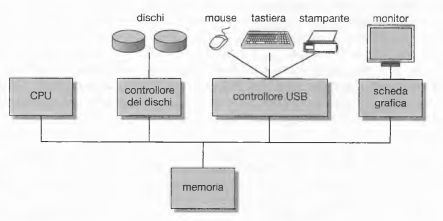
\includegraphics[scale=0.75]{img/0001.png}
\end{center}
La CPU e questi controllori possono operare in modo concor­rente, contendendosi i cicli d'accesso alla memoria. La sincronizzazione degli accessi alla
memoria è garantita dalla presenza di un controllore di memoria.
L'avviamento del sistema, conseguente all'accensione fisica di un calcolatore
richiede la presenza del \textbf{programma d'avviamento} (\textbf{bootstrap pro­gram}\index{bootstrap}), in genere contenuto in tipi di memoria noti con il termine generale di \textbf{firmware}\index{firmware}\footnote{Insieme delle istruzioni e delle applicazioni presenti permanentemente nella memoria di un sistema e che non possono essere modificate dall'utente.}, il
cui supporto fisico è parte integrante della macchina. Esempi di firmware sono le memorie
a sola lettura (read only memory, \textbf{ROM}), e le memorie programmabili cancellabili elettrica­mente (\textbf{EEPROM}). Il programma d'avviamento deve caricare nella memoria il siste­ma operativo e avviarne l'esecuzione, perciò individua e carica nella memoria il kernel del
sistema operativo; il sistema operativo avvia quindi l'esecuzione del primo processo d'elabo­razione, per esempio \texttt{init}, e attende che si verifichi qualche evento.

Un evento è di solito segnalato da un'interruzione dell'attuale sequenza d'esecuzione
della CPU, che può essere causata da un dispositivo fisico o da un programma. Nel primo
ca­so si parla di segnale d'interruzione o, più brevemente, \textbf{interruzione (interrupt)}.
Nel secondo caso si parla di segnale di eccezione
o, più brevemente, \textbf{eccezione (exception o trap)}, che può essere causata da un programma in
esecuzione a seguito di un evento eccezionale,
op­pure a seguito di una richiesta specifica effettuata da un programma utente per ottenere
l'e­secuzione di un servizio del sistema operativo, attraverso una speciale istruzione detta
\textbf{chia­mata di sistema (system call)\index{system call}} o \textbf{chiamata supervisore (supervisor call, SVC)}.
Ogniqualvolta riceve un segnale d'interruzione, la CPU interrompe l'elaborazione
cor­rente e trasferisce immediatamente l'esecuzione a una locazione fissa della memoria. Di
so­lito, questa locazione contiene l'indirizzo iniziale della procedura di servizio per quel dato
segnale d'interruzione. Una volta completata l'esecuzione della procedura richiesta, la CPU
riprende l'elaborazione precedentemente interrotta. Ciascun tipo di calcolatore ha il proprio meccanismo delle interruzioni.

Un segnale d'interruzione deve causare il trasferimento
del controllo all'appropriata procedura di servizio dell'evento a esso associato. Il modo più
semplice per gestire quest'operazione è quello di impiegare una procedura generale che
esa­mina le informazioni presenti nel segnale d'interruzione, e invoca la procedura di gestione
dello specifico segnale d'interruzione. la gestione di un'interruzione deve
esse­re molto rapida perciò si può usare una tabella di puntatori alle specifiche procedure.
In genere la tabella di puntatori
contenen­te gli indirizzi delle procedure di servizio delle interruzioni è mantenuta nella memoria
bas­sa (per esempio, le prime 100 locazioni). Questa sequenza d'indirizzi è detta
\textbf{vetto­re delle interruzioni}. Sistemi operativi radicalmente differenti, come Windows e
UNIX, usano lo stesso meccanismo di gestione delle interruzioni.

\subsubsection{Memorie}
La CPU può caricare istruzioni esclusivamente dalla memoria, quindi tutti i programmi da
eseguire devono esservi caricati. I computer general-purpose eseguono la maggior parte dei
programmi da una memoria riscrivibile, la  memoria
ad accesso diretto (\textbf{random access memory, RAM}). La memoria principale è realizzata solita­mente con una tecnologia basata su semiconduttori chiamata memoria dinamica ad
acces­so diretto (\textbf{dynamic random access memory, DRAM}). I computer utilizzano anche altri tipi di
memoria. Dal momento che la \textbf{memoria di sola lettura (ROM)} non può essere modificata,
vi sono salvati solo i programmi statici.

Tutte le tipologie di memoria forniscono un vettore di parole. Ciascuna parola
possie­de un proprio indirizzo. L'interazione avviene per mezzo di una sequenza di istruzioni \texttt{load}
e \texttt{store} opportunamente indirizzate. L'istruzione \texttt{load} trasferisce il contenuto di una pa­rola della memoria centrale in uno dei registri interni della CPU, mentre \texttt{store} copia il
con­tenuto di uno di questi registri nella locazione di memoria specificata.
La tipica sequenza d'esecuzione di un'istruzione, in un sistema con architettura di von
Neumann, comincia con il prelievo (\textbf{fetch}) di un'istruzione dalla memoria centrale e il suo
trasferimento nel registro d'istruzione. Quindi si decodifica (\textbf{decode}) l'istruzione
Una vol­ta terminata l'esecuzione (\textbf{execute}) dell'istruzione sugli operandi, il risultato si può scrivere nella memo­ria.

La maggior parte dei sistemi di calcolo comprende una \textbf{memoria secon­daria} come estensione della memoria centrale. La caratteristica fondamentale di questi di­spositivi è la capacità di conservare in modo permanente grandi quantità di informazioni.

Come già accennato, le memorie possono essere \textbf{volatili} e \textbf{non volatili}. La memoria volatile comporta la perdita dei dati nel caso di interruzione dell'alimentazione.

\subsubsection{I/O}
La memoria è solo uno dei numerosi dispositivi di I/O di un elaboratore. Un calcolatore d'uso generale è composto da una CPU e da un insieme di controllori di
dispositivi connessi mediante un bus comune. Ciascun controllore deve occuparsi di un
particolare tipo di dispositivo e, secondo la sua natura, può gestire uno o più dispositivi ad
es­so connessi.\\
Un controllore di dispositivo dispone di una propria me­moria interna, detta \textbf{memoria di transito (buffer)}\index{buffer}, e di un insieme di registri specializzati. Il
controllore è responsabile del trasferimento dei dati tra i dispositivi periferici a esso connes­si e la propria memoria di transito. I sistemi operativi in genere possiedono, per ogni controllore del dispositivo, un \textbf{driver del dispositivo} che si coordina con il controllore e funge
da interfaccia uniforme con il resto del sistema.

Per avviare un'operazione di I/O, il driver del dispositivo carica i registri interessati all'interno del controllore, il quale esamina i contenuti di questi registri per
scegliere l'azione da intraprendere. Il controllore comincia a trasferire i dati dal dispositivo al proprio buffer locale. A trasferimento
completato, il controllore informa il driver, tramite un'interruzione, di avere terminato l'o­perazione. Il driver passa quindi il controllo al sistema operativo, restituendo i dati se l'operazione è di lettura, altrimenti, restituisce le informazioni di stato.

In caso di trasferimenti massicci si utilizza
la tecnica dell'\textbf{accesso diretto alla memoria (DMA)}. Una volta impostati i buffer, i puntato­ri e i contatori necessari al dispositivo di I/O, il controllore trasferisce un intero blocco di da­ti dalla propria memoria buffer direttamente nella memoria centrale, o viceversa, senza al­cun intervento da parte della CPU.

Alcuni sistemi all'avanguardia hanno abbandonato la configurazione basata sul bus
per adottare un'architettura incentrata sugli switch, in cui più dispositivi fisici possono inte­ragire con varie parti del sistema concorrentemente, piuttosto che contendersi un unico bus
condiviso.

\subsection{Architettura degli elaboratori}
\subsubsection{Sistemi monoprocessore}
Un sistema monoprocessore è dotato di una CPU prin­cipale in grado di eseguire un insieme di istruzioni di natura generale. Quasi tutti i sistemi possiedono altri processori specializ­zati, deputati a compiti particolari. Tutti questi processori di tipo specifico sono dotati di un insieme ristretto di istruzio­ni, e non eseguono processi utenti.

\subsubsection{Sistemi multiprocessore}
Dispongono di più unità d'ela­borazione in stretta comunicazione, che condividono i canali di comunicazione all'interno
del calcolatore (bus), i timer dei cicli di macchina (clock) e talvolta i dispositivi di memoriz­zazione e periferici. Hanno tre vantaggi:
\begin{itemize}[noitemsep, leftmargin=*]
  \item Maggiore produttività (\textbf{throughput}\footnote{Quantità di dati trasmessi in una unità di tempo.}),
  \item Economia di scala,
  \item Incremento dell'affidabilità.
\end{itemize}
%
I sistemi multiprocessore attualmente in uso sono di due tipi. Alcuni impiegano la
\textbf{multielaborazione asimmetrica (asymmetric multiprocessing, AMP)}, in cui a ogni unità d'ela­borazione si assegna un compito specifico. Un'unità d'elaborazione principale controlla il si­stema, le altre attendono istruzioni dall'unità principale oppure hanno compiti predefiniti.\\
Nei sistemi più comuni si ricorre alla \textbf{multielaborazione simmetrica (symmetric multiprocessing, SMP)}, in cui ogni processore è abilitato al compimento di tutte le operazioni del
sistema. La tecnica SMP pone tutti i processori su un piano di parità; tra essi non vi è subor­dinazione gerarchica.

\subsubsection{Cluster di elaboratori}
I cluster di elaboratori \textbf{(clustered systems)} o cluster sono ba­sati sull'uso congiunto di più unità d'elaborazione riunite per lo svolgimento di attività d'ela­borazione comuni. Differiscono dai sistemi paralleli per il fatto che sono composti di due o
più calcolatori completi collegati tra loro.

\subsection{Struttura del sistema operativo}
Tra le più importanti caratteristiche dei sistemi operativi vi è la \textbf{multiprogrammazione}\index{multiprogrammazione}. In
generale, un singolo utente non è in grado di tenere costantemente occupati la CPU e i di­spositivi di I/O: la multiprogrammazione consente di aumentare la percentuale d'utilizzo
della CPU, organizzando i lavori in modo tale da mantenerla in continua attività.

Il sistema operativo tiene contem­poraneamente in memoria centrale diversi lavori. Dato che, in genere, la me­moria centrale è troppo piccola per contenere tutti i programmi da eseguire, questi vengono
collocati inizialmente sul disco in un'area apposita, detta \textbf{job pool}\index{job pool}, contenente tutti i pro­cessi in attesa di essere allocati nella memoria centrale.

Il sistema operativo ne sceglie uno tra quelli contenuti nella me­moria e inizia l'esecuzione: a un certo punto potrebbe trovarsi nell'attesa di qualche evento,
come il completamento di un'operazione di I/O. In questi casi, in un sistema non multiprogrammato, la CPU rimarrebbe inattiva. In un sistema con multiprogrammazione, invece, il
sistema operativo passa semplicemente a un altro lavoro e lo esegue. Quando il primo lavo­ro ha terminato l'attesa, la CPU ne riprende l'esecuzione. Finché c'è almeno un lavoro da
eseguire, la CPU non è mai inattiva.

La \textbf{partizione del tempo d'ela­borazione (time sharing o multitasking)}\index{multitasking} è un'estensione logica della multiprogrammazione.

\subsection{Attività del sistema operativo}
I moderni sistemi operativi sono guidati dalle interru­zioni. In assenza di processi da
eseguire e di utenti a cui rispondere, il sistema operativo rimane inerte e attende che accada
qualcosa.\\
A ciascun tipo di interruzione corrispondono nel sistema
singoli segmenti di codice, che determinano la reazione all'interruzione; apposite routine per
il servizio delle interruzioni hanno il compito di fornire loro una risposta adeguata.

\subsubsection{Duplice modalità di funzionamento}
Sono necessarie almeno due diverse modalità: \textbf{modalità utente} e \textbf{modalità di sistema}
(detta anche modalità kernel, modalità supervisore, modalità monitor o modalità privilegiata).
Per indicare quale sia la modalità attiva, l'architettura della CPU deve essere dotata di un bit,
chiamato appunto \textbf{bit di modalità}: di sistema (0) o utente (1).

All'avviamento del sistema, il bit è posto in modalità di sistema. Si carica il sistema
operativo che provvede all'esecuzione dei processi utenti in modalità utente. Ogni volta che
si verifica un'interruzione o un'eccezione si passa dalla modalità utente a quella di sistema,
prima di passare il controllo al programma uten­te, il sistema ripristina la modalità utente riportando a 1 il valore del bit.
La duplice modalità di funzionamento (dual mode) consente la protezione del sistema operativo rispetto al comportamento degli utenti e viceversa. Questo livello di protezione si ottiene definendo come istruzioni privilegiate le istruzioni di macchina che possono causare danni allo stato del sistema.

Le chiamate di sistema sono gli strumenti con cui un programma utente richiede al si­stema operativo di compiere operazioni a esso riservate. Una chiamata di sistema
è solitamente realizzata come un'eccezione che rimanda a un indirizzo specifico nel vettore
delle interruzioni. A tale eccezione si può dare esecuzione con un'istruzione \texttt{trap}\footnote{Eccezione. Ad es. accesso non consentito in memoria, divisione per 0, disconnessione dalla rete, errore di trasferimento dati a stampante.} generica,
sebbene alcuni sistemi abbiano un'i­struzione dedicata \texttt{syscall}.

\subsubsection{Timer}
Occorre im­pedire che un programma utente entri in un ciclo infinito o non richieda servizi del sistema
senza più restituire il controllo al sistema operativo. A tale scopo si può usare un \textbf{timer},
pro­grammabile affinché invii un segnale d'interruzione alla CPU a intervalli di tempo specificati, che possono essere fìssi (per esempio, di 1/60 di secondo) o variabili (per esempio, da un
millisecondo a un secondo). Un timer variabile di solito si realizza mediante un generatore
di impulsi a frequenza fissa e un contatore. Il sistema operativo assegna un valore al conta­tore, che si decrementa a ogni impulso e quando raggiunge il valore 0 si genera un segnale
d'interruzione.

Prima di restituire all'utente il controllo dell'esecuzione, il sistema assegna un valore al
timer. Se esso esaurisce, questo intervallo genera un'interruzione che causa il trasferimento
del controllo al sistema operativo, che può decidere se gestire le interruzioni come un erro­re fatale o concedere altro tempo al programma.

La presenza di un timer garantisce quindi che nessun programma utente possa essere
eseguito troppo a lungo.

\subsection{Gestione dei processi}
Un processo si può considerare come un programma in esecuzione.
Per svolgere i propri compiti, un processo necessita di alcune risorse, tra cui tempo di
CPU, memoria, file e dispositivi di I/O. Queste risorse si possono attribuire al processo al
momento della sua creazione, oppure si possono assegnare durante l'esecuzione.

Un programma di per sé non è un processo d'elaborazione; un programma è un'entità passiva
mentre un processo è un'entità attiva, con un \textbf{contatore di programma} che indica la successiva istruzione da eseguire.

L'esecuzione di un processo deve essere sequenziale: la
CPU esegue le istruzioni del processo una dopo l'altra, finché il processo termina; inoltre in
ogni istante si esegue al massimo un'istruzione del processo.

\subsection{Gestione della memoria}
La memoria centrale è fondamentale per il funzio­namento di un moderno sistema di calcolo. È un magazzino di dati velocemente accessibile ed è condivisa dalla CPU e da
alcuni dispositivi di I/O. La CPU legge le istruzioni dalla memoria centrale durante il ciclo di
prelievo delle istruzioni, oltre a leggere e scrivere i dati nella memoria centrale durante il ciclo
d'accesso ai dati (su di un'architettura Von Neumann). Anche il funzionamento dell'I/O rea­lizzato col DMA legge e scrive dati nella memoria centrale. Generalmente la memoria centra­le è l'unico ampio dispositivo di memorizzazione a cui la CPU può far riferimento e accedere
in modo diretto.

Per eseguire un programma è necessario che questo sia associato a indirizzi assoluti e
sia caricato nella memoria. Durante l'esecuzione del programma, la CPU accede alle proprie
istruzioni e ai dati provenienti dalla memoria. Quan­do il programma termina, si dichiara disponibile il suo spazio di memoria; a questo punto si può caricare ed eseguire il programma successivo.

\subsection{Sistemi distribuiti}
Per sistema distribuito\index{sistema distribuito} si intende un insieme di elaboratori collocati a distanza, e con carat­teristiche spesso eterogenee, interconnessi da una rete di calcolatori per consentire agli uten­ti l'accesso alle varie risorse dei singoli sistemi. L'accesso a una risorsa condivisa aumenta la
velocità di calcolo, la funzionalità, la disponibilità dei dati e il grado di affidabilità.

Una rete si può considerare, in parole semplici, come un canale di comunicazione tra
due o più sistemi. I sistemi distribuiti si basano sulle reti per realizzare le proprie funzioni.

Le reti differiscono per i protocolli
usati, per le distanze tra i nodi e per il mezzo attraverso il quale avviene la comunicazione.
Il più diffuso pro­tocollo di comunicazione è il TCP/IP.

Le reti si classificano secondo le distanze tra i loro nodi: una rete locale (LAN) com­prende nodi all'interno della stessa stanza, piano o edificio; una rete geografica (WAN) si
estende a gruppi di edifici, città, o al territorio di una regione o di uno stato.
Le reti metropolitane
(MAN) per esempio collegano gli edifici di un'intera città; i dispositivi BlueTooth e 802.11
comunicano a breve distanza, dell'ordine delle decine di metri, creando essenzialmente una
microrete (small-area network).

I mezzi di trasmissione che s'impiegano nelle reti sono altrettanto vari: fili di rame, fi­bre ottiche, trasmissioni via satellite, sistemi a microonde e sistemi radio.

\section{Strutture dei sistemi operativi}
Un sistema operativo offre un ambiente in cui eseguire i programmi e fornire servizi.
Ogni insieme di servizi offre funzionalità utili all'utente.
\begin{itemize}[leftmargin=*]
  \item Interfaccia con l'utente. Essa può assumere diverse forme: \textbf{a riga di comando (CLI)}, \textbf{a lotti} (pre­vede che comandi e relative direttive siano codificati nei file, eseguiti successivamente a lotti), \textbf{interfaccia grafica con l'utente (GUI)}.
  \item Esecuzione di un programma.
  \item Operazioni di I/O.
  \item Gestione del file system.
  \item Comunicazioni. Si possono realizzare tramite una \textbf{memoria condivisa} o attraverso lo \textbf{scambio di messaggi}.
  \item Rilevamento d'errori.
  \item Assegnazione delle risorse.
  \item Protezione e sicurezza.
\end{itemize}


\subsection{Chiamate di sistema}
Le chiamate di sistema\index{system call} costituiscono l'interfaccia tra un processo e il sistema operativo. Ta­li chiamate sono generalmente disponibili sotto forma di routine scritte in C o C++.

Anche programmi molto semplici possono fare un intenso uso del sistema operativo. Non è raro che un sistema ese­gua migliaia di chiamate di sistema al secondo.

La maggior parte dei programmatori, tuttavia, non si dovrà mai preoccupare di questi
dettagli: infatti, gli sviluppatori usano in genere un'interfaccia per la programmazione di
applicazioni \textbf{(API, application programming interface)}\index{API}. Essa specifica un insieme di funzioni a
disposizione dei programmatori, e dettagli ai parametri necessari all'invocazione di queste
funzioni, insieme ai valori restituiti. Tre delle interfacce più diffuse sono la API Win32 per i
sistemi Windows, la API POSIX per i sistemi basati sullo standard POSIX (UNIX, Linux e Mac OS X), e la API Java per la progettazione di applicazioni eseguite dalla macchina virtuale Java.

Le funzioni fornite da un API invocano solitamente le chiamate di si­stema per conto del programmatore. La funzione Win32 \texttt{CreateProcess()}, per esem­pio, che serve a generare un nuovo processo, invoca  \texttt{NTCreateProcess()}, una chiamata di sistema del kernel di Windows.

L'interfaccia in­tercetta le chiamate di sistema invocate dalla API, e richiede effettivamente la chiamata ne­cessaria.\medskip

Per passare parametri al sistema operativo si usano tre metodi generali: il più semplice consiste nel passare i parametri in registri; oppure si memorizzano i parametri in un blocco
o tabella di memoria e si passa l'indirizzo del blocco, in forma di parametro, in un registro; oppure il programma può anche col­locare (\emph{push}) i parametri in una pila da cui sono prelevati (\emph{pop}) dal sistema operativo.

\subsection{Categorie di chiamate di sistema}
Le chiamate di sistema sono classificabili approssimativamente in cinque categorie principa­li:
\begin{itemize}[noitemsep]
  \item \textbf{controllo dei processi}
  \item \textbf{gestione dei file}
  \item \textbf{gestione dei dispositivi}
  \item \textbf{gestione delle informa­zioni}
  \item \textbf{comunicazioni}.
\end{itemize}

\begin{center}
  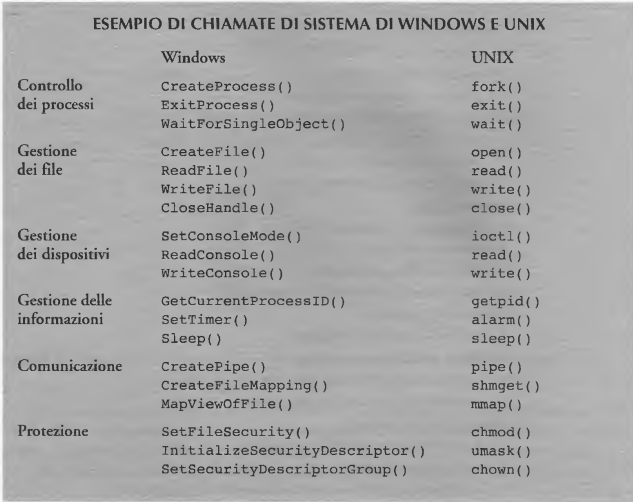
\includegraphics[scale=0.55]{img/0002.png}
\end{center}

\subsubsection{Controllo dei processi}
Un programma in esecuzione deve potersi fermare in modo sia normale (\texttt{end}) sia anormale (\texttt{abort}).

Talvolta si ha la registrazione in un file di un'im­magine del contenuto della memoria (\emph{dump}) e l'emissione di un messaggio d'errore. Uno specifico programma di ricerca e correzione degli errori (\emph{debugger}) può esaminare tali infor­mazioni per determinare le cause del problema.
Quando si presenta un errore, alcuni
sistemi permettono alle schede di controllo di indicare le specifiche azioni di recupero da in­
traprendere. La \textbf{scheda di controllo} è un comando per gestire l'esecuzione di un processo.

Un processo che esegue un programma può richiedere di caricare (\texttt{load}) ed eseguire
(\texttt{execute}) un altro programma.
Per creare n nuovo processo da sottoporre a multiprogrammazione, spessoo si fornisce una chiamata di siste­ma specifica, e precisamente \texttt{create process} oppure \texttt{submit job}).

Quando si crea un nuovo processo, è necessario mante­nerne il controllo. Ciò richiede la capacità di determinare e reimpostare gli attributi di un processo, compresi la sua priorità, il suo tempo massimo d'esecuzione e così via (\texttt{get process attributes} e \texttt{set process attributes}). Inoltre, può essere necessario terminare un
processo creato, se si riscontra che non è corretto o se non serve (\texttt{terminate process}).
Una volta creati, può essere necessario attendere che i processi terminino la loro esecu­zione. Quest'attesa si può impostare per un certo periodo di tempo (\texttt{wait} \emph{tempo}), ma è
più probabile che si preferisca attendere che si verifichi un dato evento (\texttt{wait} \emph{evento}). I processi devono quindi segnalare il verificarsi di quell'evento (\texttt{signal} \emph{evento}).

\subsubsection{Gestione dei file}
È necessario poter creare (\texttt{create}) e cancellare (\texttt{delete}) i file.
Una vol­ta creato il file è necessario aprirlo (\texttt{open}) e usarlo. Si può anche leggere (\texttt{read}), scrivere
(\texttt{write}) o riposizionare (\texttt{reposition}); si deve infine poter chiudere (\texttt{close}).
È inoltre necessario poter determinare i valori
degli attributi dei file (nome, tipo, codici di protezione) o delle directory ed eventualmente modificarli.
Per questa funzione sono richieste almeno due chiamate di sistema, e precisamente \texttt{get file attribute} e \texttt{set file attribute}. Alcuni sistemi operativi forniscono molte più
chiamate di sistema per spostare (\texttt{move}) e copiare (\texttt{copy}) file.

\subsubsection{Gestione dei dispositivi}
Per essere eseguito un programma necessita di parecchie risorse.
Le diverse risorse controllate dal sistema operativo si possono concepire come dei di­spositivi, alcuni dei quali sono in effetti dispositivi fisici (per esempio nastri), mentre altre
sono da considerarsi dispositivi astratti o virtuali (ad esempio file). In presenza di utenti
multipli, il sistema potrebbe prescrivere la richiesta (tramite \texttt{request}).
Dopo l'uso, avviene il rilascio (tramite \texttt{release}).
Una volta richiesto e assegnato il dispositivo, è possibile leggervi (\texttt{read}), scrivervi
(\texttt{write}) ed eventualmente procedere a un riposizionamento (\texttt{reposition}).

\subsubsection{Gestione delle informazioni}
Molte chiamate di sistema hanno semplicemente lo scopo di trasferire le informazioni tra il
programma utente e il sistema operativo. La maggior parte dei sistemi, per esempio, ha una
chiamata di sistema per ottenere l'ora (\texttt{time}) e la data attuali (\texttt{date}).
Un altro insieme di chiamate di sistema è utile per il debugging di programmi. Molti
sistemi operativi forniscono chiamate di sistema per ottenere un'immagine della memoria
(effettuare il \texttt{dump}\footnote{Il dump è un elemento di un database contenente un riepilogo della struttura delle tabelle del database medesimo e/o i relativi dati. Core dump: Varie porzioni fondamentali dello stato di programma sono di regola contestualmente annotate nel dump, compresi i registri del processore, il program counter e lo stack pointer, le informazioni di gestione della memoria ed altri flag ed informazioni attinenti al processore o al sistema operativo.})
Un programma di traccia­mento (\texttt{trace}) fornisce un elenco delle chiamate di sistema in esecuzione.\\
Il sistema operativo contiene inoltre informazioni su tutti i propri processi; a queste in­formazioni si può accedere tramite alcune chiamate di sistema. In genere esistono anche chia­mate di sistema per modificare le informazioni sui processi (\texttt{get process attributes} e \texttt{set process attributes}).

\subsubsection{Comunicazione}
Esistono due modelli molto diffusi di comunicazione tra processi: il modello a scambio di
messaggi e quello a memoria condivisa.

Nel modello \textbf{a scambio di messaggi}\index{modello a scambio di messaggi} i processi co­municanti si scambiano messaggi per il trasferimento delle informazioni sia direttamente sia
indirettamente attraverso una casella di posta comune. Prima di effettuare una comunica­
zione occorre aprire un collegamento. Il nome dell'altro comunicante deve essere noto;
tutti i calcolatori di una rete hanno
un \textbf{nome di macchina} (\emph{host name}), per esempio un nome IP, con il quale sono individuati.
Analogamente, ogni processo ha un \textbf{nome di processo}.
La conversione nell'iden­tificatore si compie con le chiamate di sistema \texttt{get hostid} e \texttt{get processid}. Questi identificatori sono quindi passati alle chiamate di sistema d'uso generale \texttt{open} e \texttt{close} oppure
alle chiamate di sistema specifiche \texttt{open connection} e \texttt{close connection}. Gene­ralmente il processo ricevente deve acconsentire alla comunicazione con una chiamata di si­stema \texttt{accept connection}. Nella maggior parte dei casi i processi che gestiscono la co­municazione sono \textbf{demoni} specifici.
Questi programmi eseguono una chiamata di sistema \texttt{wait for connection} e sono chiamati in causa quando si stabilisce un collegamento. L'origine della comu­nicazione, nota come \emph{client}, e il demone ricevente, noto come \emph{server}, possono quindi scam­biarsi i messaggi per mezzo delle chiamate di sistema \texttt{read message} e \texttt{write message}; la
chiamata di sistema \texttt{close connection} pone fine alla comunicazione.

Nel modello \textbf{a memoria condivisa},\index{modello a memoria condivisa} invece, i processi usano chiamate di sistema \texttt{chared memory create} e \texttt{shared memory attach} per creare e accedere alle aree di me­moria possedute da altri processi. Occorre ricordare che, normalmente, il sistema operativo
tenta di impedire a un processo l'accesso alla memoria di un altro processo.\\

Entrambi i metodi sono assai comuni e in certi sistemi operativi sono presenti con­temporaneamente. Lo scambio di messaggi è utile soprattutto quando è necessario trasferi­re una piccola quantità di dati;
la condivisione della memoria invece permette la massima ve­locità e convenienza nelle comunicazioni, ma sussistono proble­mi per quel che riguarda la protezione e la sincronizzazione tra processi che condividono la memoria.

\subsubsection{Protezione}
Tra le chiamate di sistema che offrono meccanismi di protezione vi sono solitamente la
\texttt{set permission} e la \texttt{let permission} che permettono di modificare i permessi di ac­
cesso a risorse come file e dischi. Le chiamate di sistema \texttt{allow user} e \texttt{deny user} speci­ficano se un particolare utente abbia il permesso di accesso a determinate risorse.

\subsubsection{Programmi di sistema}
I programmi di sistema offrono un ambiente più
conveniente per lo sviluppo e l'esecuzione dei programmi; alcuni sono semplici interfacce
per le chiamate di sistema, altri sono considerevolmente più complessi; in generale si posso­no classificare nelle seguenti categorie:
\begin{itemize}[leftmargin=*]
  \item \textbf{Gestione dei file}
  \item \textbf{Informazioni di stato}
  \item \textbf{Modifica dei file} - editor
  \item \textbf{Ambienti d'ausilio alla programmazione} - compilatori, assemblatori, programmi per
  la correzione degli errori, interpreti
  \item \textbf{Caricamento ed esecuzione dei programmi}
  \item \textbf{Comunicazioni}
\end{itemize}


\subsection{Struttura del sistema operativo}
\subsubsection{Struttura semplice}
Esistono si­stemi piccoli, semplici e limitati come l'MS-DOS in cui non vi è una netta separazione fra le interfacce e i livelli di funzionalità, tan­to che, per esempio, le applicazioni accedono direttamente alle routine di sistema per l'I/O, scrivendo direttamente sul video e sui dischi.\\ Libertà di questo genere rendono MS-DOS vul­nerabile agli errori e agli attacchi dei programmi utenti.
Il processore Intel 8088, per il quale fu scritto, non distingueva fra mo­dalità utente e di sistema, e non offriva protezione hardware.

Anche il sistema UNIX originale è poco strutturato: consiste di due parti separate, il ker­nel e i programmi di sistema. Il kernel è diviso in una serie di interfacce e driver
dei dispositivi, aggiunti ed espansi nel corso dell'evoluzione di UNIX.

\subsubsection{Metodo stratificato}
In presenza di hardware appropriato, i sistemi operativi possono essere suddivisi in moduli
più piccoli e gestibili di quanto non fosse possibile nelle prime versioni di MS-DOS e UNIX.\medskip\\
\begin{center}
  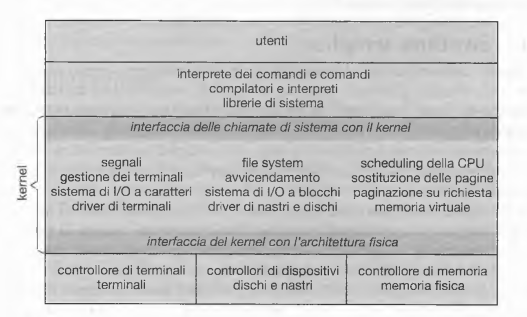
\includegraphics[scale=0.65]{img/0003.png}
\end{center}\medskip\\
Vi sono molti modi per rendere modulare un sistema operativo. Uno di loro è il \textbf{metodo stratificato}\index{metodo stratificato}, secondo il quale il sistema è suddiviso in un certo numero di livelli o stra­ti: il più basso corrisponde all'hardware (strato 0), il più alto all'interfaccia con l'utente
(strato N).\medskip\\
\begin{center}
  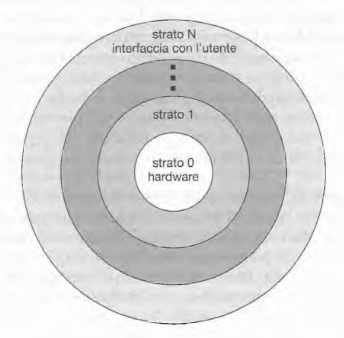
\includegraphics[scale=0.65]{img/0004.png}
\end{center}\medskip\\
Un tipico strato di sistema operativo (chiamato M) è
composto da strutture dati e da un insieme di routine richiamabili dagli strati di livello più alto.
Lo strato M, a sua volta, è in grado di invocare operazioni dagli strati di livello inferiore.

Attualmente si progettano sistemi basati su un numero inferiore di
strati con più funzioni, che offrono la maggior parte dei vantaggi del codice modulare, evi­tando i difficili problemi connessi alla definizione e all'interazione degli strati.

\subsubsection{Microkernel}
A mano a mano che il sistema operativo UNIX è stato esteso, il kernel è cresciuto notevol­mente, diventando sempre più diffìcile da gestire. Verso la metà degli anni '80 un gruppo di
ricercatori realizzò un sistema operativo, Mach,
col kernel strutturato in moduli secondo il cosiddetto orientamento a microkernel\index{microkernel}. Seguen­do questo orientamento si progetta il sistema operativo rimuovendo dal kernel tutti i com­ponenti non essenziali, realizzandoli come programmi di livello utente e di sistema. Ne ri­sulta un kernel di dimensioni assai inferiori.

Un microkernel offre i servizi minimi di gestione dei processi, della memoria e di
comunicazione.
Lo scopo principale del microkernel è fornire funzioni di comunicazione tra i pro­grammi client e i vari servizi, secondo il modello a scambio di messaggi.

Uno dei vantaggi del microkernel è la facilità di estensione del sistema operativo: i
nuovi servizi si aggiungono allo spazio utente e non comportano modifiche al kernel.
Offre maggiori garanzie di sicurezza e affidabilità, poiché i servizi si eseguono
in gran parte come processi utenti, e non come processi del kernel: se un servizio è compro­messo, il resto del sistema operativo rimane intatto.
I microkernel possono incorrere in cali di prestazioni dovuti al sovraccarico
indotto dall'esecuzione di processi utente con funzionalità di sistema.

\subsubsection{Moduli}
Il miglior approccio attualmente disponibile per la progettazione dei sistemi operativi
si fonda su tecniche della programmazione orientata agli oggetti per implementare un ker­nel modulare.
Il kernel è costituito da un insieme di componenti fondamentali, integrati poi da funzionalità aggiunte dinamicamente durante l'avvio o l'esecuzio­ne.

Questa organizzazione lascia la possibilità al kernel di fornire i servizi essenziali, ma permet­te anche di implementare dinamicamente certe caratteristiche. È possibile aggiungere driver
per dispositivi specifici, per esempio, o gestire file system diversi tramite moduli caricabili.

Cia­scun modulo può invocare funzionalità di un qualunque altro modulo.
Il modulo principale gestisce solo i servizi essenziali.

\subsection{Macchine virtuali}
L'idea alla base delle
macchine virtuali è di astrarre dalle unità hardware del singolo computer (CPU, memoria, ecc)
progettando per ciascuna unità un ambiente esecutivo soft­ware diverso, così da dare l'impressione che ognuno di loro giri sulla propria macchina.

Tramite lo scheduling\footnote{(Dall'inglese \emph{to schedule} - mettere in lista, pianificare) Lo schedulatore o gestore di processi è un programma che implementa un algoritmo di scheduling, ovvero stabilisce un ordinamento temporale per l'esecuzione di richieste di accesso ad una risorsa, tipicamente l'accesso al processore da parte di un processo da eseguire.} della CPU e la memoria virtuale il si­stema operativo può dare l'impressione che ogni processo sia dotato del proprio processore
e del proprio spazio di memoria (virtuale). La macchina virtuale fornisce un'interfaccia coin­cidente con il nudo hardware. Ogni processo ospite può usufruire di una copia (virtuale) del
calcolatore sottostante.

\subsubsection{Vantaggi}
Sono diverse le ragioni che portano alla creazione di una macchina virtuale, ma la maggior
parte è legata alla possibilità di condividere l'utilizzo concorrente dello stesso hardware in
diversi ambienti di esecuzione (ovvero diversi sistemi operativi).
Un vantaggio importante è che sistema ospitante è protetto dalle macchine virtuali, e
queste sono protette le une dalle altre. Un virus all'interno di un sistema operativo ospite
può danneggiare quel sistema operativo, ma è improbabile che colpisca il sistema ospitante
o altri sistemi ospiti.

Ogni macchina vir­tuale è completamente isolata dalle altre. Allo stesso tempo non vi è però una condivisione
diretta delle risorse. Per la condivisione delle risorse si seguono due approcci diversi. Il pri­mo prevede la possibilità di condividere un volume del file system, e quindi di condividere
file. Il secondo offre la possibilità di definire una rete di macchine virtuali, ognuna delle
quali sia in grado di inviare informazioni sulla rete privata virtuale. La rete è modellata co­me una rete fisica, ma è implementata via software.

Un altro vantaggio che le macchine virtuali offrono agli sviluppatori è dato dal fatto
che diversi sistemi operativi possono lavorare in concorrenza sulla stessa macchina. Una
workstation così configurata permette una rapida portabilità delle applicazioni su differenti
piattaforme e facilita la fase di test.

\subsubsection{Simulazione}
La virtualizzazione è soltanto uno dei numerosi metodi per emulare un si­stema. È il metodo più comune, perché fa in modo che il sistema operativo ospite e le appli­cazioni “credano” di essere in esecuzione su un hardware nativo. Visto che solo le risorse di
sistema devono essere virtualizzate, i processi ospitati possono girare quasi a piena velocità.

Un altro metodo di emulazione è la simulazione. In questo caso si ha un sistema ospi­tante con una propria architettura e un sistema ospite compilato per un'architettura diversa.
Supponiamo per esempio che un'azienda abbia sostituito i vecchi sistemi con sistemi più
nuovi, ma che voglia continuare a utilizzare alcuni importanti programmi compilati per i
vecchi sistemi. I programmi potrebbero essere mandati in esecuzione su un emulatore.
Il grosso limite sono le prestazioni.

\subsubsection{Paravirtualizzazione}
Un'altra variazione sul tema è la paravirtualizzazione. Piuttosto che provare a offrire al si­stema ospite una piattaforma identica a quella da esso desiderata, con la paravirtualizzazio­ne si cerca di rendere disponibile al sistema ospite un sistema simile, ma non identico, alle
sue preferenze.

\subsubsection{Macchina virtale Java}
Il linguaggio di programmazione Java fornisce una vasta libreria API e anche la definizione della macchi­na virtuale Java (Java Virtual machine, JVM).
Gli oggetti si specificano con il costrutto \texttt{class} e un programma consiste di una o più
classi. Per ognuna di queste, il compilatore produce un file (\texttt{.class}) contenente il cosid­detto \emph{bytecode}; si tratta di codice nel linguaggio di macchina della JVM, indipendente dal­l'architettura soggiacente, che viene per l'appunto eseguito dalla JVM.
La JVM è un calcolatore astratto che consiste di un caricatore delle classi e di un inter­prete del linguaggio che esegue il bytecode.

Il caricatore delle classi carica i fi­le \texttt{.class}, sia del programma scritto in Java sia dalla libreria API, affinché l'interprete pos­sa eseguirli. Dopo che una classe è stata caricata, il verificatore delle classi controlla la cor­rettezza a del codice bytecode. Se il controllo ha un esito positivo, la classe viene eseguita dall'interprete. La JVM gestisce la memoria in modo automatico procedendo alla sua “ripulitura”
(\emph{garbage collection}) che consiste nel recupero delle aree della memoria assegnate a oggetti
non più in uso per restituirla al sistema.

La JVM può essere implementata come software ospitato da un sistema operativo resi­dente, per esempio Windows, Linux o Mac OS X, oppure all'interno di un browser web. In
alternativa, può essere cablata in un circuito integrato espressamente progettato per l'esecu­zione di programmi Java. Nel primo caso, l'interprete Java interpreta le istruzioni bytecode
una alla volta. Una soluzione più efficiente consiste nell'uso di un compilatore istantaneo o
just-in-time (JIT). Alla prima invocazione di un metodo Java, il bytecode relativo è tradotto
in linguaggio macchina comprensibile dalla macchina fisica ospitante. Il codice macchina
relativo è poi salvato appropriatamente, in modo da essere direttamente riutilizzabile a una
successiva invocazione del metodo Java, evitando la lenta interpretazione delle istruzioni
bytecode. Il secondo caso fornisce una soluzione potenzialmente ancora più veloce, ovvero cablare la JVM in un circuito
integrato che esegua le istruzioni bytecode come codice macchina pri­mitivo, eliminando del tutto la necessità di interpreti e compilatori.

\subsection{Avvio del sistema}
La procedura d'avviamento di un calcolatore attraverso il caricamento del kernel
è nota come \textbf{avviamento} (\emph{booting}) del sistema: nella maggior parte dei sistemi di calcolo c'è
un piccolo segmento di codice, noto come \textbf{programma d'avvio} (\emph{bootstrap program})\index{bootstrap} o \textbf{carica­tore d'avvio} (\emph{bootstrap loader}), che individua il kernel, lo carica in memoria e ne avvia l'ese­cuzione. Alcuni sistemi, come i PC, eseguono tale compito in due fasi: un caricatore d'avvio
molto semplice preleva dal disco un più complesso programma d'avvio, che a sua volta cari­ca il kernel.

Quando una CPU sta per entrare in funzione - per esempio, quando l'elaboratore vie­ne acceso o riavviato - il registro delle istruzioni è caricato con una locazione di memoria
predefinita, da cui ha inizio l'esecuzione. Il programma di avvio inizia da questa locazione.
Esso è contenuto in una \textbf{memoria a sola lettura (read-only memory, ROM)}, poiché non si
conosce lo stato della RAM all'avvio del sistema; inoltre, la ROM presenta il vantaggio di non
dover essere inizializzata e di essere immune ai virus.

Il
programma di avvio può effettuare operazioni di vario genere. Una di queste, solita­mente, sottopone a diagnosi la macchina per ottenere informazioni sul suo stato. Se la dia­gnostica dà esito positivo, il programma è in grado di proseguire con le altre fasi di avvio.

Alcuni sistemi, come i telefoni cellulari, i PDA\footnote{Personal Digital Assistant: compter palmare.} e le console per videogiochi, memoriz­zano l'intero sistema operativo nella ROM. La scelta di custodire nella ROM il sistema opera­tivo si addice a sistemi di piccole dimensioni.
Questa soluzione comporta un problema, cioè la necessità di
modificare i circuiti ROM al fine di poter modificare il codice del programma di avvio. Alcu­ni sistemi ovviano a questo inconveniente utilizzando la \textbf{memoria a sola lettura program­mabile e cancellabile (EPROM)}, che è appunto a sola lettura, ma può diventare riscrivibile
qualora riceva un comando apposito. Tutte le forme di ROM sono anche dette firmware, in
considerazione delle loro caratteristiche, che sono un ibrido tra hardware e software.
Taluni sistemi memorizzano il sistema operativo nel firmware e lo
copiano nella RAM per eseguirlo rapidamente.

Per sistemi operativi di grandi dimensioni o per sistemi che cambiano di frequente, il caricatore di av­vio è memorizzato nel firmware e il sistema operativo risiede su disco.
Un disco che conten­ga una partizione di avvio è chiamato \textbf{disco di avvio} (\emph{boot disk}) o \textbf{disco di sistema}.

Una volta caricato il programma di avvio completo, esso può addentrarsi nel file sys­tem per localizzare il kernel, così da caricarlo in memoria e dare inizio alla sua esecuzione. E
solo a questo punto che il sistema può essere considerato in funzione (\textbf{running}).

\section{Processi}
I primi sistemi di calcolo consentivano l'esecuzione di un solo programma alla volta, che
aveva il completo controllo del sistema e accesso a tutte le sue risorse. Gli attuali sistemi consentono, invece, che più programmi siano caricati in memoria ed eseguiti in mo­do concorrente. Tale evoluzione richiede un più severo controllo e una maggiore comparti­mentazione dei vari programmi. Da tali necessità deriva la nozione di \textbf{processo d'elabora­zione} — o, più brevemente, \textbf{processo} - che in prima istanza si può definire come un pro­gramma in esecuzione.

Un sistema è quindi costituito da un insieme di processi: quelli del
sistema operativo eseguono il codice di sistema; gli utenti il codice utente. Tutti questi pro­cessi si possono eseguire potenzialmente in modo concorrente e l'uso della CPU è commutato tra i vari processi. Il sistema operativo può rendere il cal­colatore più produttivo avvicendando i diversi processi nell'uso della CPU.

\subsection{Concetto di processo}
Un \textbf{sistema a lotti} (\emph{batch}) esegue lavori (\emph{job}), mentre un sistema a partizione del tem­po esegue \textbf{programmi utenti} o \textbf{task}. Anche se l'utente esegue un solo programma alla volta, il sistema operativo deve svolge­re le proprie attività interne, per esempio la gestione della memoria. Queste attività sono si­mili per molti aspetti, perciò sono denominate processi.
In questo testo i termini lavoro e processo sono usati in modo quasi intercambiabile.

\subsubsection{Processo}
Un processo è un programma in esecuzione. Comprende l'attività corrente,
rappresentata dal valore del contatore di programma e dal contenuto dei registri della CPU;
normalmente comprende anche la propria \textbf{pila} (\emph{stack}), contenente a sua volta i dati tempo­ranei, come i parametri di un metodo, gli indirizzi di rientro e le variabili locali, e una sezio­ne di dati contenente le variabili globali. Un processo può includere uno \textbf{heap}, ossia della
memoria dinamicamente allocata durante l'esecuzione del processo.

Un programma è un'enti­tà \emph{passiva}, come il contenuto di un file memorizzato in un disco, mentre un processo è un'en­tità \emph{attiva}, con un contatore di programma che specifica qual è l'istruzione successiva da ese­guire e un insieme di risorse associate. Un programma diventa un processo quando il file
eseguibile che lo contiene è caricato in memoria.

Sebbene due processi siano associabili allo stesso programma, sono tuttavia da consi­derare due sequenze d'esecuzione distinte.

\subsubsection{Stato del processo}
Un processo durante l'esecuzione è soggetto a cambiamenti di stato.
Ogni processo può trovarsi in uno tra i seguenti stati:\medskip\\
- Nuovo;\medskip\\
- Esecuzione;\medskip\\
- Attesa;\medskip\\
- Pronto;\medskip\\
- Terminato.\medskip\\
Queste definizioni sono piuttosto arbitrarie, e variano secondo il sistema operativo.
In ciascuna unità d'ela­borazione può essere in esecuzione solo un processo per volta, sebbene molti processi possa­no essere pronti o nello stato di attesa.\medskip\\
\begin{center}
  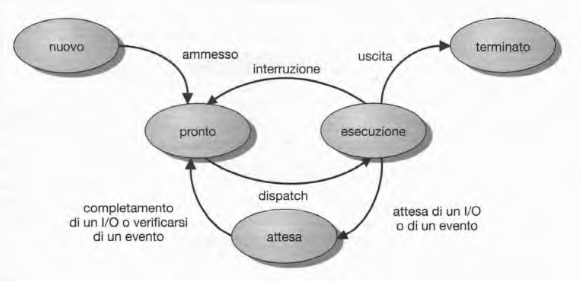
\includegraphics[scale=0.6]{img/0005.png}\\
  \caption{Diagramma di transizione degli stati di un processo.}
\end{center}

\subsubsection{Blocco di controllo dei processi}
Ogni processo è rappresentato nel sistema operativo da un \textbf{blocco di controllo di un pro­cesso} (\emph{process control block},\index{process control block} PCB, o \emph{task control block}, TCB). Esso contiene molte informazioni connesse a un processo specifico, come:
\begin{itemize}[leftmargin=*, noitemsep]
  \item \textbf{Stato del processo};
  \item \textbf{Contatore di programma}: contiene l'indirizzo della suc­cessiva istruzione da eseguire per tale processo;
  \item \textbf{Registri di CPU}: I registri variano in numero e tipo secondo l'architettura del calcola­
  tore. Essi comprendono accumulatori, registri d'indice, puntatori alla cima delle strut­ture a pila (\emph{stackpointer}), registri d'uso generale e registri contenenti informazioni re­lative ai codici di condizione. Quando si verifica un'interruzione della CPU, si devono
  salvare tutte queste informazioni insieme con il contatore di programma;
  \item \textbf{Informazioni sullo scheduling di CPU};
  \item \textbf{Informazioni sulla gestione della memoria};
  \item \textbf{Informazioni di contabilizzazione delle risorse};
  \item \textbf{Informazioni sullo stato dell'I/O}.
\end{itemize}


\begin{center}
  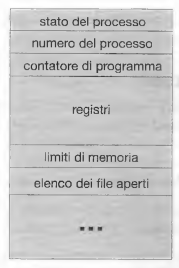
\includegraphics[scale=0.7]{img/0006.png}
\end{center}

\subsubsection{Thread}
Un processo è un programma che si esegue seguendo un unico percorso d'esecuzione, detto \textbf{thread}.

\subsection{Scheduling dei processi}
L'obiettivo della multiprogrammazione consiste nel disporre dell'esecuzione contemporanea
di alcuni processi in modo da massimizzare l'utilizzo della CPU. Lo scheduler dei processi seleziona un processo da eseguire dall'insieme di
quelli disponibili. Nei sistemi monoprocessore non vi sarà mai più di un processo in esecu­zione: gli altri dovranno attendere finché la CPU sia nuovamente disponibile.

\subsubsection{Code di scheduling}
Ogni processo è inserito in una \textbf{coda di processi}, composta da tutti i processi del sistema. I
processi presenti in memoria centrale, che sono pronti e nell'attesa d'essere eseguiti, si tro­vano in una lista detta \textbf{coda dei processi pronti} (\emph{ready queue}). Questa coda generalmente si
memorizza come una lista concatenata.
L'elenco dei processi che attendono la disponibilità di un particolare dispositivo di I/O si chiama
\textbf{coda del dispositivo}; ogni dispositivo ha la propria coda.

Un nuovo processo si colloca inizialmente nella coda dei processi pronti, dove attende
finchè non è selezionato per essere eseguito (\emph{dispatched}). Al termine della sua esecuzione viene allontanato da tutte le code, rimosso il suo PCB e revocate le varie ri­sorse.
\begin{center}
  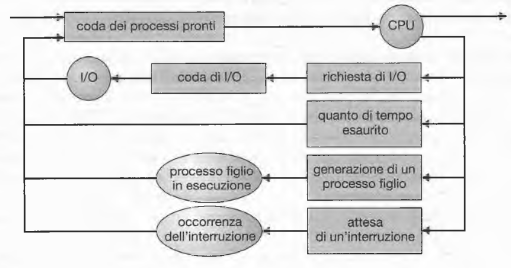
\includegraphics[scale=0.7]{img/0007.png}
\end{center}

\subsubsection{Scheduler}
Nel corso della sua esistenza, un processo si trova in varie code di scheduling. Il sistema ope­rativo, incaricato di selezionare i processi dalle suddette code, compie la selezione per mez­zo di un opportuno \textbf{scheduler}\index{scheduler}.

In un sistema a lotti, accade che si sottopongano più processi di quanti se ne
possano eseguire immediatamente. Questi lavori si trasferiscono in dispositivi di memoria
secondaria, dove si tengono fino al momento dell'esecuzione (\emph{spooling}). Lo \textbf{scheduler a lungo termine} (\emph{job scheduler}), sceglie i lavori da questo insieme e li ca­rica in memoria affinché siano eseguiti. Lo \textbf{scheduler a breve termine}, o \textbf{scheduler di CPU},
fa la selezione tra i lavori pronti per l'esecuzione e assegna la CPU a uno di loro.
Lo scheduler a breve termine seleziona frequentemente; deve essere molto rapido.
Lo scheduler a lungo termine si esegue con una frequenza molto inferiore;
e controlla il grado di multiprogrammazione, cioè il numero di
processi presenti in memoria.

In generale, la maggior parte dei processi si può caratterizzare come avente una prevalen­za di I/O, o come avente una prevalenza d'elaborazione. Un processo con prevalenza di I/O
(\emph{I/O bound}) impiega la maggior parte del proprio tempo nell'esecuzione di operazioni di I/O.
Un processo con prevalenza d'elaborazione (\emph{CPU bound}), al contrario, richiede poche opera­zioni di I/O e impiega la maggior parte del proprio tempo nelle elaborazioni. E fondamen­tale che lo scheduler a lungo termine selezioni una buona combinazione di processi con
prevalenza di I/O e con prevalenza d'elaborazione.

In alcuni sistemi operativi come quelli a partizione del tempo, si può introdurre un li­vello di scheduling intermedio. Questo è detto \textbf{scheduler a medio termine}.
L'idea alla base di un tale scheduler è che a volte può essere van­taggioso eliminare processi dalla memoria (e dalla contesa attiva per la CPU), riducendo il
grado di multiprogrammazione del sistema. In seguito, il processo può essere reintrodotto
in memoria, in modo che la sua esecuzione riprenda da dove era stata interrotta.
Questo schema si chiama \textbf{avvicendamento dei processi in memoria} — o, più in breve,
\textbf{avvicendamento} (\emph{swapping})\index{swapping}.

\subsubsection{Cambio di contesto}
Sono le interruzioni a indurre il sistema a sospendere il
lavoro attuale della CPU per eseguire routine del kernel. In presenza di una interruzione, il sistema deve salvare il
contesto del processo corrente, per poterlo poi ripristinare quando il processo stesso potrà
ritornare in esecuzione. Il contesto è rappresentato all'interno del PCB del processo, e com­
prende i valori dei registri della CPU, lo stato del processo, e informa­zioni relative alla gestione della memoria. In termini generali, si esegue un \textbf{salvataggio dello
stato corrente della CPU}, si attuerà un corrispondente \textbf{ripristino dello stato} per poter riprendere l'elaborazio­ne.\medskip\\
Il passaggio della CPU a un nuovo processo implica la registrazione dello stato del pro­cesso vecchio e il caricamento dello stato precedentemente registrato del nuovo processo.
Questa procedura è nota col nome di \textbf{cambio di contesto} (\emph{contest switch}).

\subsection{Operazioni sui processi}
\subsubsection{Creazione di un processo}
Durante la propria esecuzione, un processo può creare numerosi nuovi processi tramite
un'apposita chiamata di sistema (\texttt{create\_process}). Il processo creante si chiama proces­so \textbf{genitore}, mentre il nuovo processo si chiama processo \textbf{figlio}. Ciascuno di questi nuovi
processi può creare a sua volta altri processi, formando un albero di processi.

La maggior parte dei sistemi operativi identi­fica un processo per mezzo di un numero univoco, detto \textbf{identificatore del processo} o \textbf{pid}\index{pid} (\emph{process identifier}).
Nei sistemi UNIX si può ottenere l'elenco dei processi tramite il comando \texttt{ps}. Digitan­do \texttt{ps -el} si otterranno informazioni complete su tutti i processi attualmente attivi nel si­stema.
\medskip\\
Quando un processo ne crea uno nuovo, per quel che riguarda l'esecuzione ci sono
due possibilità:
\begin{enumerate}
  \item il processo genitore continua l'esecuzione in modo concorrente con i propri processi
  figli;
  \item il processo genitore attende che alcuni o tutti i suoi processi figli terminino.
\end{enumerate}
Ci sono due possibilità anche per quel che riguarda lo spazio d'indirizzi del nuovo processo:
\begin{enumerate}
  \item il processo figlio è un duplicato del processo genitore;
  \item nel processo figlio si carica un nuovo programma.
\end{enumerate}
%
Nel sistema operativo UNIX, un processo si crea per mezzo della chiamata di
sistema \texttt{fork()},\index{fork()} ed è composto di una copia dello spazio degli indirizzi del processo geni­tore. Questo meccanismo permette al processo genitore di comunicare senza difficoltà con
il proprio processo figlio. Entrambi i processi (genitore e figlio) continuano l'esecuzione al­
l'istruzione successiva alla chiamata di sistema \texttt{fork()}, con una differenza: la chiamata di
sistema \texttt{fork()} riporta il valore zero nel nuovo processo (il figlio), ma riporta l'identifica­tore del processo figlio (il PID diverso da zero) nel processo genitore. Tramite il valore ripor­tato del PID, i due processi possono procedere nell'esecuzione “sapendo” qual è il processo
padre e qual è il processo figlio.

Generalmente, dopo una chiamata di sistema \texttt{fork()}, uno dei due processi impiega
una chiamata di sistema \texttt{exec()} per sostituire lo spazio di memoria del processo con un
nuovo programma.

Il processo genitore può anche generare più processi
figli, oppure, se durante l'esecuzione del processo figlio non ha nient'altro da fare, può in­
vocare la chiamata di sistema \texttt{wait()} per rimuovere se stesso dalla coda dei processi pronti
fino alla terminazione del figlio.

\subsubsection{Terminazione di un processo}
Un processo termina quando finisce l'esecuzione della sua ultima istruzione e inoltra la ri­chiesta al sistema operativo di essere cancellato usando la chiamata di sistema \texttt{exit()}\index{exit()};
il processo figlio può riportare alcuni dati al processo genitore, che li riceve
attraverso la chiamata di sistema \texttt{wait()}. Tutte le risorse del processo,
sono liberate dal sistema ope­rativo.

La terminazione di un processo si può verificare anche in altri casi. Un processo può
causare la terminazione di un altro per mezzo di un'opportuna chiamata di sistema (per
esempio \texttt{TerminateProcess()} in Win32). Generalmente solo il genitore del processo
che si vuole terminare può invocare una chiamata di sistema di questo tipo.

Occorre notare che un genitore deve conoscere le identità dei propri figli, perciò quando un
processo ne crea uno nuovo, l'identità del nuovo processo viene passata al processo genitore.
Un processo genitore può porre termine all'esecuzione di uno dei suoi processi figli
per diversi motivi:
\begin{itemize}[noitemsep, leftmargin=*]
  \item Il processo figlio ha ecceduto nell'uso di alcune tra le risorse che gli sono state assegna­te.
  \item Il compito assegnato al processo figlio non è più richiesto.
  \item Il processo genitore termina e il sistema operativo non consente a un processo figlio di
  continuare l'esecuzione in tale circostanza.
\end{itemize}
In alcuni sistemi, fra i quali VMS, se un processo termina si devono terminare anche i suoi fi­gli, indipendentemente dal fatto che la terminazione del genitore sia stata normale o anormale. Si parla di \textbf{terminazione a cascata}.

\subsection{Comunicazione tra processi}
I processi eseguiti concorrentemente nel sistema operativo possono essere indipendenti o cooperanti. Un processo è indipendente se non può influire su altri processi del sistema o subirne l'influsso. Un processo che non condivide dati con altri processi è indipendente; Un processo è cooperante se influenza o può essere influenzato da altri processi in esecuzione nel sistema.

Qualsia­si processo che condivide dati con altri processi è un processo cooperante.
Un ambiente che consente la cooperazione tra processi può essere utile per diverse ragioni:
\begin{itemize}[leftmargin=*]
  \item \textbf{Condivisione d'informazioni};
  \item \textbf{Accelerazione del calcolo}: alcune attività d'elaborazione sono realizzabili più rapida­mente se si suddividono in sottoattività eseguibili in parallelo;
  \item \textbf{Modularità};
  \item \textbf{Convenienza}.
\end{itemize}
%
Per lo scambio di dati e informazioni i processi cooperanti necessitano di un meccanismo di
comunicazione tra processi (IPC, \emph{interprocess communication})\index{IPC}. I modelli fondamentali della
comunicazione tra processi sono due: (1) a memoria condivisa e (2) a scambio di messag­gi.

Nei sistemi operativi sono diffusi entrambi i modelli; a volte coesistono in un unico si­stema. Lo scambio di messaggi è utile per trasmettere piccole quantità di dati. La memoria condivisa massimizza l'efficienza della comunicazio­ne, ed è più veloce dello scambio di messaggi, che è solitamente implementato tramite chia­mate di sistema che impegnano il kernel; la memoria condivisa, invece, richiede l'intervento
del kernel solo per allocare le regioni di memoria condivisa, dopo di che tutti gli accessi sono
gestiti alla stregua di ordinari accessi in memoria che non richiedono l'assistenza del kernel.

\subsubsection{Sistemi a memoria condivisa}
La comunicazione tra processi basata sulla condivisione della memoria\index{modello a memoria condivisa} richiede che i pro­cessi comunicanti allochino una zona di memoria condivisa, di solito residente nello spazio
degli indirizzi del processo che la alloca.

Si ricordi che, normalmente, il siste­ma operativo tenta di impedire a un processo l'accesso alla memoria di altri processi. La condivisione della memoria richiede che due o più processi raggiungano un accordo per su­perare questo limite.

Si consideri il problema del pro­duttore/consumatore; tale problema è un usuale paradigma per processi cooperanti. Un
processo \textbf{produttore} produce informazioni che sono consumate da un processo \textbf{consumato­re}.
L'esecuzione concorrente dei due processi richiede la presenza di un buffer che
possa essere riempito dal produttore e svuotato dal consumatore.
Sono utilizzabili due tipi di buffer. Quello \textbf{illimitato} non pone limiti alla dimensione del
buffer. Il consumatore può trovarsi ad attendere nuovi oggetti, ma il produttore può sempre
produrne. Il problema del produttore e del consumatore con \textbf{buffer limitato} presuppone l'esi­stenza di una dimensione fissa del buffer in questione. In questo caso, il consumatore deve at­tendere che il buffer sia vuoto; viceversa, il produttore deve attendere che il buffer sia pieno.

\subsubsection{Sistemi a scambio di messaggi}
Lo scambio di messaggi\index{modello a scambio di messaggi} è un meccanismo che permette a due o più processi di comu­nicare e di sincronizzarsi senza condividere lo stesso spazio degli indirizzi. È una tecnica par­ticolarmente utile negli ambienti distribuiti.

Un meccanismo per lo scambio di messaggi deve prevedere almeno due operazioni: \texttt{send} (cioè, “invia messaggio”) e \texttt{receive} (cioè, “ricevi messaggio”). I messaggi possono
avere lunghezza fissa o variabile. Nel primo caso, l'implementazione a livello del sistema è
elementare, ma programmare applicazioni diviene più complicato. Nel secondo caso, l'implementazione del meccanismo è più complessa, mentre la programmazione utente risulta
semplificata.
Se i processi P e Q vogliono comunicare, devono inviare e ricevere messaggi tra loro;
dunque deve esistere un canale di comunicazione (\emph{communication link}).\index{communication link}
\medskip\\
Ci sono diversi metodi per realizzare a livello logico un canale di comunicazione e le ope­razioni \texttt{send()} e \texttt{receive()}:
\begin{itemize}[noitemsep, leftmargin=*]
  \item comunicazione diretta o indiretta;
  \item comunicazione sincrona o asincrona;
  \item gestione automatica o esplicita del buffer.
\end{itemize}
%
\textbf{Comunicazione diretta}\\
Con la comunicazione diretta, ogni processo che intenda comunicare deve nominare
esplicitamente il ricevente o il trasmittente della comunicazione. In questo schema le fun­zioni primitive \texttt{send()} e \texttt{receive()} si definiscono come segue:\medskip\\
- send(P, messaggio), invia messaggio al processo P;\medskip\\
- receive(Q, messaggio), riceve, in messaggio, un messaggio dal processo Q.\medskip\\
All'interno di questo schema, un canale di comunicazione ha le seguenti caratteristiche:\medskip\\
- tra ogni coppia di processi che intendono comunicare si stabilisce automaticamente
un canale; i processi devono conoscere solo la reciproca identità;\medskip\\
- un canale è associato esattamente a due processi.\medskip\\
Questo schema ha una \emph{simmetria} nell'indirizzamento, vale a dire che per poter comu­nicare, il trasmittente e il ricevente devono nominarsi a vicenda. Una variante di questo
schema si avvale dell'\emph{asimmetria} dell'indirizzamento: soltanto il trasmittente nomina il rice­vente, mentre il ricevente non deve nominare il trasmittente. In questo schema le primitive
\texttt{send()} e \texttt{receive()} si definiscono come segue:\medskip\\
- send(P, messaggio), invia messaggio al processo P;\medskip\\
- receive(id, messaggio), riceve, in messaggio, un messaggio da qualsiasi processo; nella
variabile id si riporta il nome del processo con cui è avvenuta la comunicazione.\medskip\\
%
\textbf{Comunicazione indiretta}\\
Con la comunicazione indiretta, i messaggi s'inviano a delle porte (dette anche \emph{mailbox})\index{mailbox}, che li ricevono. Una porta si può considerare in modo astratto come un oggetto in cui
i processi possono introdurre e prelevare messaggi, ed è identificata in modo unico.
In questo schema un processo può comunicare con altri processi tramite un certo numero di
porte. Due processi possono comunicare solo se condividono una porta. Le primitive
\texttt{send()} e \texttt{receive()} si definiscono come segue:\medskip\\
- send(A, messaggio), invia messaggio alla porta A;\medskip\\
- receive(A, messaggio), riceve, in messaggio, un messaggio dalla porta A.\medskip\\
Il canale di comunicazione ha le seguenti caratteristiche:\medskip\\
- tra una coppia di processi si stabilisce un canale solo se entrambi i processi della cop­pia condividono una stessa porta;\medskip\\
- un canale può essere associato a più di due processi;\medskip\\
- tra ogni coppia di processi comunicanti possono esserci più canali diversi, ciascuno
corrispondente a una porta.\medskip\\
Si supponga che i processi $P_1, P_2,$ e $P_3$ condividano la porta $A$. II processo $P_1$
invia un messaggio ad $A$, mentre sia $P_2$ sia $P_3$ eseguono una \texttt{receive()} da $A$.\\
Sorge il pro­blema di sapere quale processo riceverà il messaggio. La soluzione dipende dallo schema pre­scelto:\medskip\\
- si può fare in modo che un canale sia associato al massimo a due processi;\medskip\\
- si può consentire l'esecuzione di un'operazione \texttt{receive()} a un solo processo alla volta;\medskip\\
- si può consentire al sistema di decidere arbitrariamente quale processo riceverà il mes­saggio.\medskip\\
Il sistema può
anche definire un algoritmo per selezionare quale processo riceverà il messaggio
e può comunicare l'identità del ricevente al trasmittente.\medskip\\
%
Una porta può appartenere al processo o al sistema. Se appartiene a un processo, cioè fa par­te del suo spazio d'indirizzi, occorre distinguere ulteriormente tra il proprietario, che può
soltanto ricevere messaggi tramite la porta, e l'utente, che può solo inviare messaggi alla por­ta. Ogni porta ha un unico proprietario.\\
Una porta posseduta dal sistema operativo è indipendente e non è legata
ad alcun processo particolare. Il sistema operativo offre un meccanismo che permette a un
processo le seguenti operazioni:\medskip\\
- creare una nuova porta;\medskip\\
- inviare e ricevere messaggi tramite la porta;\medskip\\
- rimuovere una porta.\medskip\\
Il processo che crea una nuova porta è il proprietario predefinito della porta, inizialmente è
l'unico processo che può ricevere messaggi attraverso questa porta. Tuttavia, il diritto di pro­prietà e il diritto di ricezione si possono passare ad altri processi per mezzo di idonee chia­mate di sistema.\medskip\\
%
\textbf{Sincronizzazione}\\
La comunicazione tra processi avviene attraverso chiamate delle primitive \texttt{send()} e \texttt{receive()}. Ci sono diverse possibilità nella definizione di ciascuna primitiva. Lo scambio
di messaggi può essere \textbf{sincrono (o bloccante)}\index{comunicazione sincrona} oppure \textbf{asincrono (o non bloccante)}\index{comunicazione asincrona}.
- Invio sincrono. Il processo che invia il messaggio si blocca nell'attesa che il processo ri­cevente, o la porta, riceva il messaggio.
\begin{itemize}[noitemsep, leftmargin=*]
  \item Invio asincrono. Il processo invia il messaggio e riprende la propria esecuzione.
  \item Ricezione sincrona. Il ricevente si blocca nell'attesa dell'arrivo di un messaggio.
  \item Ricezione asincrona. Il ricevente riceve un messaggio valido oppure un valore nullo.
\end{itemize}
%
Se le primitive \texttt{send()} e \texttt{receive()} sono entrambe bloccanti si parla di \textbf{rendez-vous}\index{rendez-vous} tra mittente e ricevente.\medskip\\
%
\textbf{Code di messaggi}\\
I messaggi scambiati tra processi comunicanti risie­dono in code temporanee.
Esistono tre modi per realizzare queste code:
\begin{itemize}[leftmargin=*]
  \item \textbf{Capacità zero}. La coda ha lunghezza massima 0, quindi il canale non può avere mes­saggi in attesa al suo interno. In questo caso il trasmittente deve fermarsi finché il rice­vente prende in consegna il messaggio. (Solo rendezvous).
  \item \textbf{Capacità limitata}. La coda ha lunghezza finita $n$, quindi al suo interno possono risie­dere al massimo $n$ messaggi.
  \item \textbf{Capacità illimitata}. La coda ha una lunghezza potenzialmente infinita, quindi al suo in­terno può attendere un numero indefinito di messaggi. Il trasmittente non si ferma mai.
\end{itemize}
%
Il caso con capacità zero è talvolta chiamato sistema a scambio di messaggi senza memoriz­zazione transitoria (\emph{no buffering})\index{buffering}; gli altri due, sistemi con memorizzazione transitoria auto­matica (\emph{automatic buffering}).

\subsection{Comunicazione nei sistemi client-server}
Ci siamo soffermati su come i processi possano comunicare usando me­moria condivisa e scambio di messaggi. Tali tecniche sono utilizzabili anche per la comuni­cazione tra sistemi client/server. Consideriamo qui altre tre strategie: soc­ket, chiamate di procedura remote (RPC)\index{RPC} e invocazione di metodi remoti (RMI)\index{RMI}.

\subsubsection{Socket}
Una \textbf{socket}\index{socket} è definita come l'estremità di un canale di comunicazione. Una coppia di proces­si che comunica attraverso una rete usa una coppia di socket, una per ogni processo, e ogni
socket è identificata da un indirizzo IP concatenato a un numero di porta. Le
socket impiegano un'architettura client-server; il server attende le richieste dei client, stando
in ascolto a una porta specificata; quando il server riceve una richiesta, se accetta la connes­sione proveniente dalla socket del client, si stabilisce la comunicazione. I server che svolgo­no servizi specifici (come telnet, ftp, e http) stanno in ascolto a porte note (i server telnet al­
la porta 23, i server ftp alla porta 21, e i server Web o http alla porta 80). Tutte le porte al di
sotto del valore 1024 sono considerate note e si usano per realizzare servizi standard.

Quando un processo client richiede una connessione, il calcolatore che lo esegue asse­gna una porta specifica, che consiste di un numero arbitrario maggiore di 1024.
Si supponga
per esempio che un processo client presente nel calcolatore X con indirizzo IP 146.86.5.20
voglia stabilire una connessione con un server Web (in ascolto alla porta 80) all'indirizzo
161.25.19.8; il calcolatore X potrebbe assegnare al client, per esempio, la porta 1625. La con­
nessione sarebbe composta di una coppia di socket: (146.86.5.20:1625) nel calcolatore X e
(161.25.19.8:80) nel server Web.

Tutte le connessioni devono essere uniche; quindi, se un altro processo, nel calcolato­re X, vuole stabilire un'altra connessione con lo stesso server Web, riceve un numero di por­ta maggiore di 1024 e diverso da 1625.
\medskip\\
Il linguaggio Java prevede tre tipi differenti di socket: quelle \textbf{orientate alla connessio­ne} (TCP)\index{TCP} sono realizzate con la classe Socket; quelle \textbf{prive di connessione} (UDP)\index{UDP} usano la
classe DatagramSocket; il terzo tipo di socket è basato sulla classe \texttt{MulticastSocket}; si
tratta di una sottoclasse della classe \texttt{DatagramSocket} che permette l'invio simultaneo dei
dati a diversi destinatari (\emph{multicast}).
Il \textbf{loopback}\index{loopback} è un indirizzo usato da una macchina per riferirsi a se stessa. Tramite questo stratagemma, un client e un server residenti sulla stessa macchina sono
in grado di comunicare tramite il protocollo TCP/IP.\index{TCP/IP}

Le socket permettono unica­mente la trasmissione di un flusso non strutturato di byte: è responsabilità del client e del
server interpretare e organizzare i dati in forme più complesse.

\subsubsection{Chiamate di procedure note}
La RPC\index{RPC} è stata progettata per astrarre il meccanismo della chiamata di pro­cedura affinché si possa usare tra sistemi collegati tramite una rete. Per molti aspetti è simile al
meccanismo IPC\index{IPC} ma, contrariamente a quel che accade nella funzione IPC, i messaggi scambiati per la co­municazione RPC sono ben strutturati e non semplici pacchetti di dati.

Si indirizzano a un de­mone di RPC, in ascolto a una porta del sistema remoto, e contengono un identificatore della funzione da eseguire e i parametri da inviare a tale funzione. Nel sistema remoto si esegue que­sta funzione e si invia ogni risultato al richiedente in un messaggio distinto.
La porta è semplicemente un numero inserito all'inizio dei pacchetti di messaggi.

La semantica delle RPC permette a un client di richiamare una procedura presente in
un sistema remoto nello stesso modo in cui invocherebbe una procedura locale. Il sistema
delle RPC nasconde i dettagli necessari che consentono la comunicazione, assegnando un
segmento di codice di riferimento (\emph{stub})\index{stub} alla parte client. Esiste in genere un segmento di
codice di riferimento per ogni diversa procedura remota. Quando il client la invoca, il siste­ma delle RPC richiama l'appropriato segmento di codice di riferimento, passando i parame­tri della procedura remota. Il segmento di codice di riferimento individua la porta del server
e struttura i parametri; la strutturazione dei parametri (\emph{marshalling})\index{marshalling} implica l'assemblaggio
dei parametri in una forma che si può trasmettere tramite una rete. Il segmento di codice di
riferimento quindi trasmette un messaggio al server usando lo scambio di messaggi. Un ana­logo segmento di codice di riferimento nel server riceve questo messaggio e invoca la proce­dura nel server; se è necessario, riporta i risultati al client usando la stessa tecnica.

Le RPC possono non riuscire, o risultare du­plicate e dunque eseguite più volte, semplicemente a causa di comuni errori della rete. Un
modo per affrontare il problema è di far sì che il sistema operativo agisca sui messaggi \emph{esat­tamente una volta}, e non \emph{al massimo una volta}.
Essa può essere implementata
marcando ogni messaggio con la sua ora di emissione (\emph{timestamp}). Il server dovrà mantene­re l'archivio di tutti gli orari di emissione dei messaggi già ricevuti e trattati; i messaggi in entrata
con orario di emissione già presente nell'archivio sono ignorati.
Il server deve imple­mentare la semantica “al massimo una volta”, ma integrarla con l'invio al client di una rice­vuta che attesti l'avvenuta esecuzione della procedura.

Un altro argomento importante riguarda la comunicazione tra server e client. Con le
ordinarie chiamate di procedure, durante la fase di collegamento, caricamento o esecuzione
di un programma ha luogo una forma di associazione che sostituisce il nome
della procedura chiamata con l'indirizzo di memoria della procedura stessa.
Esiste
tuttavia il problema del riconoscimento dei numeri delle porte del server da parte del client.
Nessun sistema dispone d'informazioni complete sugli altri sistemi, poiché essi non condi­vidono memoria.
Per risolvere questo problema s'impiegano per lo più due metodi. Con il primo, l'in­formazione sulla corrispondenza tra il client e la porta del server si può predeterminare fis­sando gli indirizzi delle porte: una RPC si associa nella fase di compilazione a un numero di
porta fisso; il server non può modificare il numero di porta del servizio richiesto. Con il se­condo metodo la corrispondenza si può effettuare dinamicamente tramite un meccanismo
di \emph{rendezvous}.\index{rendezvous} Generalmente il sistema operativo fornisce un demone di rendezvous (\emph{matchmaker})\index{matchmaker} a una porta di RPC fissata. Un client invia un messaggio, contenente il nome della
RPC, al demone di rendezvous per richiedere l'indirizzo della porta della RPC da eseguire. Il
demone risponde col numero di porta, e la richiesta d'esecuzione della RPC si può inviare a
quella porta fino al termine del processo (o fino alla caduta del server).
Lo schema della RPC è utile nella realizzazione di un file system distribuito.
\begin{center}
  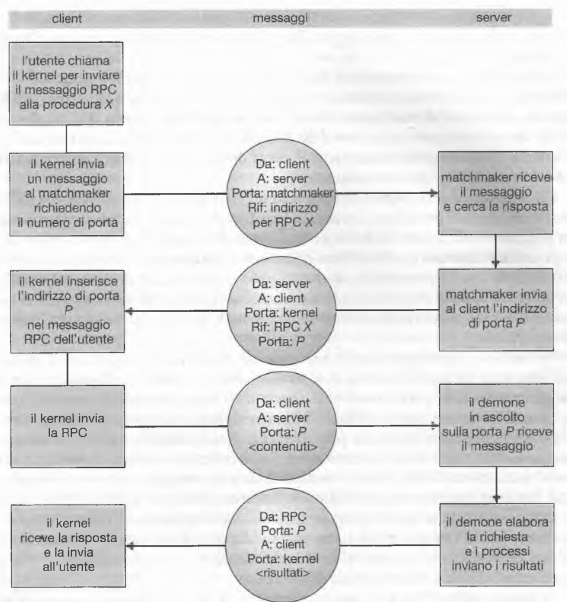
\includegraphics[scale=0.6]{img/0008.png}
\end{center}

\subsubsection{Pipe}
Una pipe\index{pipe} agisce come canale di comunicazione tra processi.\medskip\\
%
\textbf{Pipe convenzionali}\\
Le pipe convenzionali permettono a due processi di comunicare secondo una modalità standard chiamata del produttore-consumatore. Il produttore scrive a una estremità del canale
(\textbf{l'estremità dedicata alla scrittura}, o \emph{write-end}) mentre il consumatore legge dall'altra estre­mità (\textbf{l'estremità dedicata alla lettura}, o \emph{read-end}). Le pipe convenzionali sono quindi unidirezionali. Se viene richiesta la comunicazione a doppio senso devono essere utilizzate due pipe.

Nel sistema UNIX le pipe convenzionali sono costruite utilizzando la funzione \texttt{pipe(int fd[])}.
Essa crea una pipe alla quale si può accedere tramite i descrittori del file \texttt{int fd[]:fd[0]}
è l'estremità dedicata alla lettura, mentre \texttt{fd[1]} è l'estremità dedicata alla scrittura.\\
Non si può accedere a una pipe al di fuori del processo che la crea. Solitamente un pro­cesso padre crea una pipe e la utilizza per comunicare con un processo figlio;
il processo figlio eredita i file
aperti dal processo padre. Dal momento che la pipe è un tipo speciale di file, il figlio eredi­ta la pipe dal proprio processo padre.\medskip\\
%
\textbf{Named pipe}\\
Le pipe convenzionali esistono solo mentre i processi stanno comunican­do. una volta che i processi hanno terminato di comunicare, le
pipe convenzionali cessano di esistere.

Le \textbf{named pipe} costituiscono uno strumento di comunicazione molto più potente; la
comunicazione può essere bidirezionale, e la relazione di parentela padre-figlio non è neces­saria. Una volta che si sia creata la named pipe, diversi processi possono utilizzarla per co­municare. In uno scenario tipico una named pipe ha infatti diversi scrittori. In più, le na­med pipe continuano a esistere anche dopo che i processi comunicanti sono terminati.

Nei sistemi UNIX le named pipe sono dette FIFO. Una volta create, esse appaiono come
normali file all'interno del file system. Una FIFO viene creata mediante una chiamata di siste­
ma \texttt{mkfifo()} e viene poi manipolata con le usuali chiamate di sistema \texttt{open()}, \texttt{read()}, \texttt{write()} e \texttt{close()}; essa continuerà a esistere finché non sarà esplicitamente eliminata dal
file system. Nonostante i file FIFO permettano la comunicazione bidirezionale, l'unica tipolo­gia di trasmissione consentita è quella half duplex\footnote{Trasmissione bidirezionale alternata.}. Nel caso in cui i dati debbano viaggiare in
entrambe le direzioni, vengono solitamente utilizzate due FIFO. Per utilizzare le FIFO i pro­cessi comunicanti devono risiedere sulla stessa macchina: se è richiesta la comunicazione tra
più macchine devono essere impiegate le socket.

Le named pipe su un sistema Windows offrono
un meccanismo di comunicazione più ricco. È permessa la comunicazione full duplex\footnote{Trasmissione bidirezionale simultanea.} e i processi comunicanti possono risiedere sia sulla stessa macchina sia su macchine diverse.
\begin{center}
  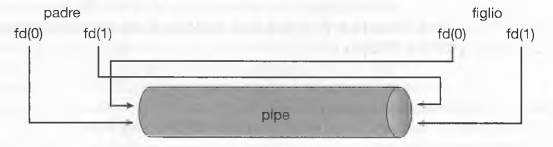
\includegraphics[scale=0.6]{img/0009.png}
\end{center}

\section{Thread}
Molti sistemi operativi moderni permettono
che un processo possa avere più percorsi di controllo che comunemente si chiamano thread.\index{thread}

\subsection{Introduzione}
Un thread è l'unità di base d'uso della CPU e comprende un identificatore di thread (ID), un
contatore di programma, un insieme di registri, e una pila (stack). Condivide con gli altri
thread che appartengono allo stesso processo la sezione del codice, la sezione dei dati e altre
risorse di sistema, come i file aperti e i segnali. Un processo tradizionale, chiamato anche
processo pesante (\emph{heavyweight process})\index{heavyweight process}, è composto da un solo thread. Un processo multi­thread è in grado di lavorare a più compiti in modo concorrente.
\begin{center}
  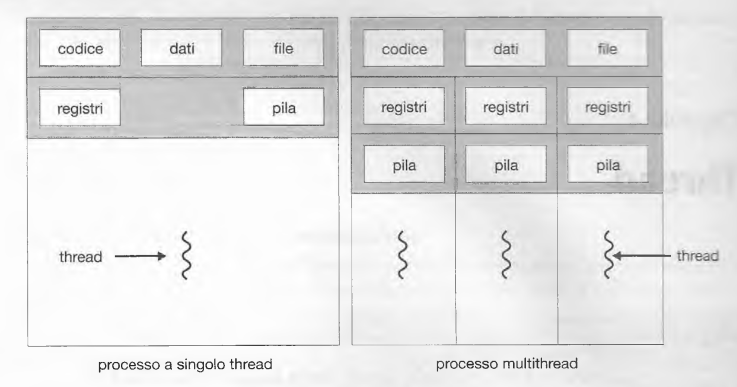
\includegraphics[scale=0.45]{img/0010.png}\\
  \caption{Differenza tra un processo tradizionale, a singolo thread, e uno multithread.}
\end{center}
Di solito, un'applicazione si codifica come un processo a sé stante comprendente
più thread di controllo.

In alcune situazioni, una singola applicazione deve poter gestire molti compiti simili tra lo­ro. Per esempio, per un noto server Web potrebbero esservi molti (forse centinaia) client che vi acce­dono in modo concorrente; se il server Web fosse eseguito come un processo tradizionale a
singolo thread, sarebbe in grado di soddisfare un solo client alla volta. Una soluzione è eseguire il server come un singolo processo che accetta richieste.
Quando ne riceve una, il server crea un processo separato per eseguirla.

La creazione dei processi è molto onerosa, sia a livello dei tempi sia dei co­sti.

Generalmente, per
raggiungere lo stesso obiettivo è più conveniente impiegare un processo multithread:
il server genererebbe un thread distinto per ricevere eventuali richieste dei client;
alla presenza di una richiesta, anziché creare un altro processo, si creerebbe un altro thread
per soddisfarla.
\begin{center}
  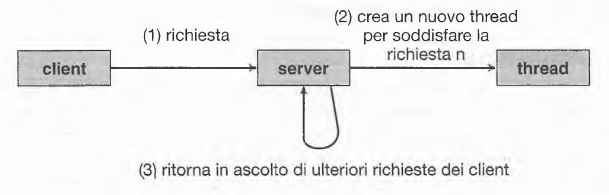
\includegraphics[scale=0.45]{img/0011.png}
\end{center}
Infine, molti kernel di sistemi operativi sono ormai multhithread, con i singoli thread
dedicati a specifici servizi.\medskip\\
\textbf{Vantaggi}\\
- Tempo di risposta;\\
- Condivisione delle risorse;\\
- Economia;\\
- Scalabilità.

\subsubsection{Programmazione multicore}
Una tendenza recente nel progetto dell'architettura dei sistemi consiste nel montare diverse
unità di calcolo (core)\index{core} su un unico processore (un processore multicore\index{multicore}); ogni unità appare al
sistema operativo come un processore separato.

Si consideri un'applicazione con quattro thread. In un sistema
con una singola unità di calcolo “esecuzione concorrente”\footnote{Un sistema concorrente è semplicemente un sistema che gestisce molteplici thread/processi consentendo a tutti di proseguire nell'esecuzione; ciò può avvenire in parallelo su più core o avvicendandosi nell'utilizzo di una CPU.}\index{esecuzione concorrente} significa solo che l'esecuzione dei
thread è stratificata nel tempo, o come anche si dice, interfogliata (\emph{interleaved}),\index{interleaved}
perché la CPU è in grado di eseguire un solo thread alla volta. Su un sistema multicore, inve­ce, “esecuzione concorrente” significa che i thread possono funzionare in parallelo, dal mo­mento che il sistema può assegnare thread diversi a ciascuna unità di calcolo.

\subsection{Modelli di programmazione multithread}
I thread possono essere distinti in thread a livello utente e thread a livello kernel: i primi so­no gestiti senza l'aiuto del kernel; i secondi, invece, sono gestiti direttamente dal sistema
operativo.

\subsubsection{Modello da molti a uno}
II modello da molti a uno fa corrispondere molti thread a livello utente a un
singolo thread a livello kernel. Poiché si svolge nello spazio utente, la gestione dei thread ri­sulta efficiente, ma l'intero processo rimane bloccato se un thread invoca una chiamata di si­stema di tipo bloccante. Poiché un solo thread alla volta può accedere al kernel, è
impossibile eseguire thread multipli in parallelo in sistemi multiprocessore.
\begin{center}
  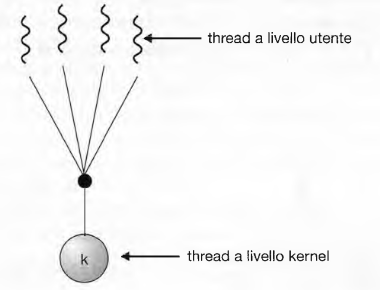
\includegraphics[scale=0.45]{img/0012.png}
\end{center}

\subsubsection{Modello da uno a uno}
Il modello da uno a uno  mette in corrispondenza ciascun thread a livello uten­te con un thread a livello kernel.
Anche se un thread invoca una chiamata di sistema bloccante, è
possibile eseguire un altro thread; il modello permette anche l'esecuzione dei thread in pa­rallelo nei sistemi multiprocessore. L'unico svantaggio di questo modello è che la creazione
di ogni thread a livello utente comporta la creazione del corrispondente thread a livello ker­nel. Poiché il carico dovuto alla creazione di un thread a livello kernel può compromettere le
prestazioni di un'applicazione, la maggior parte delle realizzazioni di questo modello limita
il numero di thread gestibili dal sistema.
\begin{center}
  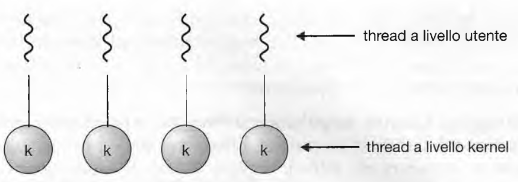
\includegraphics[scale=0.45]{img/0013.png}
\end{center}

\subsubsection{Modello da molti a molti}
Il modello da molti a molti mette in corrispondenza più thread a livello utente
con un numero minore o uguale di thread a livello kernel.
Non viene garantita una concorrenza reale, poiché il meccanismo di scheduling del kernel
può scegliere un solo thread alla volta.
I pro­grammatori possono creare liberamente i thread che ritengono necessari, e i corrispondenti
thread a livello kernel si possono eseguire in parallelo nelle architetture multiprocessore.
Inoltre, se un thread impiega una chiamata disistema bloccante, il kernel può fare in modo
che si esegua un altro thread.

\subsection{Librerie dei thread}
La libreria dei thread fornisce al programmatore una API\index{API} per la creazione e la gestione dei
thread. I metodi con cui implementare una libreria dei thread sono essenzialmente due.

Nel primo, la libreria è collocata interamente a livello utente, senza fare ricorso al kernel. Il co­dice e le strutture dati per la libreria risiedono tutti nello spazio degli utenti. Questo impli­ca che invocare una funzione della libreria si traduce in una chiamata locale a una funzione
nello spazio degli utenti e non in una chiamata di sistema.

Il secondo metodo consiste nell'implementare una libreria a livello kernel, con l'ausi­lio diretto del sistema operativo. In questo caso, il codice e le strutture dati per la libreria si
trovano nello spazio del kernel. Invocare una funzione della API per la libreria provoca, ge­neralmente, una chiamata di sistema al kernel.

Attualmente, sono tre le librerie di thread maggiormente in uso: Pthreads di POSIX,\index{Pthreads}
Win32 e Java.

\subsubsection{Pthreads}
Col termine \textbf{Pthreads}\index{Pthreads} ci si riferisce allo standard POSIX (IEEE 1003.1c) che definisce la API
per la creazione e la sincronizzazione dei thread. Non si tratta di una realizzazione, ma di
una definizione del comportamento dei thread; i progettisti di sistemi operativi possono rea­lizzare le API così definite come meglio credono.

Tutti i programmi che impiegano la libreria Pthreads devono includere il file d'intesta­zione \texttt{pthread.h}. La dichiarazione di variabili \texttt{pthread\_t tid} specifica l'identificatore per
il thread da creare. Ogni thread ha un insieme di attributi che includono la dimensione della
pila e informazioni di scheduling. La dichiarazione \texttt{pthread\_attr\_t attr} riguarda la strut­tura dati per gli attributi del thread, i cui valori si assegnano con la chiamata di funzione \texttt{pthread\_attr\_init(\&attr)}.
La chiamata di funzione\texttt{pthread\_create} crea un
nuovo thread.
Dopo aver creato il secondo, il pri­mo thread attende il completamento del secondo chiamando la funzione \texttt{pthread\_join()}.
Il secondo thread termina quando s'invoca la funzione \texttt{pthread\_exit()}.

\subsubsection{Thread Java}
Il linguaggio Java, con la propria API, è provvisto di una ricca gamma di caratte­ristiche per la generazione e la gestione dei thread. Tutti i programmi scritti in Java incorpo­rano almeno un thread di controllo, costituito soltanto
da un metodo \texttt{main()}, è eseguito dalla JVM come un singolo thread.

In un programma Java vi sono due tecniche per la generazione dei thread. Una è crea­re una nuova classe derivata dalla classe Thread\index{Thread} e “sovrascrivere” (\emph{override}) il suo metodo
\texttt{run()}\index{run()}. L'alternativa, usata più comunemente, consiste nella definizione di una classe che
implementi l'interfaccia \texttt{Runnable}\index{Runnable}.
\begin{center}
  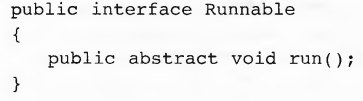
\includegraphics[scale=0.5]{img/0014.png}
\end{center}
La creazione di un oggetto di classe Thread non equivale a generare un nuovo thread:
è il metodo \texttt{start()}\index{start} che avvia effettivamente il nuovo thread. L'invocazione del metodo
\texttt{start()} ha il duplice effetto di:
\begin{enumerate}[noitemsep, leftmargin=*]
  \item allocare la memoria e inizializzare un nuovo thread nella JVM;
  \item chiamare il metodo \texttt{run()}, cosa che rende il thread eseguibile dalla JVM.
\end{enumerate}
Si osservi co­me il metodo \texttt{run()} non sia mai chiamato per via diretta, ma solo tramite la media­zione di \texttt{start()}.

\subsection{Questioni di programmazione multithread}
\subsubsection{Chiamate di sistema fork() e exec()}
In un programma multi­thread la semantica delle chiamate di sistema \texttt{fork()}\index{fork()} e \texttt{exec()}\index{exec()} cambia: se un thread in un programma invoca la chiamata di sistema \texttt{fork()}, il nuovo processo potrebbe, in gene­rale, contenere un duplicato di tutti i thread oppure del solo thread invocante.
Alcuni sistemi UNIX includono entrambe le versioni.

L'uso delle due versioni della \texttt{fork()} dipende dall'applicazione. Se s'invoca la
\texttt{exec()} immediatamente dopo la \texttt{fork()}, la duplicazione dei thread non è necessaria, poi­ché il programma specificato nei parametri della \texttt{exec()} sostituirà il processo. In questo ca­so conviene duplicare il solo thread chiamante. Tuttavia, se la \texttt{exec()} non segue immedia­tamente la \texttt{fork()}, potrebbe essere utile una duplicazione di tutti i thread del processo ge­nitore.

\subsubsection{Cancellazione}
La cancellazione dei thread è l'operazione che permette di terminare un thread prima che
completi il suo compito.
Un thread da cancellare è spesso chiamato \textbf{thread bersaglio} (\emph{target thread}).\index{target thread} La cancel­lazione di un thread bersaglio può avvenire in due modi diversi:
\begin{enumerate}[noitemsep, leftmargin=*]
  \item \textbf{cancellazione asincrona}. Un thread fa immediatamente terminare il thread bersaglio;
  \item \textbf{cancellazione differita}. Il thread bersaglio può periodicamente controllare se deve ter­minare, in modo da riuscirvi in modo opportuno.
\end{enumerate}
Si presentano difficoltà con la cancellazione nei casi in cui ci siano risorse assegnate a un thre­ad cancellato, o se si cancella un thread mentre sta aggiornando dei dati che condivide con al­tri thread.

La cancellazione di un
thread in modo asincrono potrebbe non liberare una risorsa necessaria per tutto il sistema.
La cancellazione differita invece funziona tramite un thread che segnala la necessità di
cancellare un certo thread bersaglio; la cancellazione avviene soltanto quando il thread ber­saglio verifica se debba essere o meno cancellato. Questo metodo permette di programmare
la verifica in un punto dell'esecuzione in cui il thread sia cancellabile senza problemi. Nella
libreria Pthreads questi punti si chiamano \textbf{punti di cancellazione} (\emph{cancellation point}).\index{cancellation point}

\subsubsection{Gestione dei segnali}
Nei sistemi UNIX si usano i segnali per comunicare ai processi il verificarsi di determinati
eventi. Un segnale si può ricevere in modo sincrono o asincrono, secondo la sorgente e la ra­gione della segnalazione dell'evento. Indipendentemente dal modo di ricezione sincrono o
asincrono, tutti i segnali seguono lo stesso schema:
\begin{enumerate}[noitemsep, leftmargin=*]
  \item all'occorrenza di un particolare evento si genera un segnale;
  \item s'invia il segnale a un processo;
  \item una volta ricevuto, il segnale deve essere gestito.
\end{enumerate}
Quando un segnale è causato da un evento esterno al processo in esecuzione, tale pro­cesso riceve il segnale in modo asincrono. Ad esempio <control><C>
oppure la scadenza di un timer. Di solito un segnale asincrono s'invia a un altro processo. Ogni segnale si può gestire in due modi:
\begin{enumerate}[noitemsep, leftmargin=*]
  \item tramite un gestore predefinito di segnali;
  \item tramite un gestore di segnali definito dall'utente.
\end{enumerate}
Per ogni segnale esiste un gestore predefinito del segnale che il kernel esegue quando deve
gestire il segnale. La gestione predefinita è sostituibile da una funzione di gestione del se­gnale definita dall'utente, richiamata per gestire il segnale.

La funzione UNIX per recapitare i segnali è \texttt{kill(aid\_t aid, int signal)}, dove aid specifica il processo a cui recapitare il segnale \texttt{signal}. La
API Pthreads POSIX, però, dispone anche della funzione \texttt{pthread\_kill(pthread\_t tid, int signal)} che permette di specificare il thread (\texttt{tid}) cui recapitare il segnale.

Sebbene Windows non preveda la gestione esplicita dei segnali, questi si possono emu­lare con le \textbf{chiamate di procedure asincrone}\index{chiamate di procedure asincrone} (\emph{asynchronous procedure call}, APC\index{APC}). Le funzioni
APC permettono a un thread a livello utente di specificare la funzione da richiamare quando
il thread riceve la comunicazione di un particolare evento.

\subsubsection{Gruppi di thread}
Un numero illimitato di thread potrebbe esaurire le risorse del sistema,
come il tempo di CPU o la memoria. L'impiego dei gruppi di thread (\emph{thread pool})\index{thread pool} è una pos­sibile soluzione a questo problema.

L'idea generale è quella di creare un certo numero di thread alla creazione del proces­so, e organizzarli in un gruppo (\emph{pool}) in cui attendano il lavoro che gli sarà richiesto.

\subsubsection{Dati specifici dei thread}
Uno dei vantaggi principali della programmazione multithread è dato dal fatto che i thread
appartenenti allo stesso processo ne condividono i dati. Tuttavia, in particolari circostanze,
ogni thread può necessitare di una copia privata di certi dati, chiamati \textbf{dati specifici di
thread}.

\subsubsection{Attivazione dello scheduler}
Molti sistemi che implementano o il modello da molti a molti o quello a due livelli
collocano una struttura dati intermedia tra i thread del kernel e dell'utente, nota come processo leggero o LWP\index{LWP} (\emph{Lightweight Process})\index{light weight process}. Essa si presenta co­me un processore virtuale a cui l'applicazione può richiedere lo scheduling di un thread a li­vello dell'utente. Ciascun LWP è associato a un thread del kernel, e sono proprio i thread del
kernel che il sistema operativo pone in esecuzione sui processori fisici. Se un thread del ker­nel si arresta anche
LWP si blocca. L'effetto a catena risale fino al thread a livello utente associato a LWP, che si
blocca anch'esso.

Di solito, è necessario un LWP per ogni chiamata di sistema concorrente
bloccante.
Uno dei modelli di comunicazione tra la libreria a livello utente e il kernel è conosciu­to come \textbf{attivazione dello scheduler}\index{attivazione dello scheduler}. Il suo funzionamento è il seguente: il kernel fornisce
all'applicazione una serie di processori virtuali (LWP), mentre l'applicazione esegue lo sche­duling dei thread dell'utente sui processori virtuali disponibili. Inoltre, il kernel deve infor­mare l'applicazione se si verificano determinati eventi, seguendo una procedura nota come
\textbf{upcall}.\index{upcall}
Il gestore di questa upcall necessita anch'esso di un processore virtuale: il
kernel può crearne uno ex novo, o sottrarlo a un thread utente per prelazione.

\section{Scheduling della CPU}
Attraverso la
commutazione del controllo della CPU tra i vari processi, il sistema operativo può rendere
più produttivo il calcolatore.

\subsection{Concetti fondamentali}
In un sistema monoprocessore si può eseguire al massimo un processo alla volta; gli altri
processi, se ci sono, devono attendere che la CPU sia libera e possa essere nuovamente sotto­
posta a scheduling.

Un processo è in esecu­zione finché non deve attendere un evento; durante l'attesa,
la CPU resterebbe inattiva. Con la multiprogrammazione si cerca d'impiega­re questi tempi d'attesa in modo produttivo: si tengono contemporaneamente più processi
in memoria, e quando un processo deve attendere un evento, il sistema operativo gli sottrae
il controllo della CPU per cederlo a un altro processo.

\subsubsection{Ciclicità delle fasi d'elaborazione e di I/O}
L'esecuzione del processo consiste in un ciclo d'elaborazione (svolta dalla CPU) e
d'attesa del completamento delle operazioni di I/O. L'esecuzione di un processo comincia con una sequenza (una "raffica") di operazioni
d'elaborazione svolte dalla CPU (\emph{CPU burst}),\index{CPU burst} seguita da una sequenza di operazioni di I/O
(\emph{I/O burst}),\index{I/O burst} \index{burst} quindi un'altra sequenza di operazioni della CPU, di nuovo una sequenza di ope­razioni di I/O, e così via.

La loro curva di frequenza è generalmente di tipo esponenziale o iperesponenziale, con molte brevi sequenze di operazioni della CPU, e poche sequenze di operazioni della
CPU molto lunghe. Un programma con prevalenza di I/O (\emph{I/O bound})\index{I/O bound} produce generalmen­te molte sequenze di operazioni della CPU di breve durata. Un programma con prevalenza
d'elaborazione (\emph{CPU bound}),\index{CPU bound} \index{bound} invece, produce poche sequenze di operazioni della CPU molto
lunghe. Queste caratteristiche possono essere utili nella scelta di un appropriato algoritmo
di scheduling della CPU.

\subsubsection{Scheduler della CPU}
Ogniqualvolta la CPU passa nello stato d'inattività, il sistema operativo sceglie per l'esecuzione uno dei processi presenti nella coda dei processi pronti. È lo \textbf{scheduler
a breve termine},\index{scheduler
a breve termine} o scheduler della CPU che, tra i processi in memoria pronti per l'esecuzio­ne, sceglie quello cui assegnare la CPU.
La coda dei processi pronti non è necessariamente FIFO.
Gene­ralmente gli elementi delle code sono i \emph{process control block}\index{process control block} (PCB)\index{PCB} dei processi.

\subsubsection{Scheduling con diritto di prelazione}
Le decisioni riguardanti lo scheduling della CPU si possono prendere nelle seguenti circo­stanze:
\begin{enumerate}[noitemsep, leftmargin=*]
  \item un processo passa dallo stato di esecuzione allo stato di attesa,
  \item un processo passa dallo stato di esecuzione allo stato pronto,
  \item un processo passa dallo stato di attesa allo stato pronto,
  \item un processo termina.
\end{enumerate}
Quando lo scheduling interviene solo nelle condizioni 1 e 4, si dice che lo schema di
scheduling è \textbf{senza diritto di prelazione}\index{prelazione}\index{diritto di prelazione} (\emph{nonpreemptive}) o \textbf{cooperativo} (\emph{cooperative}); altri­menti, lo schema di scheduling è \textbf{con diritto di prelazione} (\emph{preemptive}).

Sfortunatamente lo scheduling con diritto di prelazione presenta un inconveniente. Si
consideri il caso in cui due processi condividono dati; mentre uno di questi aggiorna i dati
si ha la sua prelazione in favore dell'esecuzione dell'altro. Il secondo processo può, a questo
punto, tentare di leggere i dati che sono stati lasciati in uno stato incoerente dal primo pro­cesso. Sono quindi necessari nuovi meccanismi per coordinare l'accesso ai dati condivisi;

\subsubsection{Dispatcher}
Un altro elemento coinvolto nella funzione di scheduling della CPU è il \textbf{dispatcher};\index{dispatcher} si tratta
del modulo che passa effettivamente il controllo della CPU ai processi scelti dallo scheduler
a breve termine. Questa funzione riguarda quel che segue:
\begin{itemize}[noitemsep, leftmargin=*]
  \item il cambio di contesto;
  \item il passaggio alla modalità utente;
  \item il salto alla giusta posizione del programma utente per riavviarne l'esecuzione.
\end{itemize}
%
Poiché si attiva a ogni cambio di contesto, il dispatcher dovrebbe essere quanto più rapido è
possibile. Il tempo richiesto dal dispatcher per fermare un processo e avviare l'esecuzione di
un altro è nota come \textbf{latenza di dispatch}.\index{latenza}

\subsection{Criteri di scheduling}
- Utilizzo della CPU\\
- Produttività\\
- Tempo di completamento\\
- Tempo d'attesa\\
- Tempo di risposta\\

\subsection{Algoritmi di scheduling}
\subsubsection{Scheduling in ordine d'arrivo}
Il più semplice algoritmo di scheduling della CPU è l'algoritmo di \textbf{scheduling in ordine d'ar­rivo} (\emph{scheduling first-come, first-served}, FCFS.\index{FCFS} La realizzazione del criterio FCFS si fonda su una coda FIFO.
Il tempo medio d'attesa per l'algoritmo FCFS è spesso abbastanza lungo.\medskip\\
Si consideri il seguente esempio:
\begin{center}
  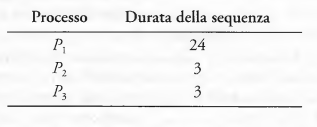
\includegraphics[scale=0.6]{img/0015.png}
\end{center}
Se i processi arrivano nell'ordine $P_1$, $P_2$, $P_3$ sono serviti in ordine FCFS, si ottiene il risulta­to illustrato dal seguente nel seguente \textbf{diagramma di Gantt}:\index{Gantt}
\begin{center}
  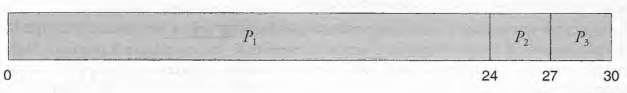
\includegraphics[scale=0.5]{img/0016.png}
\end{center}
Il tempo d'attesa è 0 millisecondi per il processo $P_1$, 24 millisecondi per il processo $P_2$ e 27
millisecondi per il processo $P_3$. Quindi, il tempo d'attesa medio è (0 + 24 + 27)/3 = 17 millisecondi. Se i processi arrivassero nell'ordine $P_2$, $P_3$, $P_1$, i risultati sarebbero quelli illustrati nel seguente diagramma di Gantt:
\begin{center}
  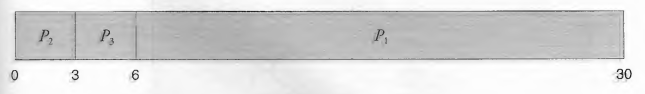
\includegraphics[scale=0.5]{img/0017.png}
\end{center}
Il tempo di attesa medio è ora di (6 + 0 + 3)/3 = 3 millisecondi.\medskip\\
Si considerino inoltre le prestazioni dello scheduling FCFS in una situazione dinamica.
Si supponga di avere un processo con prevalenza d'elaborazione e molti processi con preva­lenza di i/o. Via via che i processi fluiscono nel sistema si può riscontrare come il processo
con prevalenza d'elaborazione occupi la CPU. Durante questo periodo tutti gli altri processi
terminano le proprie operazioni di I/O e si spostano nella coda dei processi pronti, nell'atte­sa della CPU. Mentre i processi si trovano nella coda dei processi pronti, i dispositivi di I/O
sono inattivi. Successivamente il processo con prevalenza d'elaborazione termina la propria
sequenza di operazioni della CPU e passa a una fase di I/O. Tutti i processi con prevalenza di
I/O, caratterizzati da sequenze di operazioni della CPU molto brevi, sono eseguiti rapida­mente e tornano alle code di I/O, lasciando inattiva la CPU. Il processo con prevalenza d'ela­borazione torna nella coda dei processi pronti e riceve il controllo della CPU; così, finché
non termina l'esecuzione del processo con prevalenza d'elaborazione, tutti i processi con
prevalenza di I/O si trovano nuovamente ad attendere nella coda dei processi pronti. Si ha
un \textbf{effetto convoglio}, tutti i processi attendono che un lungo processo liberi la CPU, che causa una riduzione dell'utilizzo della CPU e dei dispositivi rispetto a quella che si avrebbe se si
eseguissero per primi i processi più brevi.\medskip\\
L'algoritmo di scheduling FCFS è senza prelazione.

\subsubsection{Scheduling per brevità}
Un criterio diverso di scheduling della CPU si può ottenere con l'algoritmo di \textbf{scheduling
per brevità} (\emph{shortest-job-first}, SJF).\index{SJF} Questo algoritmo associa a ogni processo la lunghezza
della successiva sequenza di operazioni della CPU. Quando è disponibile, si assegna la CPU al
processo che ha la più breve lunghezza della successiva sequenza di operazioni della CPU. Se
due processi hanno le successive sequenze di operazioni della CPU della stessa lunghezza si
applica lo scheduling FCFS.\medskip\\
Si consideri ad esempio:
\begin{center}
  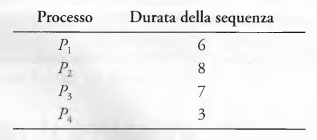
\includegraphics[scale=0.6]{img/0018.png}
\end{center}
Con lo scheduling SJF questi processi si ordinerebbero secondo il seguente diagramma di
Gantt:
\begin{center}
  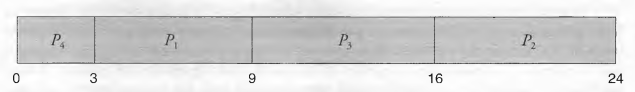
\includegraphics[scale=0.5]{img/0019.png}
\end{center}
Si può dimostrare che l'algoritmo di scheduling SJF è \emph{ottimale}, nel senso che rende mi­nimo il tempo d'attesa medio per un dato insieme di processi. Spostando un processo breve
prima di un processo lungo, il tempo d'attesa per il processo breve diminuisce più di quan­to aumenti il tempo d'attesa per il processo lungo. Di conseguenza, il tempo d'attesa \emph{medio}
diminuisce.\medskip\\
Sebbene sia ottimale, l'algoritmo SJF non si può realizzare a livello dello scheduling
della CPU a breve termine, poiché non esiste alcun modo per conoscere la lunghezza della
successiva sequenza di operazioni della CPU. Un possibile metodo consiste nel tentare di ap­prossimare lo scheduling SJF: se non è possibile \emph{conoscere} la lunghezza della prossima se­quenza di operazioni della CPU, si può cercare di \emph{predire} il suo valore.\medskip\\
La lunghezza della successiva sequenza di operazioni della CPU generalmente si ottiene
calcolando la media esponenziale delle effettive lunghezze delle precedenti sequenze di ope­razioni della CPU. La media esponenziale si definisce con la formula seguente:\\
$t_n$ lunghezza dell'$n$-esima sequenza di operazioni della CPU\\
$\tau_{n+1}$ valore previsto
per la successiva sequenza di operazioni della CPU\\
$\alpha$ tale che $0 <= \alpha <= 1$\\
\[ \tau_{n+1}=t_n+(1-\alpha)\tau_n \]
Il valore di $t_n$ contiene le informazioni più recenti; $\tau_n$ registra la storia passata. Il parametro $\alpha$ controlla il peso relativo sulla predizione della storia recente e di quella passata. Se $\alpha = 0$,
allora, $_{n+1}=\tau_n$, e la storia recente non ha effetto; si suppone, cioè, che le condizioni attuali
siano transitorie; se $\alpha=1$, allora $\tau_{n+1}=t_n$, e ha significato solo la più recente sequenza di ope­razioni della CPU: si suppone, cioè, che la storia sia vecchia e irrilevante. Più comune è la
condizione in cui $\alpha=\frac{1,2}$, valore che indica che la storia recente e la storia passata hanno lo
stesso peso.\medskip\\
L'algoritmo SJF può essere sia \emph{con prelazione} sia \emph{senza prelazione}. La scelta si presenta
quando alla coda dei processi pronti arriva un nuovo processo mentre un altro processo è
ancora in esecuzione. Il nuovo processo può avere una successiva sequenza di operazioni del­la CPU più breve di quella che resta al processo correntemente in esecuzione. Un algoritmo
SJF con prelazione sostituisce il processo attualmente in esecuzione, mentre un algoritmo SJF
senza prelazione permette al processo correntemente in esecuzione di portare a termine la
propria sequenza di operazioni della CPU. (Lo scheduling SJF con prelazione è talvolta chia­mato scheduling \emph{shortest-remaining-time-first}).\medskip\\
Condsideriamo il seguente esempio. Dallo scheduling SJF con prelazione ri­sulta:
\begin{center}
  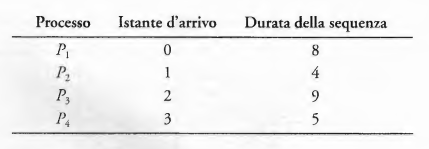
\includegraphics[scale=0.6]{img/0020.png}\medskip\\
  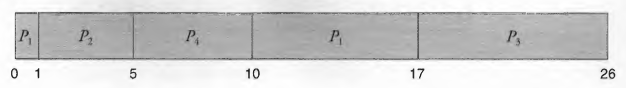
\includegraphics[scale=0.5]{img/0021.png}
\end{center}
Il tempo d'attesa medio per questo esempio è
((10 - 1) + (1 - 1) + (17 - 2) + (5 - 3))/4 = 26/4 = 6,5 millisecondi.\\
Con uno scheduling
SJF senza prelazione si otterrebbe un tempo d'attesa medio di 7,75 millisecondi.\\

\subsubsection{Scheduling per priorità}
L'algoritmo SJF è un caso particolare del più generale algoritmo di scheduling per priorità:
si associa una priorità a ogni processo e si assegna la CPU al processo con priorità più alta; i
processi con priorità uguali si ordinano secondo uno schema FCFS.\\
A una maggiore lunghezza corrispon­de una minore priorità, e viceversa.

Occorre notare che la discussione si svolge nei termini di priorità alta e priorità bassa.
Generalmente le priorità sono indicate da un intervallo fisso di numeri, come da 0 a 7, oppure da 0 a 4,095. Tuttavia, non si è ancora stabilito se attribuire allo 0 la priorità più alta o
quella più bassa; alcuni sistemi usano numeri bassi per rappresentare priorità basse, altri usa­
no numeri bassi per priorità alte.

Le priorità si possono definire sia internamente sia esternamente. Quelle definite in­ternamente usano una o più quantità misurabili per calcolare la priorità del processo; per
esempio, i limiti di tempo, i requisiti di memoria, il numero dei file aperti e il rapporto tra
la lunghezza media delle sequenze di operazioni di I/O e la lunghezza media delle sequenze
di operazioni della CPU. Le priorità esterne si definiscono secondo criteri esterni al sistema
operativo, come l'importanza del processo, il tipo e la quantità dei fondi pagati per l'uso del
calcolatore, il dipartimento che promuove il lavoro e altri fattori, spesso di ordine politico.

Un problema importante relativo agli algoritmi di scheduling per priorità è l'attesa in­definita (\emph{starvation}, letteralmente, "inedia"). Un processo pronto per l'esecuzione, ma che
non dispone della CPU, si può considerare bloccato nell'attesa della CPU. Un algoritmo di
scheduling per priorità può lasciare processi con bassa priorità nell'attesa indefinita della
CPU. Un flusso costante di processi con priorità maggiore può impedire a un processo con
bassa priorità di accedere alla CPU. Generalmente accade che o il processo è eseguito quando il sistema ha finalmente ridotto il proprio carico, op­pure il calcolatore si sovraccarica al punto da perdere tutti i processi con bassa priorità non
terminati. Corre voce che, quando fu fermato l'IBM 7094 al MIT, nel 1973, si scoprì che un
processo con bassa priorità sottoposto nel 1967 non era ancora stato eseguito.

Una soluzione al problema dell'attesa indefinita dei processi con bassa priorità è costi­
tuita dall'invecchiamento (\emph{aging}); si tratta di una tecnica di aumento graduale delle priorità
dei processi che attendono nel sistema da parecchio tempo.

\subsubsection{Scheduling circolare}
L'\textbf{algoritmo di scheduling circolare} (\emph{round-robin}, \index{round-robin} RR\index{RR}) è stato progettato appositamente per
i sistemi a tempo ripartito; simile allo scheduling FCFS, ha tuttavia in più la capacità di pre­
lazione per la commutazione dei processi. Ciascun processo riceve una piccola quantità fis­
sata del tempo della CPU, chiamata \textbf{quanto di tempo} o porzione di tempo (\emph{time slice}),\index{time slice} che
varia generalmente da 10 a 100 millisecondi; la coda dei processi pronti è trattata come una
coda circolare. Lo scheduler della CPU scorre la coda dei processi pronti, assegnando la CPU
a ciascun processo per un intervallo di tempo della durata massima di un quanto di tempo.

Si gestisce la coda dei processi pronti come una coda FI­FO. I nuovi processi si aggiungono alla fine della coda dei processi pronti. Lo scheduler del­la CPU individua il primo processo dalla coda dei processi pronti, imposta un timer in mo­do che invii un segnale d'interruzione alla scadenza di un intervallo pari a un quanto di tem­po, e attiva il dispatcher per l'effettiva esecuzione del processo.

A questo punto si può verificare una delle seguenti situazioni: il processo ha una se­quenza di operazioni della CPU di durata minore di un quanto di tempo, quindi il processo
stesso rilascia volontariamente la CPU e lo scheduler passa al processo successivo della coda
dei processi pronti; oppure la durata della sequenza di operazioni della CPU del processo attualmente in esecuzione è più lunga di un quanto di tempo; in questo caso si raggiunge la
scadenza del quanto di tempo e il timer invia un segnale d'interruzione al sistema operativo,
che esegue un cambio di contesto, aggiunge il processo alla fine della coda dei processi pron­ti e, tramite lo scheduler della CPU, seleziona il processo successivo nella coda dei processi
pronti. Il tempo d'attesa medio per il criterio di scheduling RR è spesso abbastanza lungo.

Nell'algoritmo di scheduling RR la CPU si assegna a un processo per non più di un
quanto di tempo per volta. Se la durata della sequenza di operazioni della CPU di un proces­so eccede il quanto di tempo, il processo viene sottoposto a prelazione e riportato nella coda
dei processi pronti. L'algoritmo di scheduling RR è pertanto con prelazione.

Se nella coda dei processi pronti esistono n processi e il quanto di tempo è pari a $q$, ciascun processo ottiene $1/n$-esimo del tempo di elaborazione della CPU in frazioni di, al mas­simo, $q$ unità di tempo. Ogni processo non deve attendere per più di $(n-1)\times q$ unità di
tempo.

Le prestazioni dell'algoritmo RR dipendono molto dalla dimensione del quanto di
tempo. Nel caso limite in cui il quanto di tempo sia molto lungo (indefinito), il criterio di
scheduling RR si riduce al criterio di scheduling FCFS. Se il quanto di tempo è molto breve
(per esempio, un microsecondo), il criterio RR si chiama \textbf{condivisione della CPU} (\emph{processor
sharing}) e teoricamente gli utenti hanno l'impressione che ciascuno degli $n$ processi dispon­ga di una propria CPU in esecuzione a $1/n$ della velocità della CPU reale.

Riguardo alle prestazioni dello scheduling RR, occorre tuttavia considerare l'effetto dei
cambi di contesto. Dato un solo processo della durata di 10 unità di tempo, se il quanto di
tempo è di 12 unità, il processo impiega meno di un quanto di tempo; se però il quanto di
tempo è di 6 unità, il processo richiede 2 quanti di tempo e un cambio di contesto; e se il
quanto di tempo è di un'unità di tempo, occorrono nove cambi di contesto, con proporzio­nale rallentamento dell'esecuzione del processo.

\begin{center}
  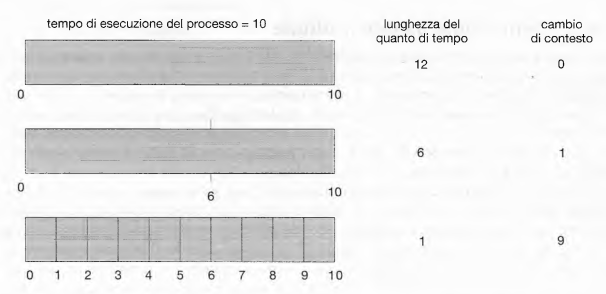
\includegraphics[scale=0.5]{img/0022.png}
\end{center}

\subsubsection{Scheduling a code multiple}
I processi si distinguono in quelli si eseguono in \textbf{primo piano} (\emph{foreground}), o interattivi, e i proces­si che si eseguono in \textbf{sottofondo} (\emph{background}), o a \textbf{lotti} (\emph{batch}). Questi due tipi di processi
hanno tempi di risposta diversi e possono quindi avere diverse necessità di scheduling. Inol­tre, i processi che si eseguono in primo piano possono avere la priorità, definita esterna­mente, sui processi che si eseguono in sottofondo.

L'\textbf{algoritmo di scheduling a code multiple} (\emph{multilevel queue scheduling algorithm}) sud­divide la coda dei processi pronti in code distinte.
I processi si assegnano in mo­do permanente a una coda, secondo qualche caratteristica del processo. Ogni coda ha il proprio algoritmo di scheduling.
La coda dei processi in primo piano si può gestire con un algoritmo FCFS.
In questa situazione è inoltre necessario avere uno scheduling tra le code; si tratta comune­mente di uno scheduling per priorità fissa e con prelazione.

Ogni coda ha la priorità assoluta sulle code di priorità più bassa; nessun processo della coda
dei processi in sottofondo può iniziare l'esecuzione finché le code per i processi prioritari non siano tutte vuote.

Esiste anche la possibilità di impostare i quanti di tempo per le code. Per ogni coda si
stabilisce una parte del tempo d'elaborazione della CPU, suddivisibile a sua volta tra i pro­cessi che la costituiscono.

\subsubsection{Scheduling a code multiple con retroazione}
Di solito in un algoritmo di scheduling a code multiple i processi si assegnano in modo per­manente a una coda all'entrata nel sistema, e non si possono spostare tra le code.

Lo \textbf{scheduling a code multiple con retroazione}\index{retroazione} (\emph{multilevel feedback queue scheduling}),
invece, permette ai processi di spostarsi fra le code.
Se un processo usa troppo tempo di elaborazione della CPU, viene spostato in una coda con priorità più bassa. Si può spostare in una coda con priorità più elevata un processo che attende troppo a lungo.

Generalmente uno scheduler a code multiple con retroazione è caratterizzato dai se­guenti parametri:
\begin{itemize}
  \item numero di code;
  \item algoritmo di scheduling per ciascuna coda;
  \item metodo usato per determinare quando spostare un processo in una coda con priorità maggiore;
  \item metodo usato per determinare quando spostare un processo in una coda con priorità minore;
  \item metodo usato per determinare in quale coda si deve mettere un processo quando ri­chiede un servizio.
\end{itemize}
%
La definizione di uno scheduler a code multiple con retroazione costituisce il più generale
criterio di scheduling della CPU. Sfortunatamente corrisponde anche all'algoritmo più complesso.

\subsection{Scheduling dei thread}
Sui sistemi operativi che prevedono la presenza di thread a \emph{livello utente} e a \emph{livello kernel},
il sistema pianifica l'esecuzione dei thread a livello kernel, non dei processi. I thread a livello utente sono gestiti da una libreria: il kernel non è consapevole della loro esistenza. Di
conseguenza, per eseguire i thread a livello utente occorre associare loro dei thread a livello
kernel. Tale associazione può essere indiretta, ossia realizzata con un processo leggero (LWP).

\subsubsection{Ambito della competizione}
La prima distinzione fra thread a livello utente e a livello kernel riguarda il modo in cui è
pianificata la loro esecuzione. Nei sistemi che impiegano il modello da molti a uno e il modello da molti a molti, la libreria dei thread pianifica
l'esecuzione dei thread a livello utente su un LWP libero; si parla allora di \textbf{ambito della com­petizione ristretto al processo} (\emph{process-contention scope, PCS}).\index{PCS} \index{process contention scope}
Per determinare quale
thread a livello kernel debba essere eseguito da una CPU, il kernel esamina i thread di tutto
il sistema; si parla allora di \textbf{ambito della competizione allargato al sistema} (\emph{system-contention scope, SCS}).
Se l'ambito della competizione è ristretto al processo, lo scheduling è solitamente ba­sato sulle priorità.

\subsubsection{Scheduling di Pthread}
La API Pthread del POSIX consente di specificare sia PCS che SCS per la generazione dei thread.
Per l'ambito della contesa:
\begin{description}[leftmargin=*]
  \item[PTHREAD\_SCOPE\_PROCESS] pianifica i thread con lo scheduling PCS (pianifica i thread a livello utente sugli LWP disponibili. Il nume­ro di LWP viene stabilito dalla libreria dei thread, che in qualche caso si serve delle attivazio­ni dello scheduler).
  \item [PTHREAD\_SCOPE\_SYSTEM] pianifica i thread tramite lo scheduling SCS (crea, in corri­spondenza di ciascun thread a livello utente, un LWP a esso vincolato, realizzando così una corrispondenza secondo il modello da molti a uno).
\end{description}
%
Lo IPC di Pthread offre due funzioni per appurare e impostare l'ambito della contesa:
\begin{itemize}
  \item \texttt{pthread\_attr\_setscope(pthread\_attr\_t *attr, int scope)}
  \item \texttt{pthread\_attr\_getscope(pthread\_attr\_t *attr, int *scope)}
\end{itemize}
Il primo parametro per entrambe le funzioni è un puntatore agli attributi del thread. Il se­condo parametro della funzione pthread\_attr\_setscope() riceve
PTHREAD\_SCOPE\_SYSTEM o PTHREAD\_SCOPE\_PROCESS, che stabiliscono l'ambito della
contesa.\\
Qualora si verifichi un errore, ambedue le funzioni restituiscono valori non nulli.

\subsection{Scheduling per sistemi multiprocessore}
Se sono disponibili più unità d'elaborazione, anche il problema del­lo scheduling è proporzionalmente più complesso.
Consideriamo i sistemi in cui le unità d'elaborazione sono, in
relazione alle loro funzioni, identiche (\textbf{sistemi omogenei}): si può usare qualunque unità
d'elaborazione disponibile per eseguire qualsiasi processo presente nella coda.

\subsubsection{Soluzioni di scheduling per multiprocessori}
Una prima strategia di scheduling della CPU per i sistemi multiprocessore affida tutte le de­cisioni,  a un solo processore, il cosiddet­to \emph{master server}. Gli altri processori eseguono soltanto il codice dell'utente. Si tratta della \textbf{multielaborazione asimmetrica}.\index{multielaborazione asimmetrica}
Quando invece ciascun processore provvede al proprio scheduling, si parla di \textbf{multie­laborazione simmetrica}\index{multielaborazione simmetrica} (\emph{symmetric multiprocessing, SMP}). In questo caso i processi pronti
per l'esecuzione sono situati tutti in una coda comune, oppure vi è un'apposita coda per
ogni processore.

\subsubsection{Predilezione per il processore}
Si consideri che cosa accade alla memoria cache dopo che un processo sia stato eseguito da
uno specifico processore: i dati che il processore ha trattato da ultimo permangono nella ca­che e, di conseguenza, i successivi accessi alla memoria da parte del processo tendono a uti­lizzare spesso la memoria cache.\\
Se un processo si sposta su un
altro processore, i contenuti della memoria cache devono essere invalidati sul processore di
partenza, mentre la cache del processore di arrivo deve essere nuovamente riempita. A causa
degli alti costi di svuotamento e riempimento della cache, molti sistemi SMP tentano di im­pedire il passaggio di processi da un processore all'altro, mirando a mantenere un processo
sullo stesso processore che lo sta eseguendo. Si parla di predilezione\index{predilezione} per il processore (\emph{pro­cessor affinity}).

Quando un sistema opera­tivo si propone di mantenere un processo su un singolo processore, ma non garantisce che
sarà così, si parla di \textbf{predilezione debole} (\emph{soft affinity}).\\
Alcuni sistemi, per esempio Linux, dispongono di
chiamate di sistema con cui specificare che un processo non debba cambiare processore; in
tal modo, si realizza la \textbf{predilezione forte} (\emph{hard affinity}).

\subsubsection{Bilanciamento del carico}
Il bilanciamento del carico tenta di ripartire il carico di lavoro
uniformemente tra tutti i processori di un sistema SMP.
Nei sistemi che mantengono una coda comune, il bilanciamento del carico è sovente superfluo: un processore inattivo passerà immediatamente all'esecuzione di
un processo dalla coda comune eseguibile dei processi.

Il
bilanciamento del carico può seguire due approcci: la \textbf{migrazione guidata}\index{migrazione guidata} (\emph{push migration}) e la \textbf{migrazione spontanea}\index{migrazione spontanea} (\emph{pull migration}). La prima prevede che un processo ap­posito controlli periodicamente il carico di ogni processore; la migrazione spontanea, invece, si ha quando un processore inattivo sottrae
ad un processore sovraccarico un processo in attesa. I due tipi di migrazione non sono mu­tuamente esclusivi, e trovano spesso applicazione contemporanea nei sistemi con bilancia­mento del carico.

\subsubsection{Processori multicore}
La tendenza recente nel progetto di processori è di inse­rire più unità di calcolo in un unico chip fisico, dando origine a un \textbf{processore multicore}\index{multicore}.
I processori multicore possono complicare i problemi relativi allo scheduling.

Quando un
processore accede alla memoria, una quantità significativa di tempo trascorre in attesa della
disponibilità dei dati. Questa situazione, nota come \textbf{stallo della memoria},\index{stallo della memoria} può verificarsi
per varie ragioni.
Il processore può trascorrere fino al 5\% del suo tempo attendendo che i dati siano disponibili in memoria. Per rimediare
a questa situazione, molti dei progetti hardware recenti implementano delle unità di calcolo
multithread in cui due o più thread hardware sono assegnati a una singola unità di calcolo.
In questo modo, se un thread è in situazione di stallo in attesa della memoria, l'unità di cal­colo può passare il controllo a un altro thread.

In generale, ci sono due modi per rendere un processore multithread: attraverso il \textbf{multithreading grezzo} (\emph{coarse-grained}) o il \textbf{multithreading fine}\index{multithreading} (\emph{fine-grained}). Nel multithreading grezzo un thread resta in esecuzione su un processore fino al verificarsi di un evento a lunga latenza, come ad esempio uno stallo di memoria. A causa dell'attesa introdotta dal­l'evento a lunga latenza, il processore deve passare a un altro thread e iniziare a eseguirlo. Tut­tavia, il costo per cambiare il thread in esecuzione è alto, perché occorre ripulire la pipeline
delle istruzioni prima che il nuovo thread possa iniziare a essere eseguito sull'unità di calcolo.
Quando il nuovo thread è in esecuzione inizia a riempire la pipeline con le sue istruzioni. Il
multithreading fine (anche detto \emph{multithreading interfogliato}) passa da un thread a un altro
con un livello molto più fine di granularità (tipicamente al termine di un ciclo di istruzione).
Tuttavia, il progetto di sistemi a multithreading fine include una logica dedicata al cambio di
thread. Ne risulta così che il costo del passaggio da un thread a un altro è piuttosto basso.

\subsubsection{Virtualizzazione e Scheduling}
Un sistema dotato di virtualizzazione, anche se a singola CPU, agisce spesso come un sistema
multiprocessore.

\section{Sincronizzazione dei processi}
Un processo cooperante è un processo che può influenzarne un altro in esecuzione nel siste­ma o anche subirne l'influenza. I processi cooperanti possono condividere direttamente uno
spazio logico di indirizzi oppure condividere dati soltanto attraverso i fi­le. Nel primo caso si fa uso dei thread. L'accesso concorrente a da­ti condivisi può tuttavia causare situazioni di incoerenza degli stessi dati.

\subsection{Introduzione}
Per evitare situazioni in cui più processi accedono e modificano gli
stessi dati in modo concorrente e i risultati dipendono dall'ordine degli accessi (le cosiddet­te \textbf{race condition})\index{race condition} occorre assicurare che un solo processo alla volta possa modificare i dati.

\subsection{Problema della sezione critica}
Si consideri un sistema composto di $n$ processi {$P_0$, $P_1$ ..., $P_{n-1}$} ciascuno avente un segmento di codice, chiamato \textbf{sezione critica} \index{sezione critica}(detto anche regione critica), in cui il processo può
modificare variabili comuni, aggiornare una tabella, scrivere in un file e così via. Quando un
processo è in esecuzione nella propria sezione critica, non si deve consentire a nessun altro
processo di essere in esecuzione nella propria sezione critica. Quindi, l'esecuzione delle sezioni critiche da parte dei processi è \emph{mutuamente esclusiva} nel tempo. Ogni processo deve chiedere il permesso per entrare nella propria sezione critica. La se­zione di codice che realizza questa richiesta è la sezione d'ingresso. La sezione critica può
essere seguita da una sezione d'uscita, e la restante parte del codice è detta sezione non critica.
\medskip\\
Una soluzione del problema della sezione critica deve soddisfare i tre seguenti requisiti.
\begin{enumerate}[noitemsep, leftmargin=*]
  \item \textbf{Mutua esclusione}. Se il processo $P_i$ è in esecuzione nella sua sezione critica, nessun al­tro processo può essere in esecuzione nella propria sezione critica.
  \item \textbf{Progresso}. Se nessun processo è in esecuzione nella sua sezione critica e qualche pro­cesso desidera entrare nella propria sezione critica, solo i processi che si trovano fuori
  delle rispettive sezioni non critiche possono partecipare alla decisione riguardante la
  scelta del processo che può entrare per primo nella propria sezione critica; questa scel­ta non si può rimandare indefinitamente.
  \item \textbf{Attesa limitata}. Se un processo ha già richiesto l'ingresso nella sua sezione critica, esi­ste un limite al numero di volte che si consente ad altri processi di entrare nelle rispet­tive sezioni critiche prima che si accordi la richiesta del primo processo.
\end{enumerate}
%
Le due strategie principali per la gestione delle sezioni critiche nei sistemi operativi
prevedono l'impiego di: (1) \textbf{kernel con diritto di prelazione}\index{diritto di prelazione} e (2) \textbf{kernel senza diritto di prelazione}. Un kernel con diritto di prelazione consente che un processo funzionante in
modalità di sistema sia sottoposto a prelazione, rinviandone in tal modo l'esecuzione. Un
kernel senza diritto di prelazione non consente di applicare la prelazione a un processo atti­vo in modalità di sistema.
I kernel senza diritto di prelazione sono immuni dai problemi legati all'ordine degli accessi alle strut­ture dati del kernel, visto che un solo processo per volta impegna il kernel.

Perché, allora, i kernel con diritto di prelazione dovrebbero essere preferiti a quelli sen­za diritto di prelazione? I kernel con diritto di prelazione sono più adatti alla programma­zione real-time, dal momento che permette ai processi in tempo reale di far valere il loro di­ritto di precedenza nei confronti di un processo attivo nel kernel. Inoltre, i kernel con diritto di prelazione possono vantare una maggiore prontezza nelle risposte, data la loro scarsa
propensione a eseguire i processi in modalità di sistema per un tempo eccessivamente lungo,
prima di liberare la CPU per i processi in attesa.

\subsection{Soluzione di Peterson}
Illustriamo adesso una classica soluzione software al problema della sezione critica, nota co­me \textbf{soluzione di Peterson}\index{Peterson}.

La soluzione di Peterson si applica a due processi, $P_0$ e $P_1$ ognuno dei quali esegue al
ternativamente la propria sezione critica e la sezione rimanente.\\
La soluzione di Peterson richiede che i processi condividano i seguenti dati:\\
\texttt{int turno;}\\
\texttt{boolean flag[2];}\medskip\\
La variabile \texttt{turno} segnala di chi sia il turno d'accesso alla sezione critica;
quindi, se \texttt{turno == i}, il processo $P_i$ è autorizzato a eseguire la propria sezione critica.
L'array \texttt{flag}, invece, indica se un processo sia pronto a entrare nella propria sezione critica.
Per esempio, se \texttt{flag[i]} è \texttt{true}, $P_i$ lo è.

Per accedere alla sezione critica, il processo $P_i$ assegna innanzitutto a \texttt{flag[i]} il valore \texttt{true}; quindi attribuisce a \texttt{turno} il valore j, conferendo così all'altro processo la facoltà
di entrare nella sezione critica. Qualora entrambi i processi tentino l'accesso contemporaneo, all'incirca nello stesso momento sarà assegnato a \texttt{turno} sia il valore i sia il valore j.
Soltanto uno dei due permane: l'altro sarà immediatamente sovrascritto. Il valore definitivo di \texttt{turno} stabilisce quale dei due processi sia autorizzato a entrare per primo nella propria
sezione critica.

\subsection{Hardware per la sincronizzazione}
Qualunque soluzione al problema della sezione critica richiede l'uso di un semplice strumento detto \textbf{lock}\index{lock} (\emph{lucchetto}).
Per acce­dere alla propria sezione critica un processo deve acquisire il possesso di un lock, che resti­tuirà al momento della sua uscita.
\begin{center}
  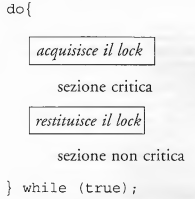
\includegraphics[scale=0.6]{img/0023.png}
\end{center}
In un sistema dotato di una singola CPU tale problema si potrebbe risolvere semplicemente se si potessero interdire le interruzioni mentre si modificano le variabili condivise. In questo modo si assicurerebbe un esecuzione ordinata e senza possibilità di prelazione della
corrente sequenza di istruzioni; non si potrebbe eseguire nessun altra istruzione, quindi non
si potrebbe apportare alcuna modifica inaspettata alle variabili condivise. questa soluzione non è sempre praticabile; la disabilitazione delle in­terruzioni nei sistemi multiprocessore può comportare sprechi di tempo dovuti alla necessi­tà di trasmettere la richiesta di disabilitazione delle interruzioni a tutte le unità d'elaborazione (diminuzione dell'efficienza).

Per questo motivo molte delle moderne architetture offrono particolari istruzioni che
permettono di controllare e modificare il contenuto di una parola di memoria, oppure di
scambiare il contenuto di due parole di memoria, in modo \textbf{atomico} - cioè come un'unità
non interrompibile.

L'istruzione \texttt{TestAndSet()} è eseguita atomicamente, cioè come un'unità non soggetta a interruzioni; quindi,
se si eseguono contemporaneamente due istruzioni \texttt{TestAndSet()}, ciascuna in un'unità
d'elaborazione diversa, queste vengono eseguite in modo sequenziale in un ordine arbitra­rio.
\begin{center}
  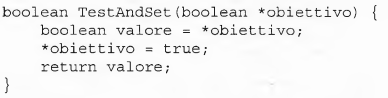
\includegraphics[scale=0.6]{img/0024.png}
\end{center}
Se si dispone dell'istruzione \texttt{TestAndSet()}, si può realizzare la mutua esclusione di­chiarando una variabile booleana globale \texttt{lock}, inizializzata a \texttt{false}.
\begin{center}
  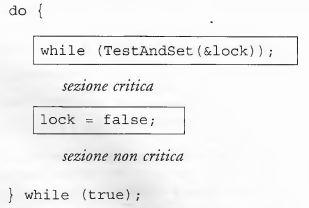
\includegraphics[scale=0.6]{img/0025.png}
\end{center}
%
L'istruzione \texttt{Swap()}, agisce sul contenuto di due parole di
memoria; anch'essa è eseguita atomicamente.
\begin{center}
  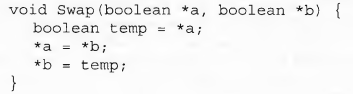
\includegraphics[scale=0.6]{img/0026.png}
\end{center}
La mutua esclusione si garantisce dichiarando e inizializzando al
valore \texttt{false} una variabile booleana globale \texttt{lock}. Inoltre, ogni processo possiede anche una
variabile booleana locale \texttt{chiave}.
\begin{center}
  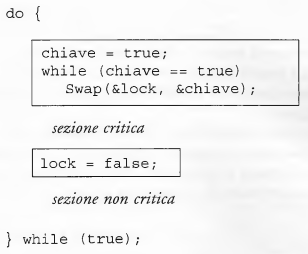
\includegraphics[scale=0.6]{img/0027.png}
\end{center}
%
Questi algoritmi soddisfano il requisito della mutua esclusione, ma non quello dell'atte­sa limitata.
Di seguito, un algoritmo che sfrutta l'istruzione \texttt{TestAndSet()}
per soddisfare tutti e tre i requisiti desiderati. Le strutture dati condivise sono:
\texttt{boolean attesa[n];}\\
\texttt{boolean lock;}\\
e sono inizializzate al valore \texttt{false}.

\subsection{Semafori}
Un \textbf{semaforo}\index{semaforo} \texttt{S} è una variabile intera cui si può accedere, escludendo l'inizializzazione,
solo tramite due operazioni atomiche predefìnite: \texttt{wait()} e \texttt{signal()}. Queste operazioni
erano originariamente chiamate rispettivamente \texttt{P} e \texttt{V}.\\
La definizione classica di \texttt{wait()} in pseudocodice
è la seguente:
\begin{center}
  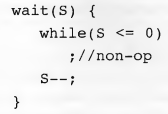
\includegraphics[scale=0.6]{img/0028.png}
\end{center}
La definizione classica di \texttt{signal()} in pseudocodice è la seguente:
\begin{center}
  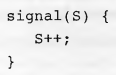
\includegraphics[scale=0.6]{img/0029.png}
\end{center}
%
Tutte le modifiche al valore del semaforo contenute nelle operazioni \texttt{wait()} e \texttt{signal()}
si devono eseguire in modo indivisibile. Inoltre, nel
caso della \texttt{wait(S)} si devono eseguire senza interruzione anche la verifica del valore intero
di \texttt{S (S $<=$ 0)} e la sua possibile modifica \texttt{(S--)}.

\subsubsection{Uso dei semafori}
Si usa distinguere tra \textbf{semafori contatore}, il cui valore numerico è illimitato, e i \textbf{semafori bi­nari}, il cuà valore è 0 o 1 . In relazione a certi sistemi i semafori binari sono anche detti \textbf{lock mutex}\index{lock mutex} (\emph{mutex locks}), perché fungono da "lock" che garantiscono la mutua esclusione.

I semafori sono utilizzabili per risolvere il problema della sezione critica con $n$ processi. Gli $n$ processi condividono un semaforo comune, \texttt{mutex}, inizializzato a 1.
\begin{center}
  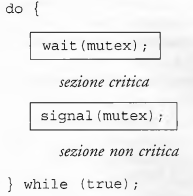
\includegraphics[scale=0.6]{img/0030.png}\\
  \caption{Realizzazione di mutua esclusione con semafori.}
\end{center}
%
I semafori sono utilizzabili anche per risolvere diversi problemi di sincronizzazione. Si
considerino, per esempio, due processi in esecuzione concorrente: $P_1$ con un'istruzione $S_1$ e
$P_2$ con un'istruzione $S_2$. Si supponga di voler eseguire $S_2$ solo dopo che $S_1$ è terminata.
Questo schema si può realizzare facendo condividere a $P_1$ e $P_2$ un semaforo comune,\texttt{sincronizzazione}, inizializzato a 0, e inserendo nel processo $P_1$ le istruzioni\medskip\\
\texttt{S$_1$\\
        signal(sincronizzazione);}\medskip\\
e nel processo $P_2$ le istruzioni\medskip\\
\texttt{wait(sincronizzazione);\\
        S$_2$;}\medskip\\
%
Poiché \texttt{sincronizzazione} è inizializzato a 0, $P_2$ esegue $S_2$ solo dopo che $P_1$ ha eseguito
\texttt{signal(sincronizzazione)}, che si trova dopo $S_1$.

\subsubsection{Realizzazione}
Il principale svantaggio della definizione di semaforo è che richiede una condizione di \textbf{atte­sa attiva} (\emph{busy waiting}). Mentre un processo si trova nella propria sezione critica, qualsiasi
altro processo che tenti di entrarvi si trova sempre nel ciclo del codice della sezione d'ingres­so. Questo tipo di semaforo è anche detto \textbf{spinlock},\index{spinlock}
perché i processi "girano" (\emph{spin}) mentre attendono al semaforo. (I semafori spinlock hanno
però il vantaggio di non richiedere cambio di contesto nel caso in cui un processo sia fermo
in attesa. Tali cambi di contesto possono essere piuttosto costosi, in termini di tempo.
(i semafori spinlock sono utili quando i lock sono applicati per brevi intervalli
di tempo)

Per superare la necessità dell'attesa attiva, si possono modificare le definizioni delle
operazioni \texttt{wait()} e \texttt{signal}: quando un processo invoca l'operazione \texttt{wait()} e trova
che il valore del semaforo non è positivo, deve attendere, ma anziché restare nell'attesa atti­va può bloccare se stesso. L'operazione di bloccaggio pone il processo in una coda d'attesa as­sociata al semaforo e cambia lo stato del processo nello stato d'attesa.

Un processo bloccato, che attende a un semaforo \texttt{S}, sarà riavviato in seguito all'esecu­zione di un'operazione \texttt{signal()} su \texttt{S} da parte di qualche altro processo. Il processo si riav­via tramite un'operazione \texttt{wait()}, che modifica lo stato del processo da attesa a pronto.
Il processo entra nella coda dei processi pronti.

L'operazione \texttt{block()} sospende il processo che la invoca; l'operazione \texttt{wakeup(P)} pone in
stato di pronto per l'esecuzione un processo \texttt{P} bloccato. Queste due operazioni sono fornite
dal sistema operativo come chiamate di sistema di base.

La lista dei processi che attendono a un semaforo si può facilmente realizzare inseren­do un campo puntatore in ciascun blocco di controllo del processo (PCB).

I semafori devono essere eseguiti in modo atomico.

\subsubsection{Stallo e attesa}
La realizzazione di un semaforo con coda d'attesa può condurre a situazioni in cui ciascun
processo di un insieme di processi attende indefinitamente un evento — l'esecuzione di
un'operazione \texttt{signal()} — che può essere causato solo da uno dei processi dello stesso in­sieme. Quando si verifica una situazione di questo tipo si dice che i processi sono \textbf{in stallo}\index{stallo}
(\emph{deadlocked}).\index{deadlock}

Un'altra questione connessa alle situazioni di stallo è quella dell'\textbf{attesa indefinita} (\emph{starvation}).\index{starvation}

\subsubsection{Inversione di priorità}
Nello scheduling dei processi si possono incontrare difficoltà ogniqualvolta un processo a
priorità più alta abbia bisogno di leggere o modificare dati a livello kernel utilizzati da un
processo, o da una catena di processi, a priorità più bassa. Visto che i dati a livello kernel so­no tipicamente protetti da un lock, il processo a priorità maggiore dovrà attendere finché il
processo a priorità minore non avrà finito di utilizzare le risorse. La situazione si complica
ulteriormente se il processo a priorità più bassa ha dovere di prelazione su un processo a
priorità più alta. Assumiamo, ad esempio, che vi siano tre processi L, M e H, le cui priorità
seguono l'ordine L < M < H. Assumiamo che il processo H richieda la risorsa R alla quale sta
accedendo il processo L. Usualmente il processo H resterebbe in attesa che L liberi la risorsa
R. Supponiamo però che M diventi eseguibile, con prelazione sul processo L. Avviene che un processo con priorità più bassa, il processo M, influenzi il tempo che H
attenderà in attesa della risorsa R.

Questo problema è noto come \textbf{inversione della priorità}. Solitamente questi sistemi risolvono il problema implementando un
\textbf{protocollo di ereditarietà delle priorità}, secondo il quale tutti i processi che stanno acce­dendo a risorse di cui hanno bisogno processi con priorità maggiore ereditano la priorità più
alta finché non finiscono di utilizzare le risorse in questione. Quando hanno terminato, la
loro priorità ritorna al valore originale.

\subsection{Problemi tipici di sincronizzazione}
\subsubsection{Produttori e consumatori con memoria limitata}
Il problema dei produttori e consumatori con memoria limitata si usa generalmente per illustrare la potenza delle primitive di sincronizzazione.

Si supponga di disporre di una certa quantità di memoria rappresentata da un buffer
con $n$ posizioni, ciascuna capace di contenere un elemento. Il semaforo \texttt{mutex} garantisce la
mutua esclusione degli accessi al buffer ed è inizializzato al valore 1. I semafori \texttt{vuote} e
\texttt{piene} conteggiano rispettivamente il numero di posizioni vuote e il numero di posizioni
piene nel buffer. Il semaforo \texttt{vuote} si inizializza al valore \texttt{n}; il semaforo \texttt{piene} si inizializza al valore 0.

\subsubsection{Problema dei lettori-scrittori}
Si supponga una base di dati da condividere tra numerosi processi concorrenti. Alcuni
processi possono richiedere solo la lettura del contenuto dell'oggetto condiviso, mentre altri
possono richiedere un aggiornamento, vale a dire una lettura e una scrittura, dello stesso og­
getto. Questi due processi sono distinti, e si indicano chiamando \textbf{lettori} quelli interessati al­
la sola lettura e \textbf{scrittori} gli altri. Se due lettori accedono nello stesso momento all'insieme di dati condiviso, non si ha alcun effetto negativo; viceversa, se uno scrit­tore e un altro processo (lettore o scrittore) accedono contemporaneamente alla stessa base
di dati, ne può derivare il caos.

Per impedire l'insorgere di difficoltà di questo tipo è necessario che gli scrittori abbia­no un accesso esclusivo alla base di dati condivisa. Questo problema di sincronizzazione è
conosciuto come \textbf{problema dei lettori-scrittori}.

Il problema dei
lettori-scrittori ha diverse varianti, che implicano tutte l'esistenza di priorità; la più sempli­ce, cui si fa riferimento come al primo problema dei lettori-scrittori, richiede che nessun let­tore attenda, a meno che uno scrittore abbia già ottenuto il permesso di usare l'insieme di
dati condiviso.

Il secondo problema dei lettori-scrittori si fonda sul presupposto che uno scrittore, una volta pronto, esegua il proprio com­pito di scrittura al più presto. In altre parole, se uno scrittore attende l'accesso all'insieme di
dati, nessun nuovo lettore deve iniziare la lettura.

La soluzione del primo problema e quella del secondo possono condurre a uno stato
d'attesa indefinita (\emph{starvation}), degli scrittori, nel primo caso; dei lettori, nel secondo. Per
questo motivo sono state proposte altre varianti.

La soluzione del primo problema dei lettori-scrittori prevede dunque la condivisione
da parte dei processi lettori delle seguenti strutture dati:\\
\texttt{semaforo mutex, scrittura;\\
        int numlettori;}\\
I semafori \texttt{mutex} e \texttt{scrittura} sono inizializzati a 1; \texttt{numlettori} è inizializzato a 0. Il
semaforo \texttt{scrittura} è comune a entrambi i tipi di processi (lettura e scrittura). Il semafo­ro \texttt{mutex} si usa per assicurare la mutua esclusione al momento dell'aggiornamento di
\texttt{numlettori}. La variabile \texttt{numlettori} contiene il numero dei processi che stanno attual­mente leggendo l'insieme di dati. Il semaforo \texttt{scrittura} funziona come semaforo di mutua esclusione per gli scrittori e serve anche al primo o all'ultimo lettore che entra o esce dal­la sezione critica.

Le soluzioni al problema dei lettori-scrittori sono state generalizzate su alcuni sistemi
in modo da fornire \textbf{lock di lettura-scrittura}. Per acquisire un tale lock, è necessario specificare la modalità di scrittura o di lettura: se il processo desidera solo leggere i dati condivisi,
richiede un lock di lettura-scrittura in modalità lettura; se invece desidera anche modificare
i dati, lo richiede in modalità scrittura. E permesso a più processi di acquisire lock di lettura-scrittura in modalità lettura, ma solo un processo alla volta può avere il lock di lettura-scrittura in modalità scrittura.

\subsubsection{Problema dei cinque filosofi}
Si considerino cinque filosofi che trascorrono la loro esistenza pensando e mangiando. I fi­losofi condividono un tavolo rotondo circondato da cinque sedie, una per ciascun filosofo.
Al centro del tavolo si trova una zuppiera colma di riso, e la tavola è apparecchiata con cinque bacchette. Quando un filosofo pensa, non interagisce con i colleghi;
quando gli viene fame, tenta di prendere le bacchette più vicine: quelle che si trovano tra lui
e i commensali alla sua destra e alla sua sinistra. Un filosofo può prendere una bacchetta al­la volta e non può prendere una bacchetta che si trova già nelle mani di un suo vicino.
Quando un filosofo affamato tiene in mano due bacchette contemporaneamente, mangia
senza lasciare le bacchette. Terminato il pasto, le posa e riprende a pensare.
Il problema dei cinque filosofi è considerato un classico problema di sincronizzazione.

Una semplice soluzione consiste nel rappresentare ogni bacchetta con un semaforo: un
filosofo tenta di afferrare ciascuna bacchetta eseguendo un'operazione \texttt{wait()} su quel semaforo e la posa eseguendo operazioni \texttt{signal()} sui semafori appropriati. Quindi, i dati
condivisi sono\medskip\\
\texttt{semaforo bacchetta[5];}\medskip\\
dove tutti gli elementi \texttt{bacchetta} sono inizializzati a 1.
\begin{center}
  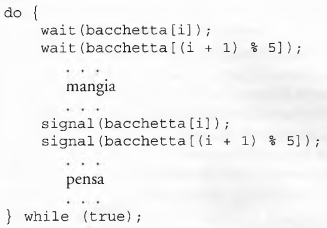
\includegraphics[scale=0.6]{img/0031.png}\\
  \caption{Struttura del filosofo i.}
\end{center}
Questa soluzione garantisce che due vicini non mangino contemporaneamente, ma è
insufficiente poiché non esclude la possibilità che si abbia una situazione di stallo. Si sup­ponga che tutti e cinque i filosofi abbiano fame contemporaneamente e che ciascuno tenti
di afferrare la bacchetta di sinistra; tutti gli elementi di \texttt{bacchetta} diventano uguali a zero, perciò ogni filosofo che tenta di afferrare la bacchetta di destra entra in stallo. Di segui­to sono elencate diverse possibili soluzioni per tali situazioni di stallo:\\
- solo quattro filosofi possono stare contemporaneamente a tavola;\\
- un filosofo può prendere le sue bacchette solo se sono entrambe disponibili (occorre
notare che quest'operazione si deve eseguire in una sezione critica);\\
- si adotta una soluzione asimmetrica: un filosofo dispari prende prima la bacchetta di
sinistra e poi quella di destra, invece un filosofo pari prende prima la bacchetta di de­stra e poi quella di sinistra.

\subsection{Monitor}
Neanche l'uso dei semafori esclude la possibilità che si verifichi qualche
errore di sincronizzazione:
\begin{itemize}[leftmargin=*]
  \item Supponiamo che un processo capovolga l'ordine in cui sono eseguite le istruzioni \texttt{wait()} e \texttt{signal()}, in questo modo:\medskip\\
  \texttt{signal(mutex);}\\
  ...\\
  sezione critica\\
  ...\\
  \texttt{wait(mutex);}\medskip\\
  In questa situazione, numerosi processi possono eseguire le proprie sezioni critiche allo stesso tempo, infrangendo il requisito della mutua esclusione. Questo errore può esse­re scoperto solo qualora diversi processi siano attivi simultaneamente nelle rispettive sezioni critiche. Si osservi che tale situazione potrebbe non essere sempre riproducibile.

  \item Ipotizziamo che un processo sostituisca \texttt{signal(mutex)} con \texttt{wait(mutex)}, cioè che esegua\medskip\\
  \texttt{wait(mutex);}\\
  ...\\
  sezione critica\\
  ...\\
  \texttt{wait(mutex);}\medskip\\
  Si genera, in questo caso, uno stallo (\emph{deadlock}).

  \item Si supponga che un processo ometta \texttt{wait(mutex)}, \texttt{signal(mutex)}, o entrambi.
  In questo caso si viola la mutua esclusione oppure si genera uno stallo.
\end{itemize}
%
Per rimediare a questi errori, i ricercatori hanno sviluppato costrutti con un linguaggio
ad alto livello, come \textbf{monitor}.

\subsubsection{Uso del costrutto monitor}
Il tipo monitor presenta un insieme di operazioni definite
dal programmatore che, all'interno del monitor, sono contraddistinte dalla mutua esclusio­ne. Il tipo monitor contiene anche la dichiarazione delle variabili i cui valori definiscono lo
stato di un'istanza del tipo, oltre ai corpi delle procedure o funzioni che operano su tali variabili.
\begin{center}
  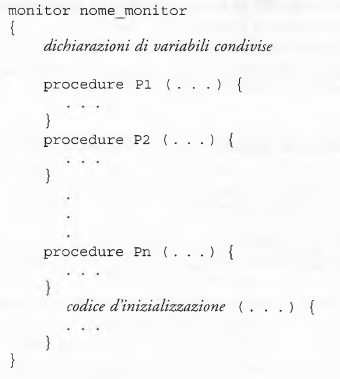
\includegraphics[scale=0.6]{img/0032.png}\\
  \caption{Sintassi di un monitor.}
\end{center}
La rappresentazione di un ti­po monitor non può essere usata direttamente dai vari processi. Pertanto, una procedura de­finita all'interno di un monitor ha accesso unicamente alle variabili dichiarate localmente,
situate nel monitor, e ai relativi parametri formali. In modo analogo, alle variabili locali di
un monitor possono accedere solo le procedure locali.

Il costrutto monitor assicura che all'interno di un monitor possa essere attivo un solo
processo alla volta, sicché non si deve codificare esplicitamente il vincolo di mutua esclusio­ne. Tale definizione di monitor non è abbastanza potente per esprimere alcu­ni schemi di sincronizzazione, sono perciò necessari ulteriori meccanismi che, in questo ca­so, sono forniti dal costrutto \texttt{condition}.

Un programmatore che deve scrivere un proprio schema di sincronizzazione può definire
una o più variabili condizionali:\medskip\\
\texttt{condition x, y;}\medskip\\
Le uniche operazioni eseguibili su una variabile \texttt{condition} sono \texttt{wait()} e \texttt{signal()}.

\subsubsection{Realizzazione di un monitor per mezzo di semafori}
A ogni monitor si associa un semaforo \texttt{mutex}, inizializzato a 1; un processo deve
eseguire \texttt{wait(mutex)} prima di entrare nel monitor, e \texttt{signal(mutex)} dopo aver lascia­to il monitor.

Poiché un processo che esegue una \texttt{signal()} deve attendere finché il processo risve­gliato si metta in attesa o lasci il monitor, si introduce un altro semaforo, \texttt{prossimo}, ini­zializzato a 0, a cui i processi che eseguono una \texttt{signal()} possono autosospendersi. Per
contare i processi sospesi al semaforo \texttt{prossimo}, si usa una variabile intera
\texttt{prossimo\_contatore}. Quindi, ogni procedura esterna di monitor \texttt{F} si sostituisce col se­guente codice:
\begin{center}
  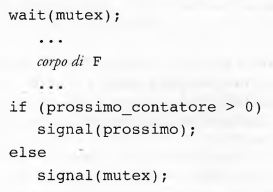
\includegraphics[scale=0.6]{img/0033.png}
\end{center}
Per ogni
variabile x di tipo \texttt{condition} si introducono un semaforo \texttt{x\_sem} e una variabile intera
\texttt{x\_contatore}, entrambi inizializzati a 0. L'operazione \texttt{x.wait()} si può realizzare come
segue:
\begin{center}
  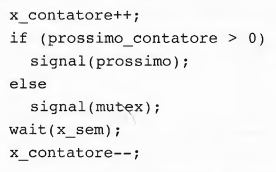
\includegraphics[scale=0.6]{img/0034.png}
\end{center}
L'operazione \texttt{x.signal} si può realizzare come segue:
\begin{center}
  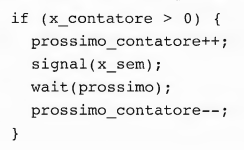
\includegraphics[scale=0.6]{img/0035.png}
\end{center}

\subsubsection{Ripresa dei processi all'interno di un monitor}
Se più processi sono sospesi alla condizione x, e se qualche processo esegue l'ope­razione \texttt{x.signal()}, è necessario stabilire quale tra i processi sospesi si debba riattivare per
primo. Una semplice soluzione consiste nell'usare un ordinamento FCFS, secondo cui il pro­cesso che attende da più tempo viene ripreso per primo. Tuttavia, in molti casi uno schema
di scheduling di questo tipo non risulta adeguato; in questi casi si può usare un costrutto di
attesa condizionale della forma\\ \texttt{x.wait(c);}\\
dove con c si indica un'espressione intera che si valuta al momento dell'esecuzione dell'ope­razione \texttt{wait()}. Il valore di c, chiamato \textbf{numero di priorità}, viene poi memorizzato col no­me del processo sospeso. Quando si esegue \texttt{x.signal()}, si riprende il processo cui è asso­ciato il numero di priorità più basso.

\subsection{Transazioni atomiche}
La mutua esclusione nelle sezioni critiche assicura che siano eseguite in modo atomico.

\subsubsection{Modello di sistema}
Un insieme di istruzioni (operazioni) che esegue una singola funzione logica prende il nome
di \textbf{transazione}.\index{transazione}

Una transazione è un'unità di programma che accede a elementi contenuti in file resi­
denti nella memoria secondaria ed eventualmente li aggiorna. È sufficiente considerare una transazione come una sequenza di operazioni \texttt{read}
e \texttt{write}, terminate da un'operazione \texttt{commit} o da \texttt{abort}. L'operazione \texttt{commit} indica
che la transazione è terminata con successo, mentre l'operazione \texttt{abort} significa che la
transazione è fallita, a causa di qualche errore logico o di un guasto del sistema.

La terminazione anomala di una transazione non deve produrre alcun effetto sullo
stato dei dati che questa ha già modificato.
Quindi, è necessario ripristinare lo stato dei dati adoperati dalla transazione fallita, ri­portandolo a quello che li caratterizzava appena prima dell'inizio della transazione (\textbf{rollback})\index{rollback}.

Per stabilire il modo in cui un sistema deve garantire l'atomicità delle proprie transa­zioni, è necessario identificare le proprietà dei dispositivi che si usano per memorizzare i da­ti ai quali esse accedono:
\begin{itemize}
  \item \textbf{Memorie volatili}. Le informazioni registrate nelle memorie volatili, per esempio la memoria centrale o le cache, di solito non sopravvivono ai crolli del sistema. L'accesso a questo tipo di dispositivi è molto rapido.
  \item \textbf{Memorie non volatili}. Le informazioni registrate in memorie non volatili, per esem­pio dischi e nastri magnetici, di solito sopravvivono ai crolli del sistema.
  \item \textbf{Memorie stabili}. Le informazioni contenute nelle memorie stabili per definizione non si perdono mai
\end{itemize}

\subsubsection{Ripristino basato sulla registrazione delle modifiche}
Un modo per assicurare l'atomicità è registrare in memorie stabili le informazioni che de­scrivono tutte le modifiche che la transazione ha apportato ai dati a cui ha avuto accesso. In
tal senso, il metodo più largamente usato è quello della registrazione con scrittura anticipa­ta (\emph{write-ahead logging}); il sistema mantiene, nella memoria stabile, una struttura dati chia­mata \textbf{log},\index{log} in cui ciascun elemento descrive una singola operazione \texttt{write} eseguita dalla
transazione ed è composto dei seguenti campi:
\begin{itemize}
  \item nome della transazione
  \item nome del dato modificato
  \item valore precedente
  \item nuovo valore
\end{itemize}
%
Mediante l'uso dei log il sistema può gestire qualsiasi malfunzionamento, purché non
sia una perdita delle informazioni contenute nella memoria non volatile. L'algoritmo di ri­pristino impiega le due seguenti procedure:
\begin{itemize}
  \item \texttt{undo($T_i$)}, per ripristinare il precedente valore di tutti i dati modificati dalla transa­zione $T_i$;
  \item \texttt{redo($T_i$)}, per assegnare il nuovo valore a tutti i dati modificati dalla transazione $T_i$.
\end{itemize}

\subsubsection{Punti di verifica}
Quando si verifica un guasto nel sistema è necessario consultare il log per determinare qua­li transazioni annullare e quali ripetere. La ricerca può richiedere un tempo piuttosto lungo.
Per ridurre questo genere di sprechi si introduce il concetto di \textbf{punto di verifica} (\emph{checkpoint}).\index{checkpoint}
Durante l'esecuzione il sistema esegue la registrazione con scrittura anticipata e registrazioni
periodiche, che costituiscono ciascun punto di verifica.

La presenza dell'elemento <\texttt{checkpoint}> consente al sistema di rendere più efficiente la
propria procedura di ripristino.

\subsubsection{Transazioni atomiche concorrenti}
\textbf{Serializzabilità}\\
Poiché le
transazioni sono atomiche, il risultato dell'esecuzione concorrente di più transazioni deve
essere equivalente a quello che si otterrebbe eseguendo le transazioni in una sequenza arbi­traria.\medskip\\
\textbf{Protocolli per la gestione dei lock}\\
Uno dei metodi che si usano per garantire la serializzabilità consiste nell'associare un lock a
ciascun dato, e richiedere che ogni transazione rispetti il \textbf{protocollo per la gestione dei lock}\index{lock}
(\emph{locking protocol}), che governa l'acquisizione e il rilascio dei lock. Si può applicare un lock a
un dato in in diversi modi:
\begin{itemize}
  \item \textbf{Condiviso}. Una transazione $T_i$ può leggere ma non scrivere nell'elemento
  \item \textbf{Esclusivo}. Una transazione $T_i$ può leggere e scrivere nell'elemento
\end{itemize}
Un protocollo che assicura la serializzabilità è il cosiddetto \textbf{protocollo per la gestione
dei lock a due fasi}, che esige che ogni transazione richieda l'esecuzione delle operazioni di
lock e di rilascio (\emph{unlock}) in due fasi distinte:
\begin{itemize}
  \item \textbf{fase di crescita}. Una transazione può ottenere nuovi lock sui dati, ma non rilasciarne alcuno in suo possesso;
  \item \textbf{fase di riduzione}. Una transazione può rilasciare lock sui dati di cui è in possesso, ma non ottenerne di nuovi.
\end{itemize}\medskip
\textbf{Protocolli basati sulla marcatura temporale}\\
Un altro metodo per determinare l'or­dine di serializzabilità consiste nella scelta anticipata di un ordinamento delle transazioni. Il
metodo più comunemente adottato consiste nell'usare uno schema con \textbf{ordinamento a
marche temporali} (\emph{timestamp ordering}).\index{timestamp ordering}

Per realizzare questo schema a ogni elemento Q si associano due valori di marche tem­porali:
\begin{itemize}
  \item \textbf{R-timestamp}(Q), che denota la maggiore tra le marche temporali di tutte le transazio­ni che hanno completato con successo un'operazione \texttt{read}(Q).
  \item \textbf{W-timestamp}(Q), che denota la maggiore tra le marche temporali di tutte le transa­zioni che hanno completato con successo un'operazione \texttt{write}(Q).
\end{itemize}

\section{Stallo dei processi}
In un ambiente con multiprogrammazione più processi possono competere per ottenere un
numero finito di risorse; se una risorsa non è correntemente disponibile, il processo richiedente passa allo stato d'attesa. Se le risorse richieste sono trattenute da altri processi, a loro
volta nello stato d'attesa, il processo potrebbe non cambiare più il suo stato. Situazioni di
questo tipo sono chiamate di \textbf{stallo}\index{stallo} (\emph{deadlock}).\index{deadlock}

\subsection{Modello del sistema}
Un sistema è composto da un numero finito di risorse da distribuire tra più processi in com­petizione. Le risorse sono suddivise in tipi differenti, ciascuno formato da un certo numero
di istanze identiche.
Se un sistema ha due unità d'elabo­razione, tale tipo di risorsa ha due istanze.

Se un processo richiede un'istanza relativa a un tipo di risorsa, l'assegnazione di qual­siasi istanza di quel tipo può soddisfare la richiesta. Se ciò non si verifica significa che le
istanze non sono identiche e le classi di risorse non sono state definite correttamente. Un si­stema può, per esempio, avere due stampanti; se a nessuno interessa sapere quale sia la stam­pante in funzione, le due stampanti si possono definire come appartenenti alla stessa classe
di risorse; se, però, una stampante si trova al nono piano e l'altra al piano terra, allora le due
stampanti si possono considerare non equivalenti, e per definire ciascuna delle due può es­sere necessario ricorrere a classi di risorse distinte.

Prima di adoperare una risorsa, un sistema deve richiederla e, dopo averla usata, deve
rilasciarla. Ordinarie condizioni di funzionamento:
\begin{itemize}
  \item \textbf{Richiesta}. Se la richiesta non si può soddisfare immediatamente il processo richiedente deve
attendere finché non possa acquisire tale risorsa.
  \item \textbf{Uso}. Il processo può operare sulla risorsa.
  \item \textbf{Rilascio}. Il processo rilascia la risorsa.
\end{itemize}
%
La richiesta e il rilascio di risorse avvengono tramite chiamate di sistema. Ne sono esempi le chiamate di sistema \texttt{request()} e \texttt{release()}, \texttt{open/} e \texttt{close()}, \texttt{allocate()} e \texttt{free()}. La richiesta e il rilascio di altre risorse si possono ese­guire per mezzo delle operazioni \texttt{wait()} e \texttt{signal()} su semafori.

Un gruppo di processi entra in stallo quando tutti i processi del gruppo attendono un
evento che può essere causato solo da un altro processo che si trova nello stato di attesa.

\subsection{Grafo di assegnazione delle risorse}
Le situazioni di stallo\index{stallo} si possono descrivere con maggior precisione avvalendosi di una rap­presentazione detta grafo\index{grafo di assegnazione delle risorse} di assegnazione delle risorse. Si tratta di un insieme di vertici V e
un insieme di archi E, con l'insieme di vertici V composto da due sottoinsiemi: $P = {P_1, P_2, ..., P_n}$ che rappresenta tutti i processi del sistema, e $R = {R_1, R_2, ..., R_m}$, che rappresenta tutti i tipi di risorsa del sistema.

Un arco diretto dal processo $P_i$ al tipo di risorsa $R_j$ si indica $P_i\rightarrow R_j$ (\textbf{arco di richiesta}), e significa che il
processo $P_i$ ha richiesto un'istanza del tipo di risorsa $R_j$, e attualmente attende tale risorsa.
Un arco diretto dal tipo di risorsa $R_j$ al processo $P_i$ si indica $R_j\rightarrow P_i$ (\textbf{arco di assegnazione}), e significa che un'istan­za del tipo di risorsa $R_j$ è assegnata al processo $P_i$.
Graficamente ogni processo $P_i$ si rappresenta con un cerchio e ogni tipo di risorsa $R_j$ si
rappresenta con un rettangolo. Giacché il tipo di risorsa $R_j$ può avere più di un'istanza, cia­scuna di loro si rappresenta con un puntino all'interno del rettangolo.
\begin{center}
  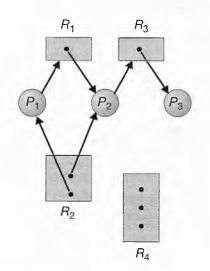
\includegraphics[scale=0.6]{img/0036.png}
\end{center}
Se il grafo
non contiene cicli, nessun processo del sistema subisce uno stallo; se il grafo contiene un ci­clo, può sopraggiungere uno stallo.
Se ciascun tipo di risorsa ha esattamente un'istanza, allora l'esistenza di un ciclo impli­ca la presenza di uno stallo; se il ciclo riguarda solo un insieme di tipi di risorsa, ciascuno dei
quali ha solo un'istanza, si è verificato uno stallo. Ogni processo che si trovi nel ciclo è in
stallo. In questo caso l'esistenza di un ciclo nel grafo è una condizione necessaria e sufficien­te per l'esistenza di uno stallo.
Se ogni tipo di risorsa ha più istanze, un ciclo non implica necessariamente uno stallo.
In questo caso l'esistenza di un ciclo nel grafo è una condizione necessaria ma non sufficien­te per l'esistenza di uno stallo.

\subsection{Evitare le situazioni di stallo}
Un metodo per evitare le situazioni di stallo consiste nel richiedere ulterio­ri informazioni sulle modalità di richiesta delle risorse.

Gli algoritmi differiscono tra loro per la quantità e il tipo di informazioni richieste. Il
modello più semplice e più utile richiede che ciascun processo dichiari il \emph{numero massimo}
delle risorse di ciascun tipo di cui necessita. Data un'informazione a priori per ogni proces­so sul massimo numero di risorse richiedibili per ciascun tipo, si può costruire un algoritmo
capace di assicurare che il sistema non entri in stallo.

Lo \emph{stato} di assegnazione
delle risorse è definito dal numero di risorse disponibili e assegnate e dalle richieste massime
dei processi.

\subsubsection{Stato sicuro}
Uno stato si dice sicuro se il sistema è in grado di assegnare risorse a ciascun processo (fino al
suo massimo). Più formalmente, un
sistema si trova in stato sicuro solo se esiste una sequenza sicura. Una sequenza di processi
$<P_1, P_2, ..., P_n>$ è una sequenza sicura per lo stato di assegnazione attuale se, per ogni $P_i$, le
richieste che $P_i$, può ancora fare si possono soddisfare impiegando le risorse attualmente di­sponibili più le risorse possedute da tutti i $P_j$ con $j<i$.
Se non esiste una sequenza di questo
tipo, lo stato del sistema si dice \emph{non sicuro}.

Uno stato sicuro non è di stallo. Viceversa, uno stato di stallo è uno stato non sicuro. Uno stato non sicu­ro \emph{potrebbe} condurre a uno stallo.
\begin{center}
  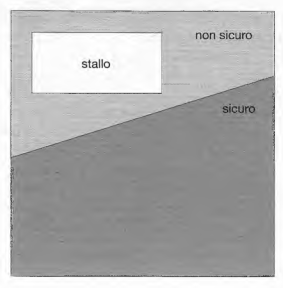
\includegraphics[scale=0.6]{img/0037.png}
\end{center}

\subsubsection{Algoritmo con grafo di assegnazione delle risorse}
Quando il sistema per l'assegnazione delle risorse è tale che ogni tipo di risorsa ha una sola
istanza, per evitare le situazioni di stallo si può far uso di una variante del grafo di assegna­zione delle risorse. Oltre agli archi di richiesta e di assegnazione,
si introduce un nuovo tipo di arco, l'\textbf{arco di reclamo} (\emph{claim edge}). Un arco di reclamo
$P_i\rightarrow R_j$ indica che il processo $P_i$ può richiedere la risorsa $R_j$ in un qualsiasi momento futu­ro. Quest'arco ha la stessa direzione dell'arco di richiesta, ma si rappresenta con una linea
tratteggiata. Quando il processo $P_i$ richiede la risorsa $R_j$ l'arco di reclamo $P_i \rightarrow R_j$ diventa un
arco di richiesta. Analogamente, quando $P_i$ rilascia la risorsa $R_j$, l'arco di assegnazione
$R_j \rightarrow P_i$ diventa un arco di reclamo $P_i \rightarrow R_j$. Occorre sottolineare che le risorse devono esse­re reclamate a priori nel sistema.

La sicurezza si controlla con un algoritmo di rilevamento dei cicli, e che un algoritmo per il rileva­mento di un ciclo in questo grafo richiede un numero di operazioni dell'ordine di $n^2$, dove
con $n$ si indica il numero dei processi del sistema.

Se non esiste alcun ciclo, l'assegnazione della risorsa lascia il sistema in uno stato sicuro. Se
invece si trova un ciclo, l'assegnazione conduce il sistema in uno stato non sicuro, e il pro­cesso $P_i$ deve attendere che si soddisfino le sue richieste.

\subsubsection{Algoritmo del banchiere}
L'algoritmo con grafo di assegnazione delle risorse non si può applicare ai sistemi di asse­
gnazione delle risorse con più istanze di ciascun tipo di risorsa. L'algoritmo per evitare le si­
tuazioni di stallo qui descritto, è noto col nome di \textbf{algoritmo del
banchiere} (l'algoritmo si potrebbe impiegare in un siste­ma bancario per assicurare che la banca non assegni mai tutto il denaro disponibile, poiché,
se ciò avvenisse, non potrebbe più soddisfare le richieste di tutti i suoi clienti).

Quando si presenta, un nuovo processo deve dichiarare il numero massimo delle istan­ze di ciascun tipo di risorsa di cui necessita. Questo numero non può superare il numero to­tale delle risorse del sistema. Quando un utente richiede un gruppo di risorse, si deve stabi­lire se l'assegnazione di queste risorse lasci il sistema in uno stato sicuro. Se si rispetta tale
condizione, si assegnano le risorse, altrimenti il processo deve attendere che qualche altro
processo ne rilasci un numero sufficiente.

La realizzazione dell'algoritmo del banchiere richiede la gestione di alcune strutture
dati che codificano lo stato di assegnazione delle risorse del sistema. Sia $n$ il numero di pro­cessi del sistema e $m$ il numero dei tipi di risorsa. Sono necessarie le seguenti strutture dati:
\begin{itemize}
  \item \textbf{Disponibili}. Un vettore di lunghezza m indica il numero delle istanze disponibili per
ciascun tipo di risorsa
  \item \textbf{Massimo}. Una matrice $n\times m$ definisce la richiesta massima di ciascun processo
  \item \textbf{Assegnate}. Una matrice $n\times m$ definisce il numero delle istanze di ciascun tipo di ri­sorsa attualmente assegnate a ogni processo
  \item \textbf{Necessità}. Una matrice $n\times m$ indica la necessità residua di risorse relativa a ogni pro­cesso
\end{itemize}

\subsubsection{Algoritmo di verifica della sicurezza}
\begin{itemize}[leftmargin=*]
  \item Siano $Lavoro$ e $Fine$ vettori di lunghezza rispettivamente $m$ e $n$.\\
  inizializza $Lavoro = Disponibili$ e $Fine[i] = falso$, per $i = 1, 2, ..., n-1$;
  \item cerca un indice $i$ tale che valgano contemporaneamente le seguenti relazioni:\\
  a) $Fine[i] == falso$\\
  b) $Necessita'_i <= Lavoro$\\
  se tale $i$ non esiste, esegue il passo 4;
  \item $Lavoro = Lavoro + Assegnate_i$\\
  $Fine[i] = vero$\\
  torna al passo 2
  \item se $Fine[i] == vero$ per ogni $i$, allora il sistema è in uno stato sicuro.
\end{itemize}
%
Per determinare se uno stato è sicuro tale algoritmo può richiedere un numero di operazio­ni dell'ordine di $m \times n^2$.

\subsubsection{Algoritmo di richiesta delle risorse}
Sia $Richieste_i$ il vettore delle richieste per il processo $P_i$. Se $Richieste_i[j]==k$, allora il
processo $P_i$ richiede $k$ istanze del tipo di risorsa $R_j$. Se il processo $P_i$ fa una richiesta di risor­se, si svolgono le seguenti azioni:
\begin{itemize}[leftmargin=*]
  \item se $Richieste_i <= Necessita'_i$, esegue il passo 2, altrimenti riporta una condizione d'errore,
  poiché il processo ha superato il numero massimo di richieste;
  \item se $Richieste_i <= Disponibili$, esegue il passo 3, altrimenti $P_i$ deve attendere poiché le ri­  sorse non sono disponibili;
  \item simula l'assegnazione al processo $P_i$ delle risorse richieste modificando come segue lo
  stato di assegnazione delle risorse:\\
  $Disponibili = Disponibili - Richieste_i$\\
  $Assegnate_i = Assegnate_i + Richieste_i$\\
  $Necessita'_i = Necessita'_i - Richieste_i$
\end{itemize}
Se lo stato di assegnazione delle risorse risultante è sicuro, la transazione è completata
e al processo $P_i$ si assegnano le risorse richieste. Tuttavia, se il nuovo stato è non sicuro,
$P_i$ deve attendere $Richieste_i$ e si ripristina il vecchio stato di assegnazione delle risorse.

\section{Memoria centrale}
\subsection{Introduzione}
La memoria è fondamentale nelle operazioni di un moderno sistema di calcolo; consiste in un ampio vettore di parole o byte, ciascuno con il pro­prio indirizzo.

Un tipico ciclo d'esecuzione di un'istruzione prevede che l'istruzione sia
prelevata dalla memoria; decodificata ed eseguita sugli eventuali operandi; i risultati si possono salvare in memoria. La
memoria vede soltanto un flusso d'indirizzi di memoria, e non sa come sono generati. È dunque possibile ignorare \emph{come}
un programma genera un indirizzo di memoria.

\subsubsection{Dispositivi essenziali}
La memoria centrale e i registri incorporati nel processore sono le sole aree di memorizza­zione a cui la CPU può accedere direttamente.
I dati che non sono in
memoria devono essere caricati prima che la CPU possa operare su di loro.

I registri incorporati nella CPU sono accessibili nell'arco di un ciclo dell'orolo­gio di sistema. Molte CPU sono capaci di decodificare istruzioni ed effettuare semplici opera­zioni sui contenuti dei registri alla velocità di una o più operazioni per ciclo. Ciò non vale per
la memoria centrale, cui si accede attraverso una transazione sul bus della memoria. Nei casi in
cui l'accesso alla memoria richieda molti cicli d'orologio, il processore entra necessariamente in
\textbf{stallo}\index{stallo} (\emph{stall}), poiché manca dei dati richiesti per completare l'istruzione che sta eseguendo.
Questa situazione è intollerabile. Il rimedio
consiste nell'interposizione di una memoria veloce tra CPU e memoria centrale. Un buffer di
memoria, detto cache, è in grado di conciliare le differenti velocità.

Bisogna assicurarsi che ciascun processo abbia uno spazio di memoria se­parato. A tal fine, occorre poter determinare l'intervallo degli indirizzi a cui un processo può
accedere legalmente, e garantire che possa accedere soltanto a questi indirizzi. Si può imple­mentare il meccanismo di protezione tramite due registri, detti \index{registri}\textbf{registri base} e \textbf{registri limite}.
Il registro base contiene il più piccolo indirizzo legale
della memoria fisica; il registro limite determina la dimensione deirintervallo ammesso. Ad
esempio, se i registri base e limite contengono rispettivamente i valori 300040 e 120900, al
programma si consente l'accesso alle locazioni di memoria di indirizzi compresi tra 300040
e 420939, estremi inclusi.

Per mettere in atto il meccanismo di protezione, la CPU confronta \emph{ciascun} indirizzo ge­nerato in modalità utente con i valori contenuti nei due registri. Qualsiasi tentativo da par­te di un programma eseguito in modalità utente di accedere alle aree di memoria riservate al
sistema operativo o a una qualsiasi area di memoria riservata ad altri utenti comporta l'invio
di un segnale di eccezione che restituisce il controllo al sistema operativo che, a sua volta, in­terpreta l'evento come un errore fatale.

Solo il sistema operativo può caricare i registri base e limite, grazie a una speciale istru­zione privilegiata.

\subsubsection{Associazione degli indirizzi}
In genere un programma risiede in un disco in forma di un file binario eseguibile. Per essere
eseguito, il programma va caricato in memoria e inserito all'interno di un processo. Secondo il
tipo di gestione della memoria adoperato, durante la sua esecuzione, il processo si può trasfe­rire dalla memoria al disco e viceversa. L'insieme dei processi presenti nei dischi e che attendo­no d'essere trasferiti in memoria per essere eseguiti forma la \textbf{coda d'ingresso} (\emph{input queue}).

La procedura normale consiste nello scegliere uno dei processi appartenenti alla coda
d'ingresso e nel caricarlo in memoria. Il processo durante l'esecuzione può accedere alle
istruzioni e ai dati in memoria. Quando il processo termina, si dichiara disponibile il suo
spazio di memoria.

Generalmente gli indirizzi del programma sorgente sono simboli­ci (per esempio, contatore). Un compilatore di solito \textbf{associa} (\emph{bind}) questi indirizzi simboli­ci a indirizzi rilocabili (per esempio, "14 byte dall'inizio di questo modulo"). L'editor dei
collegamenti (\emph{linkage editor}), o il caricatore (\emph{loader}),\index{loader} fa corrispondere a sua volta questi indi­rizzi rilocabili a indirizzi assoluti.
L'associazione di istruzioni e dati a indirizzi di memoria si può compie­re in qualsiasi fase del seguente percorso:
\begin{itemize}
  \item \textbf{Compilazione}. Se nella fase di compilazione si sa dove il processo risiederà in memo­ria, si può generare codice assoluto.
  \item \textbf{Caricamento}. Se nella fase di compilazione non è possibile sapere in che punto della me­moria risiederà il processo, il compilatore deve generare codice rilocabile.
  \item \textbf{Esecuzione}. Se durante l'esecuzione il processo può essere spostato da un segmento di memoria a un altro, si deve ritardare l'associazione degli indirizzi fino alla fase d'esecu­zione
\end{itemize}

\subsubsection{Spazi di indirizzi logici e fisici a confronto}
Un indirizzo generato dalla CPU di solito si indica come \textbf{indirizzo logico}, mentre un indi­rizzo visto dall'unità di memoria, cioè caricato nel \textbf{registro dell'indirizzo di memoria}
(\emph{memory address register}, MAR)\index{memory address register} di solito si indica come \emph{indirizzo fisico}.\index{indirizo fisico}

I metodi di associazione degli indirizzi nelle fasi di compilazione e di caricamento pro­ducono indirizzi logici e fisici identici. Con i metodi di associazione nella fase d'esecuzione,
invece, gli indirizzi logici non coincidono con gli indirizzi fisici. In questo caso ci si riferisce agli indirizzi logici col termine indirizzi virtuali; in questo testo si usano tali ter­mini in modo intercambiabile. L'insieme di tutti gli indirizzi logici generati da un program­ma è lo spazio degli indirizzi logici; l'insieme degli indirizzi fisici corrispondenti a tali indi­rizzi logici è lo spazio degli indirizzi fisici.

L'associazione nella fase d'esecuzione dagli indirizzi virtuali agli indirizzi fisici è svolta
da un dispositivo detto unità di gestione della memoria (\emph{memory-management unit}, MMU). Si può scegliere tra diversi metodi di realizzazio­ne di tale associazione.

Il registro di base è ora denominato \textbf{registro di rilocazione}:
quando un processo utente genera un indirizzo, prima dell'invio all'unità di memoria, si
somma a tale indirizzo il valore contenuto nel registro di rilocazione.

Il programma utente non considera mai gli indirizzi fisici \emph{reali}. Il programma crea un
puntatore alla locazione 346, lo memorizza, lo modifica, lo confronta con altri indirizzi, tut­to ciò semplicemente come un numero. Solo quando assume il ruolo di un indirizzo di me­moria (magari in una load o una store indiretta), si riloca il numero sulla base del contenu­to del registro di rilocazione. Il programma utente tratta indirizzi logici, l'architettura del si­
stema converte gli indirizzi logici in indirizzi \emph{fisici}.

La locazione finale di un riferimento a un indirizzo di memoria
non è determinata finché non si compie effettivamente il riferimento.
In questo caso esistono due diversi tipi di indirizzi: gli indirizzi logici (da 0 a max) e gli indirizzi fisici (da $r+0$ a $r+max$ per un valore di base $r$).
L'utente genera solo indirizzi logici e pensa che il processo sia eseguito nelle posizioni da $0$ a
$max$. Il programma utente fornisce indirizzi logici che, prima d'essere usati, si devono far
corrispondere a indirizzi fisici.

\subsubsection{Caricamento dinamico}
Per migliorare l'utilizzo della memoria si può ricorrere al \textbf{caricamento dinamico} (\emph{dynamic
loading}), mediante il quale si carica una procedura solo quando viene richiamata.
Si ca­rica il programma principale in memoria e quando, durante l'esecuzione, una procedura de­ve richiamarne un'altra, si controlla innanzitutto che sia stata caricata, altrimenti si richiama
il caricatore di collegamento rilocabile per caricare in memoria la procedura richiesta e aggiornare le tabelle degli indirizzi del programma in modo che registrino questo cambiamento. A questo punto il controllo passa alla procedura appena caricata.

Il vantaggio dato dal caricamento dinamico consiste nel fatto che una procedura che
non si adopera non viene caricata.

\subsubsection{Collegamento dinamico e librerie condivise}
Alcuni sistemi operativi
consentono solo il \textbf{collegamento statico}. Il concetto di collegamento dinamico è analogo a quello di caricamento
dinamico. Invece di differire il caricamento di una procedura fino al momento dell'esecu­zione, si differisce il collegamento.

Con il collegamento dinamico per ogni riferimento a una procedura di libre­ria s'inserisce all'interno dell'immagine eseguibile una piccola porzione di codice di riferi­mento (\emph{stub}), che indica come localizzare la giusta procedura di libreria residente in memo­ria o come caricare la libreria se la procedura non è già presente. Il co­dice di riferimento controlla se la procedura richiesta è già in memoria, altrimenti provvede
a caricarla; in ogni caso tale codice sostituisce se stesso con l'indirizzo della procedura, che
viene poi eseguita.

Questa caratteristica si può estendere anche agli aggiornamenti delle librerie, per
esempio, la correzione di errori. Una libreria si può sostituire con una nuova versione, e tut­ti i programmi che fanno riferimento a quella libreria usano automaticamente quella.

Questo sistema è noto anche con il nome di \textbf{librerie condivise}.

A differenza del caricamento dinamico, il collegamento dinamico richiede general­mente l'assistenza del sistema operativo.

\subsection{Avvicendamento dei processi (swapping)}
Per essere eseguito, un processo deve trovarsi in memoria centrale, ma si può trasferire tem­poraneamente in \textbf{memoria ausiliaria} (\emph{backing store}) da cui si riporta in memoria centrale al
momento di riprenderne l'esecuzione. Si consideri un ambiente di multipro­grammazione con un algoritmo circolare (\emph{round-robin}) per lo scheduling della CPU. Tra­
scorso un quanto di tempo, il gestore di memoria scarica dalla memoria il processo appena
terminato e carica un altro processo nello spazio di memoria appena liberato; questo procedimento si chiama \textbf{avvicendamento dei processi in memoria}, o \textbf{avvicendamento} o \textbf{scambio} (\emph{swapping}).\index{swapping} L'avvicendamento dei processi richiede una memoria ausiliaria per contenere tutti i processi utenti e deve permettere un accesso diretto a dette immagini di memoria. Il
sistema mantiene una \textbf{coda dei processi pronti} (\emph{ready queue}) formata da tutti i processi
pronti per l'esecuzione, le cui immagini di memoria si trovano in memoria ausiliaria o in
memoria.

\subsection{Allocazione contigua della memoria}
\subsubsection{Rilocazione e protezione della memoria}
La protezione della memoria si può realizzare usando un
registro di rilocazione con un registro limite. Il registro di rilocazione contiene il valore dell'indirizzo fisico
minore; il registro limite contiene l'intervallo di indirizzi logici. Con i registri di rilocazione e limite, ogni indirizzo logico deve
essere minore del contenuto del registro limite; la MMU fa corrispondere dinamicamente
l'indirizzo fisico all'indirizzo logico sommando a quest'ultimo il valore contenuto nel regi­stro di rilocazione.

\subsubsection{Allocazione della memoria}
Uno dei metodi più semplici per l'allocazione della memoria consiste nel suddividere la stes­sa in partizioni di dimensione fissa. Ogni partizione deve contenere esattamente un proces­so, quindi il grado di multiprogrammazione è limitato dal numero di partizioni. Con il me­todo delle partizioni multiple quando una partizione è libera può essere occupata da un processo presente nella coda d'ingresso.

Nello schema a partizione fissa il sistema operativo conserva una tabella in cui sono in­
dicate le partizioni di memoria disponibili e quelle occupate. Inizialmente tutta la memoria
è a disposizione dei processi utenti; si tratta di un grande blocco di memoria disponibile, un
\textbf{buco} (\emph{hole}).

Quando a un processo si assegna dello spazio, il processo stesso viene caricato in me­moria e può quindi competere per il controllo della CPU. Al termine, rilascia la memoria che
gli era stata assegnata, e il sistema operativo può impiegarla per un altro processo presente
nella coda d'ingresso.

In ogni dato istante è sempre disponibile una lista delle dimensioni dei blocchi liberi e
della coda d'ingresso.

In generale, è sempre presente un insieme di buchi di diverse dimensioni sparsi per la
memoria. Quando si presenta un processo che necessita di memoria, il sistema cerca nel
gruppo un buco di dimensioni sufficienti per contenerlo. Se è troppo grande, il buco viene
diviso in due parti: si assegna una parte al processo in arrivo e si riporta l'altra nell'insieme
dei buchi. Quando termina, un processo rilascia il blocco di memoria, che si reinserisce nel­
l'insieme dei buchi; se si trova accanto ad altri buchi, si uniscono tutti i buchi adiacenti per
formarne uno più grande.

Questa procedura è una particolare istanza del più generale problema di \textbf{allocazione
dinamica della memoria}, che consiste nel soddisfare una richiesta di dimensione $n$ data una
lista di buchi liberi.

Criteri:
\begin{itemize}
  \item \textbf{First-fit}. Si assegna il primo buco abbastanza grande. La ricerca può cominciare sia dal­l'inizio dell'insieme di buchi sia dal punto in cui era terminata la ricerca precedente. Si può fermare la ricerca non appena s'individua un buco libero di dimensioni sufficien­temente grandi.
  \item \textbf{Best-fit}. Si assegna il più piccolo buco in grado di contenere il processo. Ta­le criterio produce le parti di buco inutilizzate più piccole.
  \item \textbf{Worst-fit}. Si assegna il buco più grande. ale criterio produce le parti di buco inutilizzate più grandi, che possono essere più utili delle parti più piccole otte­nute col criterio precedente.
\end{itemize}

\subsubsection{Frammentazione}
Entrambi i criteri first-fit e best-fit di allocazione della memoria soffrono di frammentazio­ne esterna: quando si caricano e si rimuovono i processi dalla memoria, si frammenta lo
spazio libero della memoria in tante piccole parti. Si ha la frammentazione esterna se lo spa­zio di memoria totale è sufficiente per soddisfare una richiesta, ma non è contiguo; la me­moria è frammentata in tanti piccoli buchi. Questo problema di frammentazione può esse­re molto grave; nel caso peggiore può verificarsi un blocco di memoria libera, sprecata, tra ogni coppia di processi.

La sua gravità dipende dalla quantità totale di memoria e dalla dimensione media dei
processi. Per $n$ blocchi assegnati, si perdono altri $0,5n$ blocchi a causa della frammentazione.
Questa caratteristica è nota con il nome di \textbf{regola del 50 per cento}.

La frammentazione interna si verifica quando la memoria è suddivisa in blocchi di dimensioni fisse. Ogni volta che una richiesta di processo per la memoria, il blocco di dimensioni fisse viene assegnato al processo. Nel caso in cui la memoria assegnata al processo sia leggermente più grande della memoria richiesta, la differenza tra la memoria assegnata e richiesta è la frammentazione interna.

Questo spazio rimanente all'interno del blocco di dimensioni fisse non può essere allocato a nessun processo in quanto non sarebbe sufficiente per soddisfare la richiesta di memoria da parte del processo. Cerchiamo di capire la frammentazione interna con l'aiuto di un esempio. Lo spazio di memoria è suddiviso in blocchi di dimensioni fisse di 18.464 byte. Diciamo che una richiesta di processo per 18.460 byte e un blocco partizionato a dimensione fissa di 18.464 byte è assegnato al processo. Il risultato è 4 byte di 18.464 byte rimasti vuoti, che è la frammentazione interna.

Una soluzione al problema della frammentazione esterna è data dalla \textbf{compattazione}\index{compattazione}.
Lo scopo è quello di riordinare il contenuto della memoria per riunire la memoria libera in
un unico grosso blocco. La compattazione tuttavia non è sempre possibile: non si può rea­lizzare se la rilocazione è statica ed è fatta nella fase di assemblaggio o di caricamento; è pos­sibile solo se la rilocazione è dinamica e si compie nella fase d'esecuzione. Può essere assai oneroso.

Un'altra possibile soluzione del problema della frammentazione esterna è data dal con­sentire la non contiguità dello spazio degli indirizzi logici di un processo, permettendo così
di assegnare la memoria fisica ai processi dovunque essa sia disponibile.

\subsection{Paginazione}
La paginazione\index{paginazione} è un metodo di gestione della memoria che permette che lo spazio degli in­dirizzi fisici di un processo non sia contiguo. Elimina il gravoso problema della sistemazio­ne di blocchi di memoria di diverse dimensioni in memoria ausiliaria.

Il problema insor­ge perché, quando alcuni frammenti di codice o dati residenti in memoria centrale devono
essere scaricati, si deve trovare lo spazio necessario in memoria ausiliaria. I problemi di fram­mentazione relativi alla memoria centrale valgono anche per la memoria ausiliaria, con la
differenza che in questo caso l'accesso è molto più lento, quindi è impossibile eseguire la
compattazione.

\subsubsection{Metodo di base}
Il metodo di base per implementare la paginazione consiste nel suddividere la memoria fisi­ca in blocchi di dimensione costante, detti anche \textbf{frame}\index{frame} o \textbf{pagine fisiche}\index{pagine fisiche}, e nel suddividere
la memoria logica in blocchi di pari dimensione, detti \textbf{pagine}. Quando si deve eseguire un
processo, si caricano le sue pagine nei frame disponibili, prendendole dalla memoria ausilia­ria, divisa in blocchi di dimensione fissa, uguale a quella dei frame della memoria.

ogni indirizzo ge­nerato dalla CPU è diviso in due parti: un \textbf{numero di pagina} ($p$), e uno \textbf{scostamento} (\emph{offset})
\textbf{di pagina} (\emph{d}). Il numero di pagina serve come indice per la \textbf{tabella delle pagine}, contenen­te l'indirizzo di base in memoria fisica di ogni pagina. Questo indirizzo di base si combina con lo scostamento di pagina per definire l'indirizzo della memoria fisica.

La dimensione di una pagina, così come quella di un frame, è definita dall'architettura del
calcolatore. Se la dimensione
dello spazio degli indirizzi logici è $2^m$ e la dimensione di una pagina è di $2^n$ unità di indirizzamento (byte o parole), allora gli $m - n$ bit più significativi di un indirizzo logico indicano
il numero di pagina, e gli $n$ bit meno significativi indicano lo scostamento di pagina. L'indi­rizzo logico ha quindi la forma seguente:
\begin{center}
  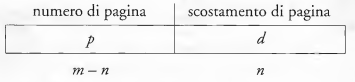
\includegraphics[scale=0.6]{img/0038.png}
\end{center}
dove $p$ è un indice della tabella delle pagine e $d$ è lo scostamento all'interno della pagina in­dicata da $p$.

La paginazione non è altro che una forma di rilocazione
dinamica: a ogni indirizzo logico l'architettura di paginazione fa corrispondere un indirizzo
fisico. L'uso della tabella delle pagine è simile all'uso di una tabella di registri base.

Con la paginazione si può evitare la frammentazione esterna: qualsiasi frame libero si
può assegnare a un processo che ne abbia bisogno; tuttavia si può avere la frammentazione
interna. I frame si assegnano come unità. L'ultimo frame assegnato
può non essere completamente pieno. Il caso peggiore si ha con un
processo che necessita di n pagine più un byte: si assegnano $n + 1$ frame, quindi si ha una
frammentazione interna di quasi un intero frame.

Conviene usare pagine di piccole dimensioni; tuttavia, a ogni elemen­to della tabella delle pagine è associato un carico che si può ridurre aumentando le dimen­sioni delle pagine. Inoltre, con un maggior numero di dati da trasferire, l'I/O su disco è più
efficiente.

Quando si deve eseguire un processo, si esamina la sua dimensione espressa in pagine.
Poiché ogni pagina del processo necessita di un frame, se il processo richiede $n$ pagine, de­vono essere disponibili almeno $n$ frame che, se ci sono, si assegnano al processo stesso. Si ca­rica la prima pagina del processo in uno dei frame assegnati e si inserisce il numero del frame
nella tabella delle pagine relativa al processo in questione. La pagina successiva si carica in
un altro frame e, anche in questo caso, si inserisce il numero del frame nella tabella delle pa­gine, e così via.

Un aspetto importante della paginazione è la netta distinzione tra la memoria vista dal­l'utente e l'effettiva memoria fìsica: il programma utente vede la memoria come un unico
spazio contiguo, contenente solo il programma stesso; in realtà, il programma utente è sparso in una memoria fisica contenente anche altri programmi. La differenza tra la memoria vi­sta dall'utente e la memoria fisica è colmata dall'architettura di traduzione degli indirizzi, che
fa corrispondere gli indirizzi fisici agli indirizzi logici generati dai processi utenti.

Poiché il sistema operativo gestisce la memoria fisica, deve essere informato dei relati­
vi particolari di allocazione: quali frame sono assegnati, quali sono disponibili, il loro nu­
mero totale, e così via. In genere queste informazioni sono contenute in una struttura dati
chiamata \textbf{tabella dei frame}.\index{tabella dei frame}

La paginazione fa aumentare la durata dei cambi di contesto.

\subsubsection{Architetture di paginazione}
L'architettura d'ausilio alla tabella delle pagine si può realizzare in modi diversi. Nel
caso più semplice, si usa uno specifico insieme di registri. Questi registri devono essere costruiti in modo da ope­rare a una velocità molto elevata.

L'uso di registri per la tabella delle pagine è efficiente se la tabella stessa è ragionevol­mente piccola, nell'ordine, per esempio, di 256 elementi. La maggior parte dei calcolatori
contemporanei usa comunque tabelle molto grandi, per esempio di un milione di elementi,
quindi non si possono impiegare i registri veloci per realizzare la tabella delle pagine; que­st'ultima si mantiene in memoria principale e un \textbf{registro di base della tabella delle pagine}
(\emph{page-table base register}, PTBR)\index{PTBR} punta alla tabella stessa. Il cambio delle tabelle delle pagine ri­chiede soltanto di modificare questo registro, riducendo considerevolmente il tempo dei
cambi di contesto.

Questo metodo presenta un problema connesso al tempo necessario di accesso a una
locazione della memoria utente.

Con questo metodo, per accedere a un byte occorro­no due accessi alla memoria (uno per l'elemento della tabella delle pagine e uno per il byte
stesso), quindi l'accesso alla memoria è rallentato di un fattore 2. Nella maggior parte dei ca­si un tale ritardo è intollerabile; sarebbe più conveniente ricorrere all'avvicendamento dei
processi!

La soluzione tipica a questo problema consiste nell'impiego di una speciale, piccola ca­che di ricerca veloce, detta TLB\index{TLB} (\emph{translation look-aside buffer}). La TLB è una memoria asso­ciativa ad alta velocità in cui ogni suo elemento consiste di due parti: una chiave, o un indi­catore (\emph{tag}) e un valore. Quando si presenta un elemento, la memoria associativa lo confronta contemporaneamente con tutte le chiavi; se trova una corrispondenza, riporta il
valore correlato. La ricerca è molto rapida, ma le memorie associative sono molto costose.

La TLB si usa insieme con le tabelle delle pagine nel modo seguente: la TLB contiene
una piccola parte degli elementi della tabella delle pagine; quando la CPU genera un indiriz­zo logico, si presenta il suo numero di pagina alla TLB; se tale numero è presente, il corrispondente numero del frame è immediatamente disponibile e si usa per accedere alla me­moria. Tutta l'operazione può richiedere un tempo inferiore al 10 per cento in più di quanto sarebbe richiesto per un riferimento alla memoria senza paginazione.

Se nella TLB non è presente il numero di pagina, situazione nota come \textbf{insuccesso della TLB}
(\emph{TLB miss}), si deve consultare la tabella delle pagine in memoria. Il numero del frame così ot­tenuto si può eventualmente usare per accedere alla memoria. Inoltre, inse
rendo i numeri della pagina e del frame nella TLB, al riferimento successivo la ricerca sarà
molto più rapida. Se la TLB è già piena d'elementi, il sistema operativo deve sceglierne uno
per sostituirlo. I criteri di sostituzione variano dalla scelta dell'elemento usato meno recen­temente (LRU) alla scelta casuale. Inoltre alcune TLB consentono che certi elementi siano
vincolati (wired down), cioè non si possano rimuovere dalla TLB; in genere si vincolano gli
elementi per il codice del kernel.

Alcune TLB memorizzano gli identificatori dello spazio d'indirizzi (\emph{address-space
identifier}, ASID) in ciascun elemento della TLB. Un ASID identifica in modo univoco ciascun
processo e si usa per fornire al processo corrispondente la protezione del suo spazio d'indiriz­zi. Quando tenta di trovare i valori corrispondenti ai numeri delle pagine virtuali, la TLB as­sicura che l'ASID per il processo attualmente in esecuzione corrisponda all'ASID associato alla
pagina virtuale. La mancata corrispondenza dell'ASID viene trattata come un insuccesso della
TLB. Inoltre, per fornire la protezione dello spazio d'indirizzi, l'ASID consente che la TLB contenga nello stesso istante elementi di diversi processi. Se la TLB non permette l'uso di ASID di­stinti, ogni volta che si seleziona una nuova tabella delle pagine, per esempio a ogni cambio
di contesto, si deve \textbf{cancellare} (\emph{flush})\index{flush} la TLB, in modo da assicurare che il successivo processo
in esecuzione non faccia uso di errate informazioni di traduzione.

La percentuale di volte che un numero di pagina si trova nella TLB è detta \textbf{tasso di suc­cessi} (\emph{hit ratio}). Un tasso di successi dell'80 per cento significa che il numero di pagina desi­derato si trova nella TLB nell'80 per cento dei casi. Se la ricerca nella TLB richiede 20 nano­secondi e sono necessari 100 nanosecondi per accedere alla memoria, allora, supponendo
che il numero di pagina si trovi nella TLB, un accesso alla memoria richiede 120 nanosecon­di. Se, invece, il numero non è contenuto nella TLB (20 nanosecondi), occorre accedere alla
memoria per arrivare alla tabella delle pagine e al numero del frame (100 nanosecondi),
quindi accedere al byte desiderato in memoria (100 nanosecondi); in totale sono necessari
220 nanosecondi. Per calcolare il \textbf{tempo effettivo d'accesso alla memoria} occorre tener con­to della probabilità dei due casi:\medskip\\
\emph{tempo effettivo d'accesso} $= 0.80\times120+0,20\times220=140$ nanosecondi\medskip\\
In questo esempio si verifica un rallentamento del 40 per cento nel tempo d'accesso alla me­moria (da 100 a 140 nanosecondi).
Per un tasso di successi del 98 per cento si ottiene il seguente risultato:\medskip\\
\emph{tempo effettivo d'accesso} $= 0.98\times120+0,02\times220=122$ nanosecondi\medskip\\
Aumentando il tasso di successi, il rallentamento del tempo d'accesso alla memoria scende
al 22\%.

\subsubsection{Protezione}
In un ambiente paginato, la protezione della memoria è assicurata dai bit di protezione as­sociati a ogni frame; normalmente tali bit si trovano nella tabella delle pagine.
Un bit può determinare se una pagina si può leggere e scrivere oppure soltanto legge­re. Tutti i riferimenti alla memoria passano attraverso la tabella delle pagine per trovare il
numero correto del frame; quindi mentre si calcola l'indirizzo fisico, si possono controllare
i bit di protezione per verificare che non si scriva in una pagina di sola lettura.

Di solito si associa a ciascun elemento della tabella delle pagine un ulteriore bit, detto
\textbf{bit di validità}. Tale bit, impostato a \emph{valido}, indica che la pagina corrispondente è nello spa­zio d'indirizzi logici del processo, quindi è una pagina valida; impostato a \emph{non valido}, indicache la pagina non è nello spazio d'indirizzi logici del processo.

Alcune architetture dispongono di registri, detti
\textbf{registri di lunghezza della tabella delle pagine} (\emph{page-table length register}, PTLR)\index{PTLR}, per indica­re le dimensioni della tabella. Questo valore si controlla rispetto a ogni indirizzo logico per
verificare che quest'ultimo si trovi nell'intervallo valido per il processo.

\subsubsection{Pagine condivise}
Un altro vantaggio della paginazione consiste nella possibilità di \emph{condividere} codice comune. Si
consideri un sistema con 40 utenti, ciascuno dei quali usa un elaboratore di testi. Se tale
programma è formato da 150 KB di codice e 50 KB di spazio di dati, per gestire i 40 utenti sono necessari 8000 KB. Se però il codice è rientrante, può essere condiviso.

Il \textbf{codice rientrante}, detto anche \textbf{codice puro}, è un codice non automodifìcante: non
cambia durante l'esecuzione. Quindi, due o più processi possono eseguire lo stesso codice
nello stesso momento. Ciascun processo dispone di una propria copia dei registri e di una
memoria dove conserva i dati necessari alla propria esecuzione. I dati per due differenti pro­cessi variano, ovviamente, per ciascun processo.

In memoria fisica è presente una sola copia dell'elaboratore di testi: la tabella delle pa­gine di ogni utente fa corrispondere gli stessi frame contenenti l'elaboratore di testi, mentre
le pagine dei dati si fanno corrispondere a frame diversi. Quindi per gestire 40 utenti sono
sufficienti una copia dell'elaboratore di testi (150 KB) e 40 copie dei 50 KB di spazio di dati
per ciascun utente; per un totale di 2150 KB, invece di 8000 KB.
Si possono condividere anche altri programmi d'uso frequente: compilatori, interfacce
a finestre, sistemi di basi di dati e così via.

\subsection{Struttura della tabella delle pagine}
\subsubsection{Paginazione gerarchica}
La maggior parte dei moderni calcolatori dispone di uno spazio d'indirizzi logici molto
grande (da 232 a 264 elementi). In un ambiente di questo tipo la stessa tabella delle pagine fi­nirebbe per diventare eccessivamente grande.

Chiaramente, sarebbe meglio evitare di col­locare la tabella delle pagine in modo contiguo in memoria centrale. Una semplice soluzio­ne a questo problema consiste nel suddividere la tabella delle pagine in parti più piccole.

Un metodo consiste nell'adottare un algoritmo di paginazione a due livelli, in cui la
tabella stessa è paginata. Si consideri il precedente esempio di macchina a 32
bit con dimensione delle pagine di 4 KB. Si suddivide ciascun indirizzo logico in un nume­ro di pagina di 20 bit e in uno scostamento di pagina di 12 bit. Paginando la tabella delle pagine, anche il numero di pagina è a sua volta suddiviso in un numero di pagina di 10 bit
e uno scostamento di pagina di 10 bit. Quindi, l'indirizzo logico è:
\begin{center}
  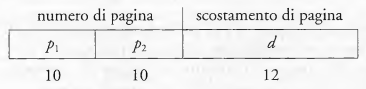
\includegraphics[scale=0.6]{img/0039.png}
\end{center}
dove $p_1$ è un indice della tabella delle pagine di primo livello, o tabella esterna delle pagine,
e $p_2$ è lo scostamento all'interno della pagina indicata dalla tabella esterna delle pagine.

Questo metodo è anche noto come \textbf{tabella delle pagine ad associazione diretta}
(\emph{forward-mapped page table}).

\subsubsection{Tabella delle pagine di tipo hash}
Un metodo di gestione molto comune degli spazi d'indirizzi relativi ad architetture oltre i
32 bit consiste nell'impiego di una \textbf{tabella delle pagine di tipo hash}, in cui l'argomento del­la funzione hash è il numero della pagina virtuale. Per la gestione delle collisioni, ogni ele­mento della tabella hash contiene una lista concatenata di elementi che la funzione hash facorrispondere alla stessa locazione. Ciascun elemento è composto da tre campi: (1) il numero della pagina virtuale; (2) l'indirizzo del frame (pagina fisica) corrispondente alla pagina
virtuale; (3) un puntatore al successivo elemento della lista.

Si applica la funzione hash al numero della pagina vir­tuale contenuto nell'indirizzo virtuale, identificando un elemento della tabella. Si confronta
il numero di pagina virtuale con il campo (1) del primo elemento della lista concatenata
corrispondente. Se i valori coincidono, si usa l'indirizzo del relativo frame (campo 2) per ge­nerare l'indirizzo fisico desiderato. Altrimenti, l'algoritmo esamina allo stesso modo gli ele­menti successivi della lista concatenata. Le tabelle delle pagine di tipo hash so­no particolarmente utili per gli spazi d'indirizzi sparsi, in cui i riferimenti alla memoria non
sono contigui ma distribuiti per tutto lo spazio d'indirizzi.

Per questo schema è stata proposta una variante, adatta a spazi di indirizzamento a 64
bit. Si tratta della \textbf{tabella delle pagine a gruppi} (\emph{clusteredpage table}), simile alla tabella hash;
ciascun elemento della tabella delle pagine contiene però i riferimenti alle pagine fisiche cor­rispondenti a un gruppo di pagine virtuali contigue. In questo modo si ri­duce lo spazio di memoria richiesto.

\subsubsection{Tabella delle pagine invertita}
Generalmente, si associa una tabella delle pagine a ogni processo e tale tabella contiene un
elemento per ogni pagina virtuale che il processo sta utilizzando, oppure un elemento per
ogni indirizzo virtuale a prescindere dalla validità di quest'ultimo. Questa è una rappresen­tazione naturale della tabella. Poiché la tabella è ordinata per indirizzi virtuali, il sistema operativo può
calcolare in che punto della tabella si trova l'elemento dell'indirizzo fisico associato, e usare
direttamente tale valore. Uno degli inconvenienti insiti in questo metodo è costituito dalla
dimensione di ciascuna tabella delle pagine, che può contenere milioni di elementi e occu­pare grandi quantità di memoria fìsica, necessaria proprio per sapere com'è impiegata la ri­manente memoria fisica.

Per risolvere questo problema si può fare uso della \textbf{tabella delle pagine invertita}. Una tabel­la delle pagine invertita ha un elemento per ogni pagina reale (o frame). Ciascun elemento è
quindi costituito dell'indirizzo virtuale della pagina memorizzata in quella reale locazione di
memoria, con informazioni sul processo che possiede tale pagina. Nel sistema esiste
una sola tabella delle pagine che ha un solo elemento per ciascuna pagina di memoria fisica.

\subsection{Segmentazione}
Un aspetto importante della gestione della memoria è quello della separazione tra la visione della memoria dell'utente e l'effettiva memo­ria fisica. Lo spazio d'indirizzi visto dall'utente non coincide con l'effettiva memoria fisica,
ma lo si fa corrispondere alla memoria fisica.

\subsubsection{Metodo di base}
La tipica struttura di un programma con cui i programmatori hanno familiarità è costi­tuita di una parte principale e di un gruppo di procedure, funzioni o moduli, insieme con di­verse strutture dati come tabelle, matrici, pile, variabili e così via. Ciascuno di questi moduli
o elementi di dati si identifica con un nome.

Ciascuno di questi segmenti ha una lunghezza variabile. Gli
elementi che si trovano all'interno di un segmento sono identificati dal loro scostamento, mi­surato dall'inizio del segmento.

La \textbf{segmentazione}\index{segmentazione} è uno schema di gestione della memoria che consente di gestire
questa rappresentazione della memoria dal punto di vista dell'utente. Uno spazio d'indirizzi
logici è una raccolta di segmenti, ciascuno dei quali ha un nome e una lunghezza. Gli indi­rizzi specificano sia il nome sia lo scostamento aH'interno del segmento, quindi l'utente for­nisce ogni indirizzo come una coppia ordinata di valori: un nome di segmento e uno scosta­mento. Questo schema contrasta con la paginazione, in cui l'utente fornisce un indirizzo
singolo, che l'architettura di paginazione suddivide in un numero di pagina e uno scosta­mento, non visibili dal programmatore.

Per semplicità i segmenti sono numerati, e ogni riferimento si compie per mezzo di un
numero anziché di un nome; quindi un indirizzo logico è una \emph{coppia}\medskip\\
\emph{<numero di segmento, scostamento>}\medskip\\
Normalmente il programma utente è stato compilato, e il compilatore struttura automati­camente i segmenti secondo il programma sorgente. Un compilatore per il linguaggio C
può creare segmenti distinti per i seguenti elementi di un programma:\\
1. il codice;\\
2. le variabili globali;\\
3. lo heap, da cui si alloca la memoria;\\
4. le pile usate da ciascun thread;\\
5. la libreria standard del C.

\subsubsection{Architettura di segmentazione}
Sebbene l'utente possa far riferimento agli oggetti del programma per mezzo di un indirizzo
bidimensionale, la memoria fisica è in ogni caso una sequenza di byte unidimensionale. Per
questo motivo occorre tradurre gli indirizzi bidimensionali definiti dall'utente negli indiriz­zi fisici unidimensionali. Questa operazione si compie tramite una \textbf{tabella dei segmenti};\index{tabella dei segmenti}
ogni suo elemento è una coppia ordinata: la \emph{base del segmento} e il \emph{limite del segmento}. La ba­se del segmento contiene l'indirizzo fisico iniziale della memoria dove il segmento risiede,
mentre il limite del segmento contiene la lunghezza del segmento.

Un indirizzo logico è for­mato da due parti: un numero di segmento s e uno scostamento in tale segmento $d$. Il nu­mero di segmento si usa come indice per la tabella dei segmenti; lo scostamento $d$ dell'indirizzo logico deve essere compreso tra 0 e il limite del segmento, altrimenti s'invia un segna­le di eccezione al sistema operativo. Se tale condizione è rispettata, si somma lo scostamento alla base del segmento
per produrre l'indirizzo della memoria fisica dove si trova il byte desiderato.

Esempio. Sono dati
cinque segmenti numerati da 0 a 4, memorizzati in memoria fisica. La tabella dei segmenti
ha un elemento distinto per ogni segmento, indicante l'indirizzo iniziale del segmento in
memoria fisica (la base) e la lunghezza di quel segmento (il limite). Per esempio, il segmen­to 2 è lungo 400 byte e inizia alla locazione 4300, quindi un riferimento al byte 53 del seg­mento 2 si fa corrispondere alla locazione 4300 + 53 = 4353. Un riferimento al segmento 3,
byte 852, si fa corrispondere alla locazione 3200 (la base del segmento 3) + 852 = 4052. Un
riferimento al byte 1222 del segmento 0 causa l'invio di un segnale di eccezione al sistema
operativo, poiché questo segmento è lungo 1000 byte.
\begin{center}
  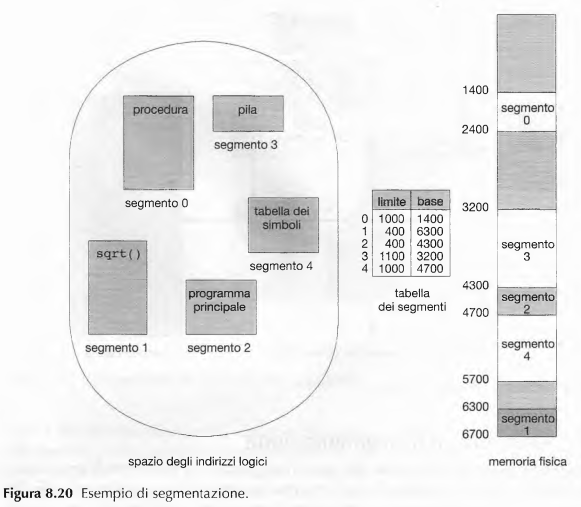
\includegraphics[scale=0.6]{img/0040.png}
\end{center}

\section{Memoria virtuale}
La \textbf{memoria virtuale} è una tecnica che permette di eseguire processi che possono an­che non essere completamente contenuti in memoria. Il vantaggio principale offerto da
questa tecnica è quello di permettere che i programmi siano più grandi della memoria fisica; inoltre la memoria virtuale astrae la memoria centrale in un vettore di memorizzazione
molto grande e uniforme, separando la memoria logica, com'è vista dalFutente, da quella fisica.

La
memoria virtuale permette inoltre ai processi di condividere facilmente file e spazi d'indirizzi, e fornisce un meccanismo efficiente per la creazione dei processi.

È però diffìcile da realizzare e, se usata scorrettamente, può ridurre di molto le prestazioni del
sistema.

\subsection{Introduzione}
Gli algoritmi di gestione della memoria delineati sono necessari perché, per
l'attivazione di un processo, le istruzioni da eseguire si devono trovare all'interno della me­moria fisica. Il primo metodo per far fronte a tale requisito consiste nel collocare l'intero
spazio d'indirizzi logici del processo relativo in memoria fisica.

La condizione che le istruzioni debbano essere nella memoria fisica sembra tanto ne­
cessaria quanto ragionevole, ma purtroppo riduce le dimensioni dei programmi a valori
strettamente correlati alle dimensioni della memoria fisica. In molti casi non è necessario avere in memoria l'intero programma, ad esempio:
\begin{itemize}
  \item Spesso i programmi dispongono di codice per la gestione di condizioni d'errore insoli­te. Poiché questi errori sono rari, se non inesistenti, anche i relativi segmenti di codice non si eseguono quasi mai.
  \item Spesso a array, liste e tabelle si assegna più memoria di quanta sia effettivamente ne­cessaria.
  \item Alcune opzioni e caratteristiche di un programma sono utilizzabili solo di rado.
\end{itemize}
La possibilità di eseguire un programma che si trova solo parzialmente in memoria
può essere vantaggiosa per i seguenti motivi:
\begin{itemize}
  \item Un programma non è più vincolato alla quantità di memoria fìsica disponibile. Gli utenti possono scrivere programmi per uno \textbf{spazio degli indirizzi virtuali}\index{spazio degli indirizzi virtuali} molto gran­de, semplificando così le operazioni di programmazione.
  \item Poiché ogni utente impiega meno memoria fisica, si possono eseguire molti più pro­grammi contemporaneamente, ottenendo un corrispondente aumento dell'utilizzo e della produttività della CPU senza aumentare il tempo di risposta o di completamento.
  \item Per caricare (o scaricare) ogni programma utente in memoria sono necessarie meno operazioni di I/O, quindi ogni programma utente è eseguito più rapidamente.
\end{itemize}

La \textbf{memoria virtuale} si fonda sulla separazione della memoria logica percepita dal­l'utente dalla memoria fisica.
L'espressione \textbf{spazio degli indirizzi virtuali} si riferisce alla collocazione dei processi in
memoria dal punto di vista logico (o virtuale).

È possibile organizzare la memoria fisica in frame di pagine; in questo caso i frame
delle pagine fisiche assegnati ai processi possono non essere contigui. Spetta all'unità di ge­stione della memoria (MMU) associare in memoria le pagine logiche alle pagine fisiche.

Si noti come allo heap sia lasciato sufficiente spazio per crescere ver­so l'alto nello spazio di memoria, poiché esso ospita la memoria allocata dinamicamente. In
modo analogo, consentiamo alla pila di svilupparsi verso il basso nella memoria, a causa di
ripetute chiamate di funzione. Lo spazio vuoto ben visibile (o buco) che separa lo heap dal­la pila è parte dello spazio degli indirizzi virtuali, ma richiede pagine fisiche realmente esi­stenti solo nel caso che lo heap o la pila crescano. Qualora contenga buchi, lo spazio degli
indirizzi virtuali si definisce sparso. Un simile spazio degli indirizzi consente di riempire i buchi grazie all'espansione dei segmenti heap o pila, e di collegare dinamicamente delle librerie (o altri oggetti condivisi) durante l'esecuzione del programma.
Oltre a separare la memoria logica da quella fìsica, la memoria virtuale offre, per due o
più processi, il vantaggio di condividere i file e la memoria, mediante la condivisione delle
pagine.
\begin{center}
  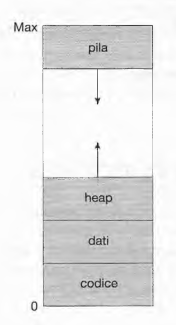
\includegraphics[scale=0.6]{img/0041.png}\\
  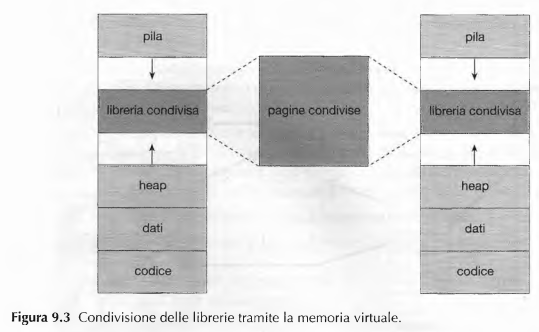
\includegraphics[scale=0.6]{img/0042.png}
\end{center}
Vantaggi:
\begin{itemize}
  \item Le librerie di sistema sono condivisibili da diversi processi associando l'oggetto condi­viso a uno spazio degli indirizzi virtuali, procedimento detto \textbf{mappatura}.
  \item Analogamente, la memoria virtuale rende i processi in grado di condividere la memoria. La memoria virtuale permette a un processo di creare una regione di memoria condivisibile da un altro processo. I processi che condividono questa regione la considerano parte del proprio spazio degli indirizzi virtuali, malgra­do le pagine fisiche siano, in realtà, condivise.
  \item La memoria virtuale può consentire, per mezzo della chiamata di sistema \texttt{fork()}, che le pagine siano condivise durante la creazione di un processo, così da velocizzare la ge­nerazione dei processi.
\end{itemize}

\subsection{Paginazione su richiesta}
Si consideri il caricamento in memoria di un eseguibile residente su disco. Una possibilità è
quella di caricare l'intero programma nella memoria fisica al momento dell'esecuzione.Però, all'inizio non è detto che serva avere tutto il programma in memoria.
Una strategia consiste nel caricare le pagine nel mo­mento in cui servono realmente (\textbf{paginazione su richiesta}). Secondo questo schema, le pagine sono caricate in memoria solo quando richieste durante l'esecuzione del programma: ne consegue che le pagine cui non si accede mai non sono mai caricate nella memoria fìsica.

Un sistema di paginazione su richiesta è analogo a un sistema paginato con avvicenda­mento dei processi in memoria. I processi risiedono in memoria se­condaria. Per eseguire un processo occorre cari­carlo in memoria. Tuttavia, anziché caricare in memoria l'intero processo, si può seguire un
criterio d'avvicendamento “pigro” (\emph{lazy swapping}):\index{swapping} non si carica mai in memoria una pagina
che non sia necessaria. Poiché stiamo considerando un processo come una sequenza di pagi­ne, invece che come un unico ampio spazio d'indirizzi contiguo, l'uso del termine \emph{avvicen­damento dei processi} non è appropriato. Nell'ambito della paginazione su richiesta, il modulo del sistema operativo che
si occupa della sostituzione delle pagine si chiama \textbf{paginatore}\index{paginatore} (\emph{pager}).

\subsubsection{Concetti fondamentali}
Quando un processo sta per essere caricato in memoria, il paginatore ipotizza quali pagine
saranno usate e trasferisce in memoria solo le pagine che ri­tiene necessarie.

Con tale schema è necessario che l'architettura disponga di un qualche meccanismo
che consenta di distinguere le pagine presenti in memoria da quelle nei dischi. A tal fine è
utilizzabile lo schema basato sul bit di validità. In questo caso,
però, il bit impostato come “valido” significa che la pagina corrispondente è valida ed è pre­sente in memoria; il bit impostato come “non valido” indica che la pagina non è valida (cioè non appartiene allo spazio d'indirizzi logici del processo) oppure è valida ma è attualmente
nel disco.

Se l'ipotesi del paginatore è esatta e si carica­no tutte e solo le pagine che servono effettivamente, il processo è eseguito proprio come se
fossero state caricate tutte le pagine. Durante l'esecuzione, il processo accede alle pagine re­sidenti in memoria, e l'esecuzione procede come di consueto.
Se il processo tenta l'accesso a una pagina che non era stata caricata in memoria, l'ac­cesso a una pagina contrassegnata come non valida causa un'\textbf{eccezione di pagina mancante}
\emph{(page fault trap}). L'architettura di paginazione, nota che il bit è non valido e invia un segnale di eccezione al sistema operati­vo; tale eccezione è dovuta a un “insuccesso” del sistema operativo nella scelta delle pagine da caricare in memoria.

Procedura di gestione dell'eccezione di pagina mancante:
\begin{itemize}
  \item Si controlla una tabella interna per questo processo; in genere tale tabella è conservata insieme al blocco di controllo di processo (PCB), allo scopo di stabilire se il riferimen­to fosse un accesso alla memoria valido o non valido.
  \item Se il riferimento non era valido, si termina il processo. Se era un riferimento valido, ma la pagina non era ancora stata portata in memoria, se ne effettua l'inserimento.
  \item Si individua un frame libero.
  \item Si programma un'operazione sui dischi per trasferire la pagina desiderata nel frame ap­pena assegnato.
  \item Quando la lettura dal disco è completata, si modificano la tabella interna, conservata con il processo, e la tabella delle pagine per indicare che la pagina si trova attualmente in memoria.
  \item Si riavvia l'istruzione interrotta dal segnale di eccezione. A questo punto il processo può accedere alla pagina come se questa fosse già presente in memoria.
\end{itemize}
È addirittura possibile avviare l'esecuzione di un processo senza pagine in memoria. Quan­do il sistema operativo carica nel contatore di programma l'indirizzo della prima istruzione
del processo, che è in una pagina non residente in memoria, il processo accusa un'assenza di
pagina. Una volta portata la pagina in memoria, il processo continua l'esecuzione, subendo
assenze di pagine fino a che tutte le pagine necessarie non si trovino effettivamente in me­moria. Lo schema de­scritto è una \textbf{paginazione su richiesta pura}.

I
meccanismi d'ausilio alla paginazione su richiesta che l'architettura del calcolatore
deve offrire sono quelli richiesti per la paginazione e l'avvicendamento dei processi in memoria:
\begin{itemize}
  \item \textbf{tabella delle pagine}: contrassegna un elemento come non valido attraverso un bit di validità oppure un valore speciale dei bit di protezione;
  \item \textbf{memoria secondaria}: conserva le pagine non presenti in memoria centrale. la sezione del disco usata a questo scopo si chia­ma \textbf{area d'avvicendamento}, o \textbf{area di scambio} (\emph{swap space}).
\end{itemize}
%
Uno dei requisiti cruciali della paginazione su richiesta è la possibilità di rieseguire una qua­lunque istruzione a seguito di un'eccezione di pagina mancante o assenza di pagina.

\subsubsection{Prestazioni della paginazione su richiesta}
La paginazione su richiesta può avere un effetto rilevante sulle prestazioni di un calcolatore.
Il motivo si può comprendere calcolando il tempo d'accesso effettivo per una memoria con
paginazione su richiesta. Attualmente, nella maggior parte dei calcolatori il tempo d'accesso
alla memoria, che si denota ma, varia da 10 a 200 nanosecondi. Finché non si verifichino as­senze di pagine, il tempo d'accesso effettivo è uguale al tempo d'accesso alla memoria. Se pe­rò si verifica un'assenza di pagina, occorre prima leggere dal disco la pagina interessata e
quindi accedere alla parola della memoria desiderata.
Supponendo che p sia la probabilità che si verifichi un'assenza di pagina ($0 < p < 1$), è
probabile che p sia molto vicina allo zero, cioè che ci siano solo poche assenze di pagine. Il
tempo d'accesso effettivo è dato dalla seguente espressione:\medskip\\
\emph{tempo d'accesso effettivo} $ = (1 - p) \times ma + p \times$ \emph{tempo di gestione dell'assenza di pagina}\medskip\\
Per calcolare il tempo d'accesso effettivo occorre conoscere il tempo necessario alla gestione
di un'assenza di pagina. Alla presenza di un'assenza di pagina si esegue la seguente sequenza:
\begin{itemize}
\item segnale d'eccezione al sistema operativo;
\item salvataggio dei registri utente e dello stato del processo;
\item controllo della correttezza del riferimento alla pagina e determinazione della locazione della pagina nel disco;
\item lettura dal disco e trasferimento in un frame libero:\\
- attesa nella coda relativa a questo dispositivo finché la richiesta di lettura non sia servita;\\
- attesa del tempo di posizionamento e latenza del dispositivo;\\
- inizio del trasferimento della pagina in un frame libero;
\item 6. durante l'attesa, allocazione della CPU a un altro processo utente (scheduling della
CPU, facoltativo);
\item ricezione di un'interruzione dal controllore del disco (I/O completato);
\item salvataggio dei registri e dello stato dell'altro processo utente (se è stato eseguito il pas­so 6);
\item verifica della provenienza dell'interruzione dal disco;
\item aggiornamento della tabella delle pagine e di altre tabelle per segnalare che la pagina ri­chiesta è attualmente presente in memoria;
\item attesa che la CPU sia nuovamente assegnata a questo processo;
\item recupero dei registri utente, dello stato del processo e della nuova tabella delle pagine, quindi ripresa dell'istruzione interrotta.
\end{itemize}
Non sempre sono necessari tutti i passi sopra elencati.
In ogni caso, il tempo di servizio dell'eccezione di pagina mancante comporta tre ope­
razioni principali:
\begin{itemize}
  \item servizio del segnale di eccezione di pagina mancante;
  \item lettura della pagina;
  \item riavvio del processo.
\end{itemize}
La prima e la terza operazione si possono realizzare, per mezzo di un'accurata codifica, in pa­recchie centinaia di istruzioni. Ciascuna di queste operazioni può richiedere da 1 a 100 mi­crosecondi. D'altra parte, il tempo di cambio di pagina è probabilmente vicino a 8 millise­condi. Un disco ha in genere un tempo di latenza di 3 millisecondi, un tempo di posiziona­mento di 5 millisecondi e un tempo di trasferimento di 0,05 millisecondi, quindi il tempo totale della paginazione è dell'ordine di 8 millisecondi, compresi i tempi d'esecuzione del codice relativo e delle operazioni dei dispositivi fisici coinvolti.
Il tempo effettivo d'acces­so in nanosecondi è il seguente:
\begin{center}
  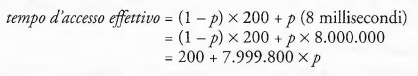
\includegraphics[scale=0.6]{img/0043.png}
\end{center}
Il tempo d'accesso effettivo è direttamente proporzionale alla \textbf{frequenza delle assenze di pa­gine} (\emph{page-fault rate}). Se un accesso su 1000 accusa un'assenza di pagina, il tempo d'accesso
effettivo è di 8,2 microsecondi. Impiegando la paginazione su richiesta, il calcolatore è ral­lentato di un fattore pari a 40. Se si desidera un rallentamento inferiore al 10\%, oc­corre che valgano le seguenti condizioni:
\begin{center}
  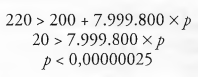
\includegraphics[scale=0.6]{img/0044.png}
\end{center}
Per mantenere a un livello ragionevole il rallentamento dovuto alla paginazione, si
può permettere meno di un'assenza di pagina ogni 399.990 accessi alla memoria.

Il file system funziona da memoria ausiliaria (\emph{backing store}). L'area d'avvicendamento si deve in ogni caso usare per le pagine che non sono re­lative ai file; queste comprendono la \textbf{pila} (\emph{stack}) e lo \textbf{heap} di un processo.

\subsection{Copiatura su scrittura}
Si è visto come un processo possa cominciare rapidamente l'esecuzione ri­chiedendo solo la pagina contenente la prima istruzione. La generazione dei processi trami­te \texttt{fork()}, però, può inizialmente evitare la paginazione su richiesta per mezzo di una tec­nica simile alla condivisione delle pagine, che garantisce la celere genera­zione dei processi riuscendo anche a minimizzare il numero di pagine allocate al nuovo processo.

Nella sua versione originale la \texttt{fork()} creava per il figlio una copia dello spa­zio d'indirizzi del genitore, duplicando le pagine appartenenti al processo genitore. Consi­derando che molti processi figli eseguono subito dopo la loro creazione la chiamata di siste­ma \texttt{exec()}, questa operazione di copiatura risulta inutile. In alternativa, si può impiegare
una tecnica nota come copiatura su scrittura (\emph{copy-on-write}) , il cui funzionamento si fonda
sulla condivisone iniziale delle pagine da parte dei processi genitori e dei processi figli. Le
pagine condivise si contrassegnano come pagine da copiare su scrittura, a significare che, se
un processo (genitore o figlio) scrive su una pagina condivisa, il sistema deve creare una copia di tale pagina.

Quando è necessaria la duplicazione di una pagina secondo la tecnica di copiatura su
scrittura, è importante capire da dove si attingerà la pagina libera necessaria. Molti sistemi
operativi forniscono, per queste richieste, un gruppo (\emph{pool}) di pagine libere, che di solito si
assegnano quando la pila o il cosiddetto heap di un processo devono espandersi. L'allocazione di queste pagine di solito avvie­ne secondo una tecnica nota come \emph{azzeramento su richiesta} (\emph{zero-fill-on-demand}); prima
dell'allocazione si riempiono di zeri le pagine, cancellandone in questo modo tutto il conte­nuto precedente.

Diverse versioni di UNIX offrono anche una variante della
chiamata di sistema \texttt{fork()} - detta \texttt{vfork()} (per \emph{virtual memory fork}). Con la \texttt{vfork()} il processo
genitore viene sospeso e il processo figlio usa lo spazio d'indirizzi del genitore. Poiché la
\texttt{vfork()} non usa la copiatura su scrittura, se il processo figlio modifica qualche pagina del­lo spazio d'indirizzi del genitore, le pagine modificate saranno visibili al processo genitore
non appena riprenderà il controllo. La
chiamata di sistema \texttt{vfork()} è adatta al caso in cui il processo figlio esegua una \texttt{exec()}
immediatamente dopo la sua creazione.

\subsection{Sostituzione delle pagine}
Nelle descrizioni fatte finora, la frequenza (\emph{rate}) delle assenze di pagine non è stata un pro­blema, giacché ogni pagina poteva essere assente al massimo una volta (la prima volta in cui si effettuava un riferimento a essa). Tale rappresentazione tuttavia non
è molto precisa. Se un processo di 10 pagine ne impiega effettivamente solo la metà, la pa­ginazione su richiesta fa risparmiare l'i/O necessario per caricare le cinque pagine che non
sono mai usate. Il grado di multiprogrammazione potrebbe essere aumentato eseguendo il
doppio dei processi. Quindi, disponendo di 40 frame, si potrebbero eseguire otto processi
anziché i quattro che si eseguirebbero se ciascuno di loro richiedesse 10 blocchi di memoria,
cinque dei quali non sarebbero mai usati.

Aumentando il grado di multiprogrammazione, si sovrassegna la memoria. Eseguen­do sei processi, ciascuno dei quali è formato da 10 pagine, di cui solo cinque sono effettiva­
mente usate, s'incrementerebbero l'utilizzo e la produttività della CPU e si risparmierebbero
10 frame. Tuttavia è possibile che ciascuno di questi processi, per un insieme particolare di
dati, abbia improvvisamente necessità di impiegare tutte le 10 pagine, perciò sarebbero ne­cessari 60 frame, mentre ne sono disponibili solo 40.


Si consideri inoltre che la memoria del sistema non si usa solo per contenere pagine di
programmi: le aree di memoria per l'I/O impegnano una rilevante quantità di memoria. Ciò
può aumentare le difficoltà agli algoritmi di allocazione della memoria. Al­cuni sistemi riservano una quota fissa di memoria per l'I/O, altri permettono sia ai processi
utenti sia al sottosistema di I/O di competere per tutta la memoria del sistema.

La \textbf{sovrallocazione}\index{sovrallocazione} (\emph{over-allocation}) si può illustrare come segue. Durante l'esecuzione
di un processo utente si verifica un'assenza di pagina. Il sistema operativo determina la loca­zione del disco in cui risiede la pagina desiderata, ma poi scopre che la lista dei frame liberi
è vuota: tutta la memoria è in uso.
A questo punto il sistema operativo può scegliere tra diverse possibilità, ad esempio
può terminare il processo utente. Tuttavia, gli utenti non devono sapere che i loro processi sono eseguiti su un sistema paginato. La pagi­nazione deve essere logicamente trasparente per l'utente, quindi la terminazione del proces­so non costituisce la scelta migliore.

Per realizzare la paginazione su richiesta è necessario risolvere due problemi principali:
occorre sviluppare un \textbf{algoritmo di allocazione dei frame} e un \textbf{algoritmo di sostituzione
delle pagine}.

Esistono molti algoritmi di sostituzione delle pagine; si sceglie quello con la mini­ma frequenza delle assenze di pagine (\emph{page-fault rate}).
Un algoritmo si valuta effettuandone l'esecuzione su una particolare \emph{successione di ri­ferimenti} alla memoria e calcolando il numero di assenze di pagine.

Di una pagina di date dimensioni, generalmente fissate dall'architettura
del sistema, si considera solo il numero della pagina anziché l'intero indirizzo. In secondo
luogo, quando si fa riferimento a una pagina \emph{p}, i riferimenti alla stessa pagina immediata­mente successivi al primo non accusano assenze di pagine: dopo il primo riferimento, la pa­gina \emph{p} è presente in memoria.\medskip\\
Facciamo un esempio:
\begin{center}
  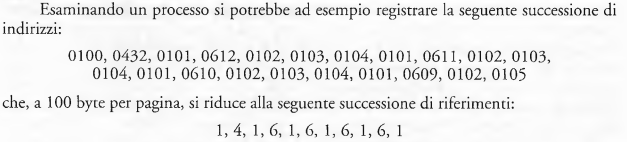
\includegraphics[scale=0.6]{img/0045.png}
\end{center}
Per stabilire il numero di assenze di pagine relativo a una particolare successione di riferi­menti e a un particolare algoritmo di sostituzione delle pagine, occorre conoscere anche il
numero dei frame disponibili. Naturalmente, aumentando il numero di quest'ultimi dimi­nuisce il numero di assenze di pagine. Per la successione dei riferimenti precedentemente
esaminata, ad esempio, dati tre o più blocchi di memoria si possono verificare tre sole assenze di pagine: una per il primo riferimento di ogni pagina. D 'altra parte, se si dispone di
un solo frame è necessaria una sostituzione per ogni riferimento, con il risultato di 11 as­senze di pagine. In generale è prevista una curva simile a quella della figura sotto. Aumen­tando il numero dei frame, il numero di assenze di pagine diminuisce fino al livello minimo.
Naturalmente aggiungendo memoria fisica il numero dei frame aumenta.
\begin{center}
  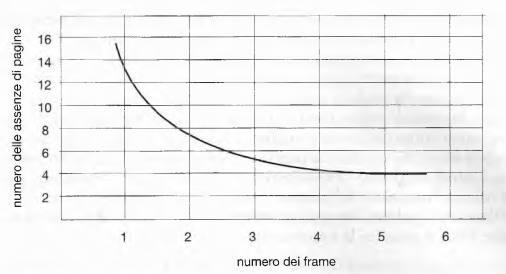
\includegraphics[scale=0.6]{img/0046.png}
\end{center}

\subsubsection{Sostituzione delle pagine secondo l'ordine di arrivo (FIFO)}
L'algoritmo di sostituzione delle pagine più semplice è un algoritmo FIFO. Se si
deve sostituire una pagina, si seleziona quella presente in memoria da più tempo. Non è strettamente necessario registrare l'istante in cui si carica una pagina in memoria; infatti si possono strutturare secondo una coda FIFO tutte le pagine presenti in me­moria. In questo caso si sostituisce la pagina che si trova nel primo elemento della coda.
Quando si carica una pagina in memoria, la si inserisce nell'ultimo elemento della coda\medskip\\
\begin{center}
  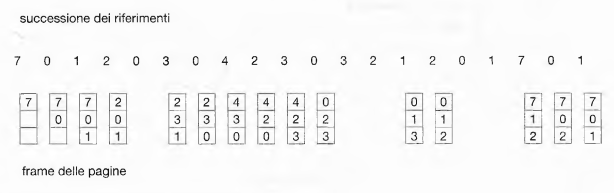
\includegraphics[scale=0.6]{img/0047.png}
\end{center}
Nella successione di riferimenti adottata, i nostri tre frame sono inizialmente vuoti. I
primi tre riferimenti (7, 0, 1) accusano ciascuno un'assenza di pagina con conseguente cari­camento delle relative pagine nei frame vuoti. Il riferimento successivo (2) causa la sostitu­zione della pagina 7, perché essa è stata caricata per prima in memoria. Siccome 0 è il riferi­mento successivo e si trova già in memoria, per questo riferimento non ha luogo alcuna as­senza di pagina. Il primo riferimento a 3 causa la sostituzione della pagina 0, che era la
prima fra le tre pagine in memoria (0, 1, e 2) da caricare. A causa di questa sostituzione il ri­ferimento successivo, a 0, accuserà un'assenza di pagina. La pagina 1 è allora sostituita dalla
pagina 0. Complessivamen­te si hanno 15 assenze di pagine.
\begin{center}
  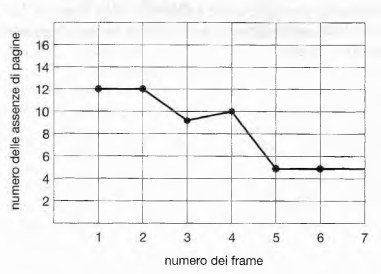
\includegraphics[scale=0.6]{img/0048.png}\\
  \caption{Curva delle assenze di pagine per sostituzione FIFO su una successione di riferimenti.}
\end{center}
L'algoritmo FIFO di sostituzione delle pagine è facile da capire e da programmare; tut­tavia la sue prestazioni non sono sempre buone.

Per illustrare i problemi che possono insorgere con l'uso deU'algoritmo di sostituzione
delle pagine FIFO, si consideri la seguente successione di riferimenti:
\begin{center}
1, 2, 3, 4, 1, 2, 5, 1, 2, 3, 4, 5
\end{center}
Il numero delle assenze di pagine (10) per quattro frame
è maggiore del numero delle assenze di pagine (9) per tre frame. Questo inatteso risultato è
noto col nome di \textbf{anomalia di Belady}.\index{Belady} Con alcuni algoritmi di sostitu­zione delle pagine, la frequenza delle assenze di pagine può aumentare con l'aumentare del
numero dei frame assegnati.

\subsubsection{Sostituzione ottimale delle pagine}
In seguito alla scoperta dell'anomalia di Belady, la ricerca si è diretta verso un algoritmo ot­timale di sostituzione delle pagine. Tale algoritmo è quello che fra tutti gli algoritmi pre­senta la minima frequenza di assenze di pagine e non presenta mai l'anomalia di Belady.
Questo algoritmo esiste ed è stato chiamato OPT o MIN.\index{algoritmo OPT o MIN} Semplicemente:
\emph{si sostituisce la pagina che non si userà per il periodo di tempo più lungo}.
\begin{center}
  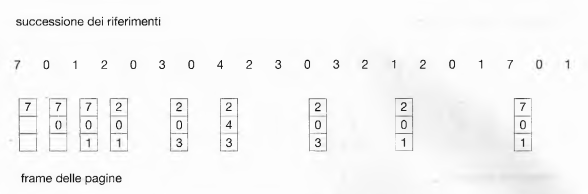
\includegraphics[scale=0.6]{img/0049.png}
\end{center}
Nella successione dei riferimenti considerata, l'algoritmo ottimale di sostituzio­ne delle pagine produce nove assenze di pagine.

Sfortunatamente l'algoritmo ottimale di sostituzione delle pagine è difficile da realiz­zare, perché richiede la conoscenza futura della successione dei riferimenti. Quindi, l'algoritmo ottimale si impiega soprattutto per studi comparativi.

\subsubsection{Sostituzione delle pagine usate meno recentemente (LRU)}
Se l'algoritmo ottimale non è realizzabile, è forse possibile realizzarne un'approssimazione: si sostituisce la
pagina che non è stata usata per il periodo più lungo. Il metodo appena descritto è noto co­me \textbf{algoritmo LRU}\index{algoritmo LRU} (\emph{least recently used}).
\begin{center}
  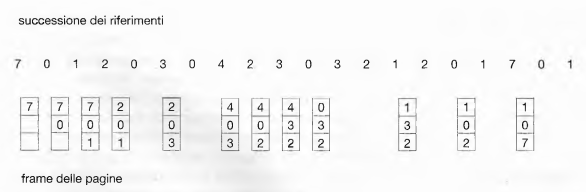
\includegraphics[scale=0.6]{img/0050.png}
\end{center}
L'algoritmo LRU produce 12 assenze di pagine.
\medskip\\
Il criterio LRU si usa spesso come algoritmo di sostituzione delle pagine ed è considera­to valido. Il problema principale riguarda la realizzazione della sostituzione stessa. Un algorit­mo di sostituzione delle pagine LRU può richiedere una notevole assistenza da parte dell'ar­chitettura del sistema di calcolo. Il problema consiste nel determinare un ordine per i frame
definito secondo il momento dell'ultimo uso. Si possono realizzare le due seguenti soluzioni:
\begin{itemize}
  \item \textbf{Contatori}. Nel caso più semplice, a ogni elemento della tabella delle pagine si associa un campo del momento d'uso, e alla CPU si aggiunge un contatore che si incrementa a ogni riferimento alla memoria. Questo schema implica una ricerca all'interno del­la tabella delle pagine per individuare la pagina usata meno recentemente (LRU), e una scrittura in memoria per ogni accesso alla memoria.
  \item Pila. Un altro metodo per la realizzazione della sostituzione delle pagine LRU prevede la presenza di una pila dei numeri delle pagine. Ogni volta che si fa un riferimento a una pagina, la si estrae dalla pila e la si colloca in cima a quest'ultima. In questo modo, in cima alla pila si trova sempre la pagina usata per ultima, mentre in fondo si trova la pagina usata meno recentemente. Poiché alcuni ele­menti si devono estrarre dal centro della pila, la migliore realizzazione si ottiene usan­do una lista doppiamente concatenata, con un puntatore all'elemento iniziale e uno a quello finale.
\end{itemize}
%
Né la sostituzione ottimale né quella LRU sono soggette all'anomalia di Belady; essi fanno parte di una classe di algoritmi di sostituzione delle pagine chiamati \textbf{algoritmi a pila}, che non presenta
l'anomalia di Belady.

\subsubsection{Sostituzione delle pagine per approssimazione a LRU}
Sono pochi i sistemi di calcolo che dispongono di un'architettura adatta a una vera sostitu­zione LRU delle pagine. Nei sistemi che non offrono tali caratteristiche specifiche si devono
impiegare altri algoritmi di sostituzione delle pagine, ad esempio l'algoritmo FIFO. Molti si­
stemi tuttavia possono fornire un aiuto: un bit di riferimento. Il bit di riferimento a una pagina è impostato automaticamente dall'architettura del sistema ogni volta che si fa un riferi­mento a quella pagina.

Inizialmente, il sistema operativo azzera tutti i bit. Quando s'inizia l'esecuzione di un
processo utente, l'architettura del sistema imposta a 1 il bit associato a ciascuna pagina cui si
fa riferimento. Dopo qualche tempo è possibile stabilire quali pagine sono state usate semplicemente esaminando i bit di riferimento. Non è però possibile conoscere l'ordine d'uso.

\subsubsection{Sostituzione delle pagine basata su conteggio}
\begin{itemize}
  \item \textbf{Algoritmo di sostituzione delle pagine meno frequentemente usate} (\emph{least frequently used}, LFU);\index{algoritmo LFU} richiede che si sostituisca la pagina con il conteggio più basso. Una pagina usata attivamente deve avere un conteggio di riferi­mento alto. Il punto debole di questo algoritmo è rappresentato dai casi in cui una pa­gina è usata molto intensamente durante la fase iniziale di un processo, ma poi non viene più usata. Poiché è stata usata intensamente il suo conteggio è alto, quindi rima­ne in memoria anche se non è più necessaria.
  \item \textbf{Algoritmo di sostituzione delle pagine più frequentemente usate} (\emph{most frequently used}, MFU)\index{algoritmo MFU}; è basato sul fatto che, probabilmente, la pagina con il contatore più basso è stata appena inserita e non è stata ancora usata.
\end{itemize}
Non sono molto comuni, poiché la realizzazione di questi algorit­mi è abbastanza onerosa; inoltre, tali algoritmi non approssimano bene la sostituzione OPT.

\subsubsection{Disco di basso livello}
Alcuni sistemi operativi permettono a certi programmi di
utilizzare una partizione del disco come un array sequenziale di blocchi logici, senza ricorre­re alle strutture di dati del file system. Un simile array è anche detto \textbf{disco di basso livello}
(\emph{raw disk}), e il relativo I/O è denominato \textbf{I/O di basso livello} (\emph{raw I/O}). Il disco di basso li­vello salta tutti i servizi del file system, come la paginazione su richiesta dei file in ingresso e in uscita, i lock dei file, il prefetching, l'allocazione dello spazio, i nomi dei file e le directo­ry. Sebbene alcune applicazioni siano più efficienti nel gestire i propri servizi specifici di memorizzazione sul disco di basso livello, quasi tutte hanno una resa migliore
quando operano con i servizi regolari del file system.

\subsection{Allocazione dei frame}
Occorre stabilire un criterio per l'allocazione della memoria libera ai diversi processi. é possibile considerare un caso in cui 93 frame liberi si debbano assegnare a due processi.

Il caso più semplice di memoria virtuale è il sistema con utente singolo. Si consideri un
sistema monoutente che disponga di 128 KB di memoria, con pagine di 1 KB. Complessiva­mente sono presenti 128 frame. Il sistema operativo può occupare 35 KB, lasciando 93 fra­me per il processo utente. In condizioni di paginazione su richiesta pura, tutti i 93 blocchi di memoria sono inizialmente posti nella lista dei frame liberi. Quando comincia l'esecuzio­ne, il processo utente genera una sequenza di eccezioni di pagine mancanti. Le prime 93 pa­gine assenti ricevono i frame liberi dalla lista. Una volta esaurita quest'ultima, per stabilire quale tra le 93 pagine presenti in memoria si debba sostituire con la novantaquattresima, si può usare un algoritmo di sostituzione delle pagine. Terminato il processo, si reinseriscono i 93 frame nella lista dei frame liberi.

Questa strategia è semplice, ma può subire molte variazioni. Si può richiedere che il si­stema operativo assegni tutto lo spazio richiesto dalle proprie strutture dati attingendo dalla lista dei frame liberi. Quando questo spazio è inutilizzato dal sistema operativo può essere sfruttato per la paginazione utente. Un'altra variante prevede di riservare sempre tre frame liberi, in modo che quando si verifica un'assenza di pagina sia disponibile un frame libero in cui trasferire la pagina richiesta. Mentre ha luogo il trasferimento della pagina, si può fare una sostituzione.

La strategia di base è chiara: al processo utente si assegna qualsiasi frame libero.

\subsubsection{Numero minimo di frame}
Le strategie di allocazione dei frame sono soggette a parecchi vincoli. Non si possono asse­gnare più frame di quanti siano disponibili, sempre che non vi sia condivisione di pagine. È necessario assegnare almeno un numero minimo di frame.
Una delle ragioni per allocare sempre un numero minimo di frame è legata alle presta­zioni. Ovviamente, al decrescere del numero dei frame allocati a ciascun processo aumenta la frequenza di mancanza di pagina, con conseguente ritardo dell'esecuzione dei processi.
Il numero minimo di frame è definito dall'hardware del calcolatore.

Il caso peggiore si può presentare nelle architetture di calcolatori che permettono rife­rimenti indiretti a più livelli (ad esempio quando ogni parola di 16 bit può contenere un in­dirizzo di 15 bit più un indicatore indiretto di 1 bit). In teoria, una semplice istruzione di caricamento può far riferimento a un indirizzo indiretto che a sua volta può far riferimento
a un indirizzo indiretto (su un'altra pagina) anch'esso facente riferimento a un indirizzo in­diretto su un'altra pagina ancora, e così via, finché tutte le pagine della memoria virtuale sia­no state chiamate in causa. Quindi, nel caso peggiore, tutta la memoria virtuale si deve tro­vare in memoria fisica. Per superare questa difficoltà occorre porre un limite al livello dei ri­ferimenti indiretti, ad esempio limitando un'istruzione a un massimo di 16 livelli. Quando
si verifica il riferimento indiretto di primo livello, si imposta un contatore al valore 16, per
decrementarlo a ciascun livello successivo relativo a questa istruzione. Se il contatore si ri­duce a 0 si verifica un segnale di eccezione.

Il numero minimo di frame per ciascun processo è definito dall'architettura, mentre il
numero massimo è definito dalla quantità di memoria fisica disponibile.

\subsubsection{Algoritmi di allocazione}
Il modo più semplice per suddividere m frame tra n processi è quello per cui a ciascuno si dà
una parte uguale, min frame. Dati 93 frame e cinque processi, ogni processo riceve 18 fra­me. I tre frame lasciati liberi si potrebbero usare come gruppo dei frame liberi. Questo schema è chiamato \textbf{allocazione uniforme}.

Un'alternativa consiste nel riconoscere che diversi processi hanno bisogno di quantità
di memoria diverse.

Per risolvere questo problema è possibile ricorrere all'\textbf{allocazione proporzionale}, se­condo cui la memoria disponibile si assegna a ciascun processo secondo la propria dimen­sione. Si supponga che $s_i$ sia la dimensione della memoria virtuale per il processo $p_i$. Si definisce la seguente quantità:
\[ S=\Sigma s_i \]
Quindi, se il numero totale dei frame disponibili è $m$, al processo $p_i$ si assegnano $a_i$ frame,
dove è approssimativamente
\[ a_i = \frac{s_i}{S \times m} \]
Naturalmente è necessario scegliere ciascun a{ in modo che sia un intero maggiore del nu­mero minimo di frame richiesti dalla struttura della serie di istruzioni di macchina e in mo­do che la somma di tutti gli $a_i$ non sia maggiore di $m$.


Sia nell'allocazione uniforme sia in quella proporzionale, l'allocazione a ogni processo
può variare rispetto al livello di multiprogrammazione. Se tale livello aumenta, ciascun processo perde alcuni frame per fornire la memoria necessaria per il nuovo processo. D'altra
parte, se il livello di multiprogrammazione diminuisce, i frame allocati al processo allonta­nato si possono distribuire tra quelli che restano.

Occorre notare che sia con l'allocazione uniforme sia con l'allocazione proporzionale,
un processo a priorità elevata è trattato come un processo a bassa priorità. Una soluzione prevede l'uso di uno schema di allocazione proporzionale in cui il rapporto dei frame non dipende dalle di­mensioni relative dei processi, ma dalle priorità degli stessi oppure da una combinazione di
dimensioni e priorità.

\subsubsection{Allocazione globale e allocazione locale}
Un altro importante fattore che riguarda il modo in cui si assegnano i frame ai vari processi
è la sostituzione delle pagine.
Gli algoritmi di sostituzione delle pagine si possono classificare in due categorie gene­rali: sostituzione globale e sostituzione locale. La sostituzione globale permette che per un
processo si scelga un frame per la sostituzione dall'insieme di tutti i frame, anche se quel
frame è correntemente allocato a un altro processo; un processo può dunque sottrarre un
frame a un altro processo. La sostituzione locale richiede invece che per ogni processo si scelga un frame solo dal proprio insieme di frame.

Si consideri uno schema di allocazione che, per una sostituzione a favore dei
processi ad alta priorità, permetta di sottrarre frame ai processi a bassa priorità. Per un pro­cesso si può stabilire una sostituzione che attinga tra i suoi frame oppure tra quelli di qualsia­si processo con priorità minore. Questo metodo permette a un processo ad alta priorità di au­mentare il proprio livello di allocazione dei frame a discapito del processo a bassa priorità.

Con la strategia di sostituzione locale, il numero di blocchi di memoria assegnati a un
processo non cambia. Con la sostituzione globale, invece, può accadere che per un certo pro­cesso si selezionino solo frame allocati ad altri processi, aumentando così il numero di frame
assegnati a quel processo, purché per altri non si scelgano per la sostituzione i \emph{propri} frame.
L'algoritmo di sostituzione globale risente di un problema: un processo non può con­trollare la propria frequenza di assenze di pagine (page-fault rate).

\subsubsection{Accesso non uniforme alla memoria}
I sistemi nei quali i tempi di accesso alla memoria variano in modo significativo sono gene­ralmente detti \textbf{sistemi con accesso non uniforme alla memoria} (\emph{non-uniform memory access},
NUMA) e sono più lenti dei sistemi nei quali memoria e processori risiedo­no sulla stessa scheda madre.

\subsection{Paginazione degenere (thrashing)}
Si consideri un qualsiasi processo che non disponga di un numero di frame “suf­ficiente”. Anche se tecnicamente si può ridurre al valore minimo il numero dei frame alloca­ti, esiste un certo numero di pagine in uso attivo. Se non dispone di que­sto numero di frame, il processo accusa immediatamente un'assenza di pagina. A questo pun­to si deve sostituire qualche pagina; ma, poiché tutte le sue pagine sono in uso attivo, si deve sostituire una pagina che sarà immediatamente necessaria, e di conseguenza si verificano su­bito parecchie assenze di pagine. Il processo continua a subire assenze di pagine, facendo so­stituire pagine che saranno immediatamente trattate come assenti e dovranno essere riprese.
Questa intensa quanto degenere paginazione (nota come \emph{thrashing})\index{thrashing} si verifica quando
si spende più tempo per la paginazione che per l'esecuzione dei processi.

\subsubsection{Cause della paginazione degenere}
La degenerazione dell'attività di paginazione causa parecchi problemi di prestazioni.

Si consideri il seguente scenrio: il sistema operativo vigila sull'utilizzo della CPU. Se questo è basso, aumenta il grado di
multiprogrammazione introducendo un nuovo processo. Si usa un algoritmo di sostituzione delle pagine globale, che sostituisce le pagine senza tener conto del processo al quale apparten­gono. Si ipotizzi che un processo entri in una nuova fase d'esecuzione e richieda più fra­me; se ciò si verifica si ha una serie di assenze di pagine, cui segue la sottrazione di nuove pagi­ne ad altri processi. Questi processi hanno però bisogno di quelle pagine e quindi subiscono
anchessi delle assenze di pagine, con conseguente sottrazione di pagine ad altri processi. Per ef­fettuare il caricamento e lo scaricamento delle pagine per questi processi si deve usare il dispo­sitivo di paginazione. Mentre si mettono i processi in coda per il dispositivo di paginazione, la
coda dei processi pronti per l'esecuzione si svuota, quindi l'utilizzo della CPU diminuisce.
Lo scheduler della CPU rileva questa riduzione dell'utilizzo della CPU e aumenta il gra­do di multiprogrammazione. Si tenta di avviare il nuovo processo sottraendo pagine ai pro­cessi in esecuzione, causando ulteriori assenze di pagine e allungando la coda per il disposi­tivo di paginazione. L'utilizzo della CPU scende ulteriormente, e lo scheduler della CPU ten­ta di aumentare ancora il grado di multiprogrammazione. L'attività di paginazione è
degenerata in una situazione patologica che fa precipitare la produttività del sistema. La fre­quenza delle assenze di pagine aumenta in modo impressionante, e di conseguenza aumen­ta il tempo effettivo d'accesso alla memoria. I processi non svolgono alcun lavoro, poiché si
sta spendendo tutto il tempo nell'attività di paginazione.

Aumentando il grado di multiprogrammazio­ne aumenta anche l'utilizzo della CPU, anche se più lentamente, fino a raggiungere un mas­simo. Se a questo punto si aumenta ulteriormente il grado di multiprogrammazione, l'atti­vità di paginazione degenera e fa crollare l'utilizzo della CPU. In questa situazione, per au­mentare l'utilizzo della CPU occorre ridurre il grado di multiprogrammazione.

Gli effetti di questa situazione si possono limitare usando un algoritmo di sostituzio­ne locale, o algoritmo di sostituzione per priorità. Con la sostituzione locale, se un proces­so ricade nell'attività di paginazione degenere, non può sottrarre frame a un altro processo e
quindi provocarne a sua volta la degenerazione. Le pagine si sostituiscono tenendo conto del
processo di cui fanno parte. Tuttavia, se i processi la cui attività di paginazione degenera ri­mangono nella coda d'attesa del dispositivo di paginazione per la maggior parte del tempo.
\begin{center}
  \includegraphics[scale=0.6]{img/0051.png}
\end{center}
Per evitare il verificarsi di queste situazioni, occorre fornire a un processo tutti i frame di cui
necessita. Per cercare di sapere quanti frame “servano” a un processo si impiegano diverse
tecniche.

\subsubsection{Modello dell'insieme del lavoro}
Il modello dell'insieme di lavoro (\emph{working-set model})working-set model usa un parametro, $\Delta$, per definire la \textbf{finestra dell'insieme di lavoro}. L'idea consiste nell'esaminare i più recenti $\Delta$ riferimenti alle pagine. L'insieme di pa­gine nei più recenti $\Delta$ riferimenti è l'\emph{insieme di lavoro}. Se una pagina è in uso attivo si trova nell'insieme di lavoro; se non è più usata esce dal­l'insieme di lavoro $\Delta$ unità di tempo dopo il suo ultimo riferimento. Quindi, l'insieme di la­voro non è altro che un'approssimazione della località\footnote{Una località è un insieme di pagine usate attivamente.} del programma.

La precisione dell'insieme di lavoro dipende dalla scelta del valore di $\Delta$. Se $\Delta$ è troppo
piccolo non include l'intera località, se è troppo grande può sovrapporre più località. Al li­mite, se $\Delta$ è infinito l'insieme di lavoro coincide con l'insieme di pagine cui il processo fa ri­ferimento durante la sua esecuzione.
La caratteristica più importante dell'insieme di lavoro è la sua dimensione. Calcolan­do la dimensione dell'insieme di lavoro, $WSS_i$ per ciascun processo $P_i$ del sistema, si può de­terminare la richiesta totale di frame, cioè $D$:
\[D= \Sigma WSS_i \]
Quindi, il processo i
necessita di $WSS_i$ frame. Se la richiesta totale è maggiore del numero totale di frame liberi
$(D > m)$, la paginazione degenera, poiché alcuni processi non dispongono di un numero suf­ficiente di frame.

Una volta scelto $D$, Il
sistema operativo controlla Finsieme di lavoro di ogni processo e gli assegna un numero di
frame sufficiente, rispetto alle dimensioni del suo insieme di lavoro. Se i frame ancora liberi
sono in numero sufficiente, si può iniziare un altro processo. Se la somma delle dimensioni
degli insiemi di lavoro aumenta, superando il numero totale dei frame disponibili, il sistema
operativo individua un processo da sospendere. Il processo sospeso può essere ripre­so successivamente.
Questa strategia impedisce la paginazione degenere, mantenendo il grado di multipro­grammazione più alto possibile, quindi ottimizza l'utilizzo della CPU.

\subsubsection{Frequenza delle assenze di pagine}
Il modello delFinsieme di lavoro riscuote un discreto successo, ma appare un modo alquanto goffo per con­
trollare la degenerazione della paginazione. La strategia basata sulla \textbf{frequenza delle assenze
di pagine} (\emph{page fault frequency},\index{pafe fault frequency} PFF\index{PFF}) è più diretta.

Il problema specifico è la prevenzione della paginazione degenere. Si deve controllare la frequenza delle assenze di pagine. Se la
frequenza delle assenze di pagine è eccessiva, significa che il processo necessita di più frame.
Analogamente, se la frequenza delle assenze di pagine è molto bassa, il processo potrebbe di­sporre di troppi frame. Si può fissare un limite inferiore e un limite superiore per la fre­quenza desiderata delle assenze di pagine. Se la frequenza
effettiva delle assenze di pagine per un processo oltrepassa il limite superiore, occorre alloca­re a quel processo un altro frame; se la frequenza scende sotto il limite inferiore, si sottrae un
frame a quel processo.

\subsection{File mappati in memoria}
Si consideri la lettura sequenziale di un file sul disco per mezzo delle consuete chiamate di
sistema: \texttt{open()}, \texttt{read()} e \texttt{write()}. Ciascun accesso al file richiede una chiamata di si­stema e un accesso al disco. In alternativa, possiamo avvalerci delle tecniche di memoria vir­tuale analizzate. Gra­zie a questa soluzione, nota come mappatura dei file in memoria, una parte dello spazio de­gli indirizzi virtuali può essere associata logicamente al file.

\subsubsection{Meccanismo di base}
La mappatura di un file in memoria si realizza associando un blocco del disco a una o più
pagine residenti in memoria. L'accesso iniziale al file avviene tramite una normale richiesta
di paginazione, che causa un errore di pagina mancante. Tuttavia, una porzione del file, che
è pari a una pagina, è caricata dal file system in una pagina fisica. Ogni successiva lettura e scrittura del fi­le è gestita come accesso ordinario alla memoria, semplificando così l'accesso al file e il suo utilizzo, in quanto si permette al sistema di manipolare i file attraverso la memoria anziché
appesantire il sistema stesso con le chiamate t\texttt{read()} e \texttt{write()}.

Alcuni sistemi operativi prevedono un'apposita chiamata di sistema per la mappatura
dei dati; le chiamate ordinarie sono riservate a tutte le altre operazioni di I/O. Altri sistemi
possono mappare un file in memoria, anche in assenza di un'esplicita richiesta in tal senso.

Per consentire la condivisione dei dati, più processi possono essere autorizzati a map­pare contemporaneamente un file in memoria. Quanto scritto da uno di questi processi mo­difica i dati nella memoria virtuale e risulta visibile a tutti gli altri processi che pure mappano il file.

\subsection{Allocazione di memoria del kernel}
Quando un processo eseguito in modalità utente necessita di memoria aggiuntiva, le pagine
sono allocate dalla lista dei frame disponibili che il kernel mantiene.

Il kernel, tuttavia, per allocare la propria memoria, attinge spesso a una riserva di me­moria libera differente dalla lista usata per soddisfare i processi ordinari in modalità utente.
Questo avviene principalmente per due motivi:
\begin{itemize}
  \item Il kernel richiede memoria per strutture dati dalle dimensioni variabili. Deve quindi fare un uso oculato della memoria, tentando di contenere al minimo gli sprechi dovuti alla frammentazione.
  \item Le pagine allocate ai processi in modalità utente non devono necessariamente essere contigue nella memoria fisica. Alcuni dispositivi, però, interagiscono direttamente con la memoria fisica; di conse­guenza, possono richiedere memoria che risieda in pagine fisicamente contigue.
\end{itemize}

\subsubsection{Sistema buddy}
Il “sistema buddy” (\emph{sistema gemellare}) utilizza un segmento di grandezza fissa per l'allocazio­ne della memoria, contenente pagine fisicamente contigue. La memoria è assegnata me­diante un cosiddetto \textbf{allocatore-potenza-di-2}, che alloca memoria in unità di dimensioni pari a potenze di 2.

Consideriamo un esempio semplice e ipotizziamo che la grandezza di un segmento di
memoria sia inizialmente di 256 KB e che il kernel richieda 21 KB di memoria. In primo
luogo il segmento è suddiviso in due \emph{buddy} (“gemelli”), che chiameremo $A_S$ e $A_D$, ciascuno
dei quali misura 128 KB. Uno di questi è ulteriormente dimezzato in 2 buddy da 64 KB, di­ciamo $B_S$ e $B_D$. Poiché la minima potenza di 2 che superi 21 KB è pari a 32 KB, occorre sud­dividere ancora $B_S$ o $B_D$, in due buddy la cui dimensione è 32 KB; chiamiamoli $C_S$ e
$C_D$. Uno di loro è il segmento scelto per soddisfare la richiesta di 21 KB.

Questo sistema offre il vantaggio di poter congiungere rapidamente buddy adiacenti
per formare segmenti più grandi tramite una tecnica nota come \textbf{fusione} (\emph{coalescing}).

L'ovvio inconveniente di questo sistema è che l'arrotondamento per eccesso a una potenza di 2 può facilmente generare frammentazione all'interno dei segmenti allocati.

\subsubsection{Allocazione a lastre}
Una seconda strategia per assegnare la memoria del kernel è detta \textbf{allocazione a lastre} (\emph{slab
allocation}). Una \textbf{lastra} è composta da una o più pagine fisicamente contigue. Una \textbf{cache}
consiste di una o più lastre. Vi è una sola cache per ciascuna categoria di struttura dati del
kernel: una cache dedicata alla struttura dati che rappresenta i descrittori dei processi, una
dedicata agli oggetti che rappresentano i file, un'altra per i semafori, e così via. Ogni cache è
popolata da \textbf{oggetti}, istanze della struttura dati del kernel rappresentata dalla cache.

L'algoritmo di allocazione delle lastre utilizza le cache per memorizzare oggetti del
kernel.

Al principio, tutti gli oggetti nella cache sono
contrassegnati come liberi. Quando una struttura dati del kernel ha bisogno di un oggetto,
per soddisfare la richiesta l'allocatore può selezionare dalla cache qualunque oggetto libero;
l'oggetto tratto dalla cache è quindi contrassegnato come \textbf{usato}.
In Linux una lastra può essere in uno dei seguenti stati:
\begin{itemize}
  \item Piena. Tutti gli oggetti della lastra sono contrassegnati come usati.
  \item Vuota. Tutti gli oggetti della lastra sono contrassegnati come liberi.
  \item Parzialmente occupata. La lastra contiene oggetti sia usati sia liberi.
\end{itemize}
%
L'allocatore delle lastre, per soddisfare una richiesta, tenta in primo luogo di estrarre un og­getto libero da una lastra parzialmente occupata; se non ne esistono, assegna un oggetto li­bero da una lastra vuota; in mancanza di lastre vuote disponibili, crea una nuova lastra da
pagine fisiche contigue e la alloca a una cache.m
L'allocatore delle lastre offre, essenzialmente, due vantaggi:
\begin{itemize}
  \item Annulla lo spreco di memoria derivante da frammentazione. Ogni struttura dati del kernel ha una cache associata; ciascuna delle cache è composta da un numero variabile di lastre, suddivise in spezzoni di grandezza pari a quella degli oggetti rappresentati. Pertanto, quando il kernel esi­ge memoria per un oggetto, l'allocatore delle lastre restituisce la quantità esatta di me­moria necessaria per rappresentare l'oggetto.
  \item Le richieste di memoria possono essere soddisfatte rapidamente.
\end{itemize}

\subsection{Altre considerazioni}
Le due scelte fondamentali nella progettazione dei sistemi di paginazione sono la definizio­ne dell'algoritmo di sostituzione e della politica di allocazione. Si devono però fare anche molte altre considerazioni.

\subsubsection{Prepaginazione}
Una caratteristica ovvia per un sistema di paginazione su richiesta pura consiste nell'alto nu­mero di assenze di pagine che si verificano all'avvio di un processo.

La \textbf{prepagina­zione}\index{prepaginazione} rappresenta un tentativo di prevenire un così alto livello di paginazione iniziale.
In alcuni casi la prepaginazione può essere vantaggiosa. La questione riguarda sempli­cemente il suo costo, che deve essere inferiore al costo per l'assistenza delle corrispondenti
mancanze di pagina. Può accadere che molte pagine trasferite in memoria dalla prepagina­zione non siano usate.

\subsubsection{Dimensione delle pagine}
È raro che chi progetta un sistema operativo per un calcolatore esistente possa scegliere le di­mensioni delle pagine.

Un fattore da considerare nella scelta delle dimensioni di una pagina è la dimensione
della tabella delle pagine.

\subsubsection{Portata della TLB}
Il tasso di successi (hit ratio) di una TLB\index{TLB} si rife­risce alla percentuale di traduzioni di indirizzi virtuali risolte dalla TLB anziché dalla tabella
delle pagine. Il tasso di successi è evidentemente proporzionale al numero di elementi della
TLB. Tuttavia, la memoria associativa che si usa per costruire le TLB è costosa e consuma
molta energia.

La portata della TLB (TLB reach), esprime la quantità di me­moria accessibile dalla TLB, ed è dato semplicemente dal numero di elementi moltiplicato per la dimensione delle pagine. La TLB
dovrebbe contenere l'insieme di lavoro di un processo.
Se si rad­doppia il numero di elementi della TLB, se ne raddoppia la portata.
Un altro metodo per aumentare la portata della TLB consiste nell'aumentare la dimen­sione delle pagine oppure nell'impiegare diverse dimensioni delle pagine.
L'uso di diverse dimensioni delle pagine richiede però che la gestione della TLB sia
svolta dal sistema operativo e non direttamente dall'architettura.
La gestione della TLB svolta dal sistema operativo e non
esclusivamente dall'architettura com porta una penalizzazione delle prestazioni. Tuttavia, i
vantaggi dovuti all'aum ento del tasso di successi e della portata della TLB superano gli svan­taggi che derivano dalla riduzione della rapidità di traduzione degli indirizzi.

\subsubsection{Vincoli di I/O}
Quando si usa la paginazione su richiesta, talvolta occorre permettere che alcune pagine si
possano vincolare alla memoria (\emph{locked in memory}). Una situazione di questo tipo si presen­ta quando l'I/O si esegue verso o dalla memoria utente (virtuale).

A ogni frame si associa un bit di vincolo (\emph{lock bit});\index{lock bit} se tale bit è attivato, la pagina contenuta
in tale frame non può essere selezionata per la sostituzione. Per
scrivere dati in un nastro occorre vincolare alla memoria le pagine contenenti tali dati, quin­di il sistema può continuare come di consueto. Le pagine vincolate non si possono sostitui­re. Completato l'I/O, si rimuove il vincolo.

L'uso dei bit di vincolo può essere pericoloso: se un bit non viene mai disatti­vato, ad esempio a causa di un baco del sistema operativo, il frame relativo alla pagina vin­colata diventa inutilizzabile. Su un sistema a singolo utente, l'abuso di tale meccanismo può
causare danni soltanto allo stesso utente.

\section{Interfaccia del file system}
Per la maggior parte degli utenti il file system è l'aspetto più visibile di un sistema operativo.
Fornisce il meccanismo per la registrazione e l'accesso in linea a dati e programmi ap­partenenti al sistema operativo e a tutti gli utenti del sistema di calcolo. Il file system consi­ste di due parti distinte: un insieme di file, ciascuno dei quali contenente dati correlati, e
una struttura della directory, che organizza tutti i file nel sistema e fornisce le informazioni
relative.

\subsection{Concetto di file}
I calcolatori possono memorizzare le informazioni su diversi supporti, come dischi, nastri ma­
gnetici e dischi ottici. Il sistema operativo astrae il \emph{file}\index{file} dalle caratteristiche
fisiche dei propri dispositivi di memoria per definire un'unità di memoria logica.

Un file è un insieme di informazioni, correlate e registrate in memoria secondaria, cui
è stato assegnato un nome. In genere un file è formato da una sequenza di bit, byte, righe o record il cui significato è definito dal creatore e dall'utente del file stesso.

Un file ha una \textbf{struttura} definita secondo il tipo: un
file di testo è formato da una sequenza di caratteri organizzati in righe, e probabilmente pa­gine; un file sorgente è formato da una sequenza di procedure e funzioni, ciascuna delle qua­li è a sua volta organizzata in dichiarazioni seguite da istruzioni eseguibili; un file oggetto è
formato da una sequenza di byte, organizzati in blocchi, comprensibile al modulo di collegamento del sistema; un file eseguibile consiste di una serie di sezioni di codice che il carica­tore può caricare in memoria ed eseguire.

\subsubsection{Attributi dei file}
Ogni file ha un nome che si usa come riferimento. Ha poi altri attributi che possono variare secondo il sistema operativo, ma che tipi­camente comprendono i seguenti:
\begin{itemize}
  \item Nome.
  \item Identificatore. Si tratta di un'etichetta unica, di solito un numero, che identifica il file all'interno del file system; è il nome impiegato dal sistema per il file.
  \item Tipo.
  \item Locazione.
  \item Dimensione.
  \item Protezione. Le informazioni di controllo degli accessi controllano chi può leggere, scrivere o far eseguire il file.
  \item Ora, data e identificazione dell'utente.
\end{itemize}
Le informazioni sui file sono conservate nella struttura della directory, che risiede a sua vol­ta in memoria secondaria.

\subsubsection{Operazioni sui file}
Un file è un \emph{tipo di dato astratto}. Per definire adeguatamente un file è necessario conside­rare le operazioni che si possono eseguire su di esso:
\begin{itemize}
  \item Creazione. Trovare lo spazio nel file system e crea­re un nuovo elemento nella directory in cui registrare il nome del file, la sua posizione nel file system ed eventualmente altre informazioni.
  \item Scrittura. Per scrivere in un file è indispensabile una chiamata di sistema che specifichi il nome del file e le informazioni che si vogliono scrivere.
  \item Lettura. er leggere da un file è necessaria una chiamata di sistema che spe­cifichi il nome del file e la posizione in memoria dove collocare il successivo blocco del file.
  \item Riposizionamento.
  \item Cancellazione.
  \item Troncamento. Si potrebbe voler cancellare il contenuto di un file, ma man­tenere i suoi attributi. Invece di forzare gli utenti a cancellare il file e quindi a ricrear­lo, questa funzione consente di mantenere immutati gli attributi (a esclusione della lunghezza del file) pur azzerando la lunghezza del file e rilasciando lo spazio occupato.
\end{itemize}
%
Il sistema operativo mantiene una piccola tabella contenente informa­zioni riguardanti tutti i file aperti (detta, per l'appunto, \textbf{tabella dei file aperti})\index{tabella dei file aperti}. Quando si
richiede un'operazione su un file, questo viene individuato tramite un indice in tale tabella,
in questo modo si evita qualsiasi ricerca. Quando il file non è più attivamente usato viene
chiuso dal processo, e il sistema operativo rimuove l'elemento a esso associato dalla tabella
dei file aperti.
A ciascun file aperto sono associate le diverse seguenti informazioni:
\begin{itemize}
  \item Puntatore al file.
  \item Contatore dei file aperti.
  \item Posizione nel disco del file.
  \item Diritti d'accesso.
\end{itemize}
%
Alcuni sistemi operativi offrono la possibilità di applicare \textbf{lock}\index{lock} a un file aperto per proteggerlo dall'accesso concorrente di altri pro­cessi.

\subsubsection{Tipi di file}
\begin{center}
  \includegraphics[scale=0.6]{img/0059.png}
\end{center}
Una tecnica comune per realizzare la gestione dei tipi di file consiste nell'includere il ti­po nel nome del file. Il nome è suddiviso in due parti, un nome e un'estensione, di solito sepa­rate da un punto.

\subsection{Metodi d'accesso}
\subsubsection{Accesso sequenziale}
Il più semplice metodo d'accesso è l'\textbf{accesso sequenziale}: le informazioni del file si elabora­no ordinatamente, un record dopo l'altro; questo metodo d'accesso è di gran lunga il più co­mune, ed è usato, ad esempio, dagli editor e dai compilatori.
\begin{center}
  \includegraphics[scale=0.6]{img/0060.png}
\end{center}

\subsubsection{Accesso diretto}
Un altro metodo è l'\textbf{accesso diretto} (o \textbf{accesso relativo}). Si fonda su un mo­dello di file che si rifa al disco: i dischi permettono, infatti, l'accesso diretto a ogni blocco di file. Il file si considera come una sequenza numerata di blocchi o record che si possono leg­gere o scrivere in modo arbitrario: si può ad esempio leggere il blocco 14, quindi il blocco 53 e poi scrivere il blocco 7. Non esistono limiti all'ordine di lettura o scrittura di un file ad accesso diretto.

I file ad accesso diretto sono molto utili quando è necessario accedere immediatamen­te a grandi quantità di informazioni.

\subsubsection{Altri metodi d'accesso}
Sulla base di un metodo d'accesso diretto se ne possono costruire altri, che implicano gene­ralmente la costruzione di un indice per il file. L'\textbf{indice} contiene puntatori ai vari blocchi;
per trovare un elemento del file occorre prima cercare nell'indice, e quindi usare il puntato­re per accedere direttamente al file e trovare l'elemento desiderato.
\begin{center}
  \includegraphics[scale=0.6]{img/0061.png}
\end{center}
Questa struttura per­mette di compiere ricerche in file molto lunghi limitando il numero di operazioni di I/O.

\subsection{Struttura della directory e del disco}
\subsubsection{Directory con struttura ad albero}
Permette agli utenti di creare pro­prie sottodirectory e di organizzare i file di conseguenza. L'albero ha una directory radice (\emph{root directory}), e ogni file del sistema ha un unico nome di percorso.
\begin{center}
  \includegraphics[scale=0.6]{img/0062.png}
\end{center}
Normalmente, ogni utente dispone di una directory corrente. La directory corrente
deve contenere la maggior parte dei file di interesse corrente per il processo. Quando si fa un
riferimento a un file, si esegue una ricerca nella directory corrente; se il file non si trova in
tale directory, Futente deve specificare un nome di percorso oppure cambiare la directory
corrente facendo diventare tale la directory contenente il file desiderato. Per cambiare direc­tory corrente si fa uso di una chiamata di sistema che preleva un nome di directory come pa­rametro e lo usa per ridefinire la directory corrente. Quindi, l'utente può cambiare la pro­pria directory corrente ogni volta che lo desidera.\medskip\\
I nomi di percorso possono essere di due tipi: \emph{nomi di percorso assoluti} e \emph{nomi di
percorso relativi}. Un nome di percorso assoluto comincia dalla radice dell'albero; un nome di percorso relativo definisce un percorso che parte dalla directory corrente.

\subsubsection{Directory con struttura a grafo aciclico}
La struttura ad albero non ammette la \emph{condivisione} di file o directory. Un \textbf{grafo acicli­co} \index{grafo aciclico} permette alle directory di avere sottodirectory e file condivisi. Lo \emph{stesso} fi­le o la \emph{stessa} sottodirectory possono essere in due directory diverse. Il fatto che un file sia condiviso, o che lo sia una directory, non significa che ci siano due copie del file; esiste un solo file effettivo.
\begin{center}
  \includegraphics[scale=0.6]{img/0063.png}
\end{center}
I file e le sottodirectory condivisi si possono realizzare in molti modi. Un metodo diffu­so prevede la creazione di un nuovo elemento di directory, chiamato collegamento. Un \textbf{collegamento} (\emph{link}) è un puntatore a un altro file o un'altra directory.

\subsection{Montaggio di un file system}
Così come si deve \emph{aprire} un file per poterlo usare, per essere reso accessibile ai processi di un
sistema, un file system deve essere \emph{montato}.

La procedura di montaggio è molto semplice: si fornisce al sistema operativo il nome
del dispositivo e la sua locazione (detta punto di montaggio) nella struttura di file e direc­tory alla quale agganciare il file system. Il passo successivo consiste nella verifica da parte del sistema operativo della validità del file system contenuto nel dispositivo. Infine, il sistema operativo annota nella sua struttura della directory che un certo file system è montato al punto di montaggio specificato.

\subsection{Condivisione di file}
\subsubsection{Utenti multipli}
Se un sistema operativo permette l'uso del sistema da parte di più utenti, diventano particolarmente rilevanti i problemi relativi alla condivisione dei file, alla loro identificazione tra­mite nomi e alla loro protezione.

Per realizzare i meccanismi di condivisione e protezione, il sistema deve memorizzare e
gestire più attributi di directory e file rispetto a un sistema che consente un singolo utente.

La maggior parte dei sistemi ha adottato i concetti di \emph{proprietario} (o utente) e \emph{gruppo}. Il proprietario è l'utente che può cambiare gli attributi di un file o directory, concedere l'accesso e che, in generale, ha il maggior control­lo sul file o directory.

Gli identificatori del gruppo e del proprietario di un certo file o directory (ID) sono
memorizzati insieme con gli altri attributi del file.

\subsection{Protezione}
\subsubsection{Tipi d'accesso}
La necessità di proteggere i file deriva direttamente dalla possibilità di accedervi. I sistemi
che non permettono l'accesso ai file di altri utenti non richiedono protezione; quindi si può
ottenere una completa protezione proibendo l'accesso o si può permettere un
accesso totalmente libero senza alcuna protezione. Ciò che serve in realtà è un accesso con­trollato.
Si possono controllare distinte operazioni:
\begin{itemize}
  \item Lettura.
  \item Scrittura.
  \item Esecuzione.
  \item Aggiunta. Scrittura di nuove informazioni in coda ai file.
  \item Cancellazione
  \item Elencazione. Elencazione del nome e degli attributi dei file.
\end{itemize}
Si possono controllare anche altre operazioni, come ridenominazione, copiatura o modifica
dei file. Tuttavia, in molti sistemi queste funzioni di livello superiore si possono realizzare
tramite un programma di sistema che compie alcune chiamate di sistema di livello inferiore,
quindi è sufficiente garantire la protezione a livello inferiore.

\subsubsection{Controllo degli accessi}
Lo schema più generale per realizzare gli accessi dipendenti dall'identità consiste
nell'associare una \textbf{lista di controllo degli accessi} (\emph{access-control list}, ACL) a ogni file e direc­tory; in tale lista sono specificati i nomi degli utenti e i relativi tipi d'accesso consentiti.

Questo sistema ha il vantaggio di permettere complessi metodi d'accesso. Il problema
maggiore delle liste di controllo degli accessi è la loro lunghezza: per permettere a tutti di
leggere un file, la lista deve contenere tutti gli utenti con accesso per la lettura. Per condensarne la lunghezza, molti sistemi raggruppano gli utenti di ogni file in tre
classi distinte:
\begin{itemize}
  \item Proprietario. È l'utente che ha creato il file.
  \item Gruppo. Insieme di utenti che condividono il file e richiedono tipi di accesso simili.
  \item Universo. Tutti gli altri.
\end{itemize}

\subsubsection{Semantica della coerenza}
La \textbf{semantica della coerenza} è un importante criterio per la valutazione di qualsiasi file
system che consenta la condivisione dei file. Si tratta di una caratterizzazione del sistema che
specifica la semantica delle operazioni in cui più utenti accedono contemporaneamente a un
file condiviso. In particolare, questa semantica deve specificare quando le modifiche ai dati
apportate da un utente possano essere osservate da altri utenti.\medskip\\
\textbf{Semantica dei file condivisi immutabili} - una volta che un file è stato dichia­rato condiviso dal suo creatore, non può essere modificato.

\section{Realizzazione del file system}
Il file system è l'aspetto più visibile di un sistema operativo. Fornisce il meccanismo per la registrazione e l'accesso in linea a dati e programmi ap­partenenti al sistema operativo e a tutti gli utenti del sistema di calcolo. Il file system consi­ste di due parti distinte: un insieme di file, ciascuno dei quali contenente dati correlati, e
una struttura della directory, che organizza tutti i file nel sistema e fornisce le informazioni
relative.

Il file system risiede perma­nentemente nella memoria secondaria, progettata per contenere in modo permanente grandi quantità di dati.

\subsection{Concetto di file}
I dischi costituiscono la maggior parte della memoria secondaria in cui si conserva il file sy­stem. Hanno due caratteristiche importanti:
\begin{itemize}
  \item si possono riscrivere localmente; si può leggere un blocco dal disco, modificarlo e quindi scriverlo nella stessa posizione;
  \item è possibile accedere direttamente a qualsiasi blocco di informazioni del disco, quindi risulta semplice accedere a qualsiasi file,
\end{itemize}
%
Anziché trasferire un byte alla volta, per migliorare l'efficienza dell'I/O, i trasferimenti
tra memoria centrale e dischi si eseguono per blocchi. Ciascun blocco è composto da uno o
più settori.

Per fornire un efficiente e conveniente accesso al disco, il sistema operativo fa uso di
uno o più file system che consentono di memorizzare, individuare e recuperare facilmente i
dati. Un file system presenta due problemi di progettazione piuttosto diversi. Il primo ri­guarda la definizione dell'aspetto del file system agli occhi dell'utente. Questo compito im­plica la definizione di un file e dei suoi attributi, delle operazioni permesse su un file e della
struttura delle directory per l'organizzazione dei file. Il secondo riguarda la creazione di al­goritmi e strutture dati che permettano di far corrispondere il file system logico ai dispositi­vi fisici di memoria secondaria.

Il file system è generalmente composto da molti livelli distinti.
Ogni livello si serve delle funzioni dei livelli inferiori per crearne di nuove impiegate dai livelli superiori.
\begin{center}
  \includegraphics[scale=0.6]{img/0052.png}
\end{center}
\begin{itemize}
  \item Il \textbf{controllo dell'I/O}, costituito dai driver dei dispositivi e dai gestori dei segnali d'interruzione, si occupa del trasferimento delle informazioni tra memoria cen­trale e memoria secondaria. Un driver di dispositivo si può concepire come un traduttore che riceva comandi ad alto livello e che emette specifiche istruzioni di basso livello per i dispositivi.
  \item Il \textbf{file system di base} deve inviare dei generici comandi all'appropriato driver di dispositivo per leggere e scrivere blocchi fisici nel disco. Ogni blocco fisico si identifica col suo indirizzo numerico nel disco, ad esempio unità 1, cilindro 73, superficie 2, settore 10. Questo strato gestisce inoltre buffer di memoria e le cache\footnote{Le cache servono a conservare metadati di file system usati frequentemente, in modo da migliorare le prestazioni.} che conservano vari blocchi dei fi­le system, delle directory e dei dati.
  \item Il \textbf{modulo di organizzazione dei file} è a conoscenza dei file e dei loro blocchi logici, così come dei blocchi fisici dei dischi. Conoscendo il tipo di allocazione dei file usato e la locazione dei file, può tradurre gli indirizzi dei blocchi logici negli indirizzi dei blocchi fisici.
  \item Il \textbf{file system logico} gestisce i metadati. Gestisce la strutrora della directory per fornire al modulo di organizzazione dei file le informazioni di cui necessita, dato un nome simbolico di file. Mantiene le strutture di file tramite i blocchi di controllo dei file (\emph{file control block}, FCB), contenenti informazioni sui file, come la proprietà, i permessi, e la posizione del contenuto. È responsabile anche della protezione e della sicurezza.
\end{itemize}
Nei file system stratificati la duplicazione di codice è ridotta al minimo. Il controllo dell'I/O e il codice di base del file system, possono essere comuni a numerosi file system, che poi gestiscono il file system logico e i moduli per 1'organizzazione dei file secon­do le proprie esigenze. Sfortunatamente, la stratificazione può comportare un maggior overhead del sistema operativo, che può generare un conseguente decadimento delle prestazioni.

Esistono svariati tipi di file system al giorno d'oggi, e non è raro che i sistemi operati­vi ne prevedano più d'uno. Ad esempio, sebbene Linux possa fun­zionare con più di quaranta file system diversi, quello standard è noto come \textbf{file system este­so}, le cui versioni maggiormente diffuse sono ext2 ed ext3. Esistono anche file system discribuiti, ossia tali che un file system del server è montato da uno o più client in una rete.

\subsection{Realizzazione del file system}
Per permettere ai processi di richiedere l'accesso al contenuto dei file, i sistemi operativi of­frono le chiamate di sistema \texttt{open()} e \texttt{close()}.

\subsubsection{Introduzione}
Per realizzare un file system si usano parecchie strutture dati, sia nei dischi sia in memoria.
Queste strutture variano secondo il sistema operativo e il file system, ma esistono dei prin­cìpi generali.

Nei dischi, il file system tiene informazioni su come eseguire l'avviamento di un sistema operativo memorizzato nei dischi stessi, il numero totale di blocchi, il numero e
la locazione dei blocchi liberi, la struttura delle directory e i singoli file.
Fra le strutture presenti nei dischi ci sono le seguenti:
\begin{itemize}
  \item Il \textbf{blocco di controllo dell'avviamento} (\emph{boot control block}), contenente le informazioni necessarie al sistema per l'avviamento di un sistema operativo da quel volume. Di solito è il prim o blocco di un volume. Nell'UFS, si chiama \textbf{blocco d'avviamento} (boot block); nell'NTFS, \textbf{setto­re d'avviamento della partizione} (\emph{partition boot sector}).
  \item I blocchi di controllo dei volumi (\emph{volume control block}); ciascuno di loro contiene i dettagli riguardanti il relativo volume (o partizione), come il numero e la dimensione dei blocchi nel disco, il contatore dei blocchi liberi e i relativi puntatori, il contatore dei blocchi di controllo dei file liberi e i relativi puntatori. Nell'UFS si chiama \textbf{superblocco}; nell'NTFS si chiama \textbf{tabella principale dei file} (\emph{master file table}, MFT).
  \item Le \textbf{strutture delle directory} (una per file system) usate per organizzare i file. Nel caso dell'UFS com prendono i nomi dei file e i numeri di \textbf{inode}\index{inode}\footnote{Nei sistemi Unix, un inode (o i-node, abbreviazione di index node) è una struttura dati sul file system che archivia e descrive attributi base su file, directory o qualsiasi altro oggetto.} associati. Nel caso dell'NTFS sono memorizzate nella tabella principale dei file (\emph{master file table}).
  \item I \textbf{blocchi di controllo di file} (FCB), contenenti molti dettagli dei file, compresi i per­messi d'accesso ai relativi file, i proprietari, le dimensioni e le locazioni dei blocchi di dati.
\end{itemize}
Le informazioni tenute in memoria servono sia per la gestione del file system sia per miglio­rare le prestazioni attraverso l'uso di cache. I dati si caricano al momento del montaggio e si
eliminano allo smontaggio. Le strutture che vi possono essere incluse sono di diverso tipo:
\begin{itemize}
  \item la tabella di m ontaggio interna alla memoria che contiene informazioni relative a ciascun volume montato;
  \item la struttura della directory;
  \item la tabella generale dei file aperti;
  \item la tabella dei file aperti per ciascun processo;
  \item i buffer.
\end{itemize}
Le applicazioni, per creare un nuovo file, eseguono una chiamata al file system logico, il
quale conosce il formato della struttura della directory. Esso crea e alloca un nuovo FCB. Il sistema carica quindi la directory appropriata in memoria, la aggiorna con il nome del nuovo file e con il
blocco di controllo associato, e la scrive nuovamente sul disco.
\begin{center}
  \includegraphics[scale=0.6]{img/0053.png}\\
  \caption{Tipico blocco di controllo dei file}
\end{center}
Alcuni sistemi operativi, compreso UNIX, trattano le directory esattamente come i file, di­stinguendole con un campo per il tipo che indica che si tratta di una directory. Altri, dispongono di chiamate di sistema distinte per i file e le directory e trattano le directory come entità separate dai file.

Una volta creato un file, per essere usato per operazioni di I/O deve essere aperto. La
chiamata di sistema \texttt{open()} passa un nome di file al file system. Per controllare se il file sia
già in uso da parte di qualche processo, la chiamata \texttt{open()} dapprima esamina la tabella dei
file aperti in tutto il sistema; in caso affermativo, aggiunge un elemento alla tabella dei file
aperti del processo (per ogni processo che stia usando il file) che punta alla tabella dei file
aperti in tutto il sistema. Una volta aperto il file, se ne ricerca il nome all'interno della directory.
Una volta trovato il file, si copia l'FCB nella tabella generale dei file aperti, che tiene anche traccia del numero di processi che in quel momento hanno il file aperto.

Successivamente, si crea un elemento nella tabella dei file aperti del processo con un
puntatore alla tabella generale e con alcuni altri campi. Il nome dato all'ele­mento della tabella è \textbf{descrittore di file} (\emph{file descriptor}) in UNIX, e \textbf{handle del file} in Windows. Finché un file non viene chiuso, tutte le operazioni si compiono sulla tabella dei
file aperti usando questo elemento. Quando un processo chiude il file, si cancella il relativo elemento nella tabella dei file
aperti del processo e si decrementa il contatore associato al file nella tabella generale.

\subsubsection{Partizioni e montaggio}
Un disco si può configurare in vari modi, secondo il sistema operativo che lo gestisce. Si può
suddividere in più partizioni, oppure un volume può comprendere più partizioni su molte­
plici dischi. Trattiamo il primo caso.

Ciascuna partizione è priva di struttura logica (\emph{raw partition})\index{raw partition} se non contiene alcun fi­le system. Se nessun file system è appropriato, si usa un \textbf{disco privo di struttura logica} (\emph{raw
disk})\index{raw disk}. Il sistema operativo UNIX impiega una partizione priva di struttura per l'area d'avvicendamento dei processi.

Le informazioni relative all'avviamento del sistema si possono registrare in un'apposi­ta partizione, che anche in questo caso ha un proprio formato, poiché nella fase d'avvia­mento il sistema non ha ancora caricato i driver di dispositivo del file system e quindi non
può interpretarne il formato. Questa partizione consistein una serie sequenziale di
blocchi, che si carica in memoria come un'immagine. L'immagine d'avviamento può conte­nere più informazioni di quelle che servono per un singolo sistema operativo; i PC, ad esem­pio, si possono configurare per l'installazione di più sistemi operativi (\emph{dual-booted}). In questo caso l'area d'avviamento può contenere un modulo, detto caricatore d'av­viamento (\emph{boot loader}), capace di interpretare diversi file system e diversi sistemi operativi. Una volta caricato, può avviare uno dei sistemi operativi disponibili nei dischi. Ciascun di­sco può avere più partizioni, ognuna contenente un diverso tipo di file system e un sistema operativo differente.

Nella fase di caricamento del sistema operativo, si esegue il montaggio della partizione
radice (\emph{root partition}), che contiene il kernel del sistema operativo e in alcuni casi altri file di sistema. Durante l'operazione di montaggio, il sistema verifica che il dispositivo contenga un file system vali­do. Infine, il siste­ma annota nella struttura della \textbf{tabella di montaggio}\index{tabella di montaggio} in memoria che un file system è stato montato insieme al tipo di file system.

\subsubsection{File system virtuali}
I sistemi operativi moderni devono gestire contemporaneamente tipi di file system diversi.

Un metodo ovvio ma non ottimale per realizzare più tipi di file system è scrivere pro­cedure di gestione di file e directory separate per ciascun tipo di file system.

Per isolare le funzioni di base delle chiamate di sistema dai dettagli di realizzazione si
adoperano apposite strutture dati. In questo modo la realizzazione del file system si articola
in tre strati principali:
\begin{center}
  \includegraphics[scale=0.55]{img/0054.png}
\end{center}
Il secondo strato si chiama strato del file system virtuale (\emph{virtual file system}\index{virtual file system}, VFS\index{VFS}) e
svolge due funzioni importanti:
\begin{itemize}
  \item Separa le operazioni generiche del file system dalla loro realizzazione definendo un'in­terfaccia VFS uniforme.
  \item Permette la rappresentazione univoca di un file su tutta la rete.
\end{itemize}

\subsection{Realizzazione delle directory}
La selezione degli algoritmi di allocazione e degli algoritmi di gestione delle directory ha un
grande effetto sull'efficienza, le prestazioni e l'affidabilità del file system.

\subsubsection{Lista lineare}
Il più semplice metodo di realizzazione di una directory è basato sull'uso di una lista lineare
contenente i nomi dei file con puntatori ai blocchi di dati. Questo metodo è di facile programmazione, ma la sua esecuzione è onerosa in termini di tempo. Per creare un nuovo file
occorre prima esaminare la directory per essere sicuri che non esista già un file con lo stesso
nome, quindi aggiungere un nuovo elemento alla fine della directory. Per cancellare un file
occorre cercare nella directory il file con quel nome, quindi rilasciare lo spazio che gli era as­segnato.

Esistono vari metodi per riutilizzare un elemento della directory: si può contrasse­gnare l'elemento come non usato oppure può essere aggiunto a una lista di elementi di directory liberi. Per ridurre il
tempo di cancellazione di un file si può usare anche una lista concatenata.

Il vero svantaggio dato da una lista lineare di elementi di directory è dato dalla ricerca
lineare di un file. na lista ordinata permette una ricerca binaria e riduce il tempo medio di ri­cerca, tuttavia il requisito dell'ordinamento può complicare la creazione e la cancellazione di
file. In questo caso, può essere d'aiuto una struttura dati più raffi­nata, come un B-albero. Un vantaggio della lista ordinata è che consente di produrre l'elen­co ordinato del contenuto della directory senza una fase d'ordinamento separata.

\subsubsection{Tabella hash}
Un'altra struttura dati che si usa per realizzare le directory è la tabella hash. L'inserimento e la cancellazione sono abba­stanza semplici, anche se occorre prendere provvedimenti per evitare collisioni. Le maggiori difficoltà legate a una tabella hash sono la sua dimensione, che in genere
è fissa, e la dipendenza della funzione hash da tale dimensione. Alternativamente, ciascun elemento della tabella hash, anziché un singolo valore, può
essere una lista concatenata; ciò consente di risolvere le collisioni aggiungendovi il nuovo ele­
mento. Le ricerche vengono alquanto rallentate, ma è comunque più veloce di una ricerca lineare.

\subsection{Metodi di allocazione}
\subsubsection{Allocazione contigua}
Per usare il metodo di allocazione contigua, ogni file deve occupare un insieme di blocchi
contigui del disco. Con questo ordinamento l'accesso al blocco $b+1$ dopo il blocco $b$ non richiede normal­mente alcuno spostamento della testina. Il numero dei posizionamenti (\emph{seek}) richiesti per accedere a file il cui spazio è allocato in modo contiguo è trascurabile, così com'è trascurabile il tempo di ricerca (\emph{seek time}).
\begin{center}
  \includegraphics[scale=0.6]{img/0055.png}
\end{center}
Lallocazione contigua presenta però alcuni problemi; una difficoltà riguarda l'indivi­duazione dello spazio per un nuovo file.
Il problema generale è quello di soddisfare una richiesta di di­mensione $n$ data una lista di buchi liberi. I più comuni criteri di scelta di un buco libero da un insieme di buchi disponibili sono il \emph{first-fit} e il \emph{best-fit}. Questi algoritmi soffrono della \textbf{frammentazione esterna}.

Una strategia per prevenire la perdita di una quantità significativa di spazio sul disco a
causa della frammentazione esterna consiste nel copiare un intero file system su un altro di­sco o nastro. Quindi si liberava completamente il primo disco creando un ampio spazio li­bero contiguo. La procedura provvedeva poi a copiare nuovamente i file nel disco, asse­gnando tale spazio contiguo. Questo schema compatta efficacemente tutto lo spazio libero in uno spazio contiguo, risolvendo il problema della frammentazione. Il costo di questa compattazione è rappresentato dal tempo necessario.

Un altro problema che riguarda l'allocazione contigua è la determinazione della quan­tità di spazio necessaria per un file. Esiste il problema di conoscere la dimensione del file da creare. Per ridurre al minimo gli inconvenienti, alcuni sistemi operativi fanno uso di uno
schema di allocazione contigua modificato: inizialmente si assegna una porzione di spazio
contiguo, e se questa non è abbastanza grande si aggiunge un'altra porzione di spazio,
un'\emph{estensione}.

\subsubsection{Allocazione concatenata}
L'\textbf{allocazione concatenata} risolve tutti i problemi dell'allocazione contigua. Ogni file è composto da una lista concatenata di blocchi del disco i quali possono essere sparsi in qualsiasi punto del disco stesso. La directory contiene un pun­tatore al primo e all'ultimo blocco del file.

Ogni blocco contiene un puntatore al blocco successivo.
Questi puntatori non sono disponibili all'utente.

Per creare un nuovo file si crea semplicemente un nuovo elemento nella directory. Ogni elemento della directory ha un puntatore al primo blocco del file. Questo puntatore s'inizializza a \texttt{nil} (file vuoto). Per leggere un file occorre semplicemente leggere i blocchi seguendo i puntatori da un blocco all'altro. Con l'al­locazione concatenata non esiste frammentazione esterna e per soddisfare una richiesta si può usare qualsiasi blocco libero della lista. Inoltre non è necessario dichiarare la dimensione di un file al momento della sua creazione. Un file può continuare a crescere finché sono di­
sponibili blocchi liberi.
\begin{center}
  \includegraphics[scale=0.6]{img/0056.png}
\end{center}
L'allocazione concatenata presenta comunque alcuni svantaggi. Può essere usata in modo efficiente solo per i file ad accesso sequenziale. Un altro svantaggio dell'allocazione concatenata riguarda lo spazio richiesto per i pun­tatori. Se un puntatore richiede 4 byte di un blocco di 512 byte, allora lo 0,78\% del disco è usato per i puntatori anziché per le informazioni: ogni file richiede un po' più spazio di quanto ne richiederebbe altrimenti.
La soluzione più comune a questo problema consiste nel riunire un certo numero di
blocchi contigui in \textbf{cluster} (gruppi di blocchi), e nell'allocare i cluster anziché i blocchi.

Un altro problema riguarda l'affidabilità. Poiché i file sono tenuti insieme da puntato­ri sparsi per tutto il disco, s'immagini che cosa accadrebbe se un puntatore andasse perduto
o danneggiato.Una soluzione a tale problema consiste nell'usare liste doppiamente concatenate oppure nel memorizzare il nome del file e il relativo numero di blocco in ogni blocco; questi
schemi però sono ancora più onerosi per ogni file.

Una variante importante del metodo di allocazione concatenata consiste nell'uso della \textbf{tabel­la di allocazione dei file}\index{tabella di allocazione dei file} (\emph{file allocation table}, FAT\index{FAT}). Essa ottimizza il tempo d'accesso diretto ma può causare un significativo numero di posizionamenti della testina.
\begin{center}
  \includegraphics[scale=0.6]{img/0057.png}
\end{center}

\subsubsection{Allocazione indicizzata}
In mancanza di una FAT, l'allocazione concatenata non è in grado di sostenere un efficiente
accesso diretto. L'\textbf{allocazione indicizzata} risolve questo problema, rag­gruppando tutti i puntatori in una sola locazione: il \textbf{blocco indice}. Ogni file ha il proprio blocco indice: si tratta di un array d'indirizzi di blocchi del di­sco.
\begin{center}
  \includegraphics[scale=0.6]{img/0058.png}
\end{center}
Ogni file deve avere un blocco indice. é auspicabile che questo sia quanto più piccolo è possibile;
ma se il blocco indice è troppo piccolo non può contenere un numero di puntatori suffi­ciente per un file di grandi dimensioni. È necessario un meccanismo di gestione:
\begin{itemize}
  \item \textbf{Schema concatenato}. Per permettere la presenza di lunghi file è possibile collegare tra loro parecchi blocchi indice.
  \item \textbf{Indice a più livelli}. Una variante della rappresentazione concatenata consiste nell'impiego di un blocco indice di primo livello che punta a un insieme di blocchi indice di secondo livello che, a loro volta, puntano ai blocchi dei file.
  \item \textbf{Schema combinato}. Adottato nell'UFS, consiste nel tenere i primi 15 puntatori del blocco indice nell'\emph{inode} del file. I primi 12 di que­sti 15 puntatori puntano a \textbf{blocchi diretti}, cioè contengono direttamente gli indirizzi di blocchi contenenti dati del file. Quindi, i dati per piccoli file (non più di 12 bloc­chi) non richiedono un blocco indice distinto. Se la dimensione dei blocchi è di 4 KB, è possibile accedere direttamente fino a 48 KB di dati. Gli altri tre puntatori puntano a blocchi indiretti. Il primo puntatore è l'indirizzo di un \textbf{blocco in­diretto singolo}; è un blocco indice che non contiene dati, ma indirizzi di blocchi che contengono dati. Quindi c'è un puntatore di \textbf{blocco indiretto doppio} che contiene l'indirizzo di un blocco che a sua volta contiene gli indirizzi di blocchi contenenti puntatori agli effettivi blocchi di dati. L'ultimo puntatore contiene l'indi­rizzo di un \textbf{blocco indiretto triplo}.
\end{itemize}

\subsubsection{Prestazioni}
Per qualsiasi tipo d'accesso, l'allocazione contigua richiede un solo accesso per ottene­re un blocco. Poiché è facile tenere l'indirizzo iniziale del file in memoria, si può calcolare
immediatamente l'indirizzo del disco dell'i-esimo blocco, oppure del blocco successivo, e
leggerlo direttamente.

Con l'allocazione concatenata si può tenere in memoria anche l'indirizzo del blocco succes­sivo e leggerlo direttamente. Questo metodo è valido per l'accesso sequenziale mentre, per quel che riguarda l'accesso diretto, un accesso all'i-esimo blocco può richiedere i letture del disco. (Quindi da non usare per un'applicazione che richiede accessi diretti.)

L'allocazione indicizzata è più complessa. Le pre­stazioni dell'allocazione indicizzata dipendono dalla struttura dell'indice, dalla dimensione del file e dalla posizione del blocco desiderato.

\subsection{Gestione dello spazio libero}
Poiché la quantità di spazio dei dischi è limitata, è necessario riutilizzare lo spazio lasciato
dai file cancellati per scrivere nuovi file. Per tener traccia dello spazio libero in un disco, il sistema conserva una lista dello spazio
libero; vi sono registrati tutti gli spazi liberi, cioè non allocati ad alcun file o directory.

\subsubsection{Vettore di bit}
Spesso la lista dello spazio libero si realizza come \textbf{una mappa di bit}, o \textbf{vettore di bit}. Ogni
blocco è rappresentato da un bit: se il blocco è libero, il bit è 1, se il blocco è assegnato il
bit è 0.

Si consideri, ad esempio, un disco dove i blocchi 2, 3, 4, 5, 8, 9, 10, 11, 12, 13, 17,
18, 25, 26 e 27 sono liberi e gli altri sono allocati. La mappa di bit dello spazio libero è la se­guente:
\begin{center}
  \includegraphics[scale=0.6]{img/0064.png}
\end{center}
I vantaggi principali che derivano da questo metodo sono la sua relativa semplicità ed effi­cienza nel trovare il primo blocco libero o n blocchi liberi consecutivi nel disco.

\subsubsection{Lista concatenata}
Un altro metodo di gestione degli spazi liberi consiste nel collegarli tutti, tenere un punta­
tore al primo di questi in una speciale locazione del disco e caricarlo in memoria. Questo
primo blocco contiene un puntatore al successivo blocco libero, e così via. Questo schema non è efficiente; per attraversare la lista è infatti necessario leggere
ogni blocco, con un notevole tempo di I/O. Fortunatamente la necessità di attraversare la li­sta dello spazio libero non è frequente.

\subsubsection{Conteggio}
Anziché tenere una lista di $n$ indirizzi liberi, è sufficiente tenere l'indirizzo del primo blocco libero e il numero $n$ di blocchi liberi contigui che seguono il primo blocco.

\subsubsection{Mappe di spazio}
l file system ZFS di Sun è stato progettato per contenere un gran numero di file, directory e
persino di file system. ZFS crea metalastre ( metaslab ) per dividere lo spazio
sul dispositivo in parti che abbiano una dimensione gestibile. Un dato volume potrebbe
contenere centinaia di metalastre. Ogni metalastra è associata a una mappa di spazio. ZFS
utilizza l'algoritmo di conteggio per memorizzare informazioni riguardanti i blocchi liberi.
La mappa di spazio è un registro di tutte le attivi­tà del blocco (allocazione e liberazione), in ordine cronologico, in formato di conteggio.

\subsection{Efficienza e prestazioni}
I dischi tendo­no di solito a essere il principale collo di bottiglia per le prestazioni di un sistema, essendo i più lenti tra i componenti più rilevanti di un calcolatore.

\subsubsection{Efficienza}
L'uso efficiente di un disco dipende fortemente dagli algoritmi usati per l'allocazione del di­sco e la gestione delle directory. Facciamo alcuni esempi.
\begin{itemize}
  \item L'allocazione preventiva degli \emph{inode} e la loro distribuzione nel vo­lume migliorano le prestazioni del file system.
  \item Per ridurre la frammentazione, il BSD UNIX varia la dimensione del cluster al crescere della dimensione del file. Cluster più grandi si usano dove possono essere riempiti, mentre cluster più piccoli si usano per file di piccole dimensioni e per l'ultimo cluster di un file.
\end{itemize}

\subsection{Ripristino}
Poiché i file e le directory sono mantenuti sia in memoria centrale sia nei dischi, è necessa­rio aver cura di assicurare che il verificarsi di un malfunzionamento nel sistema non com­porti la perdita di dati o la loro incoerenza.

Un crollo del sistema può causare incoerenze tra le strutture dati del file system su di­sco, come le strutture delle directory, i puntatori ai blocchi liberi e i puntatori agli FCB libe­ri.
Operazioni
comuni come la creazione di un file possono comportare molti cambiamenti strutturali al­
l'interno del file system di un disco.
Anche i bachi nell'implementazione del file system, i controllori del disco, e
persino le applicazioni utente possono indurre errori nel file system.

I file system hanno sva­riati metodi per affrontare queste circostanze, a seconda delle strutture dati e degli algoritmi
del file system.

\subsubsection{Verifica della coerenza}
Un file system deve prima scoprire i problemi e poi cor­reggerli. Per scoprire gli errori vengono esaminati tutti i metadati su ogni file system per ve­rificare la coerenza del sistema.
Questo procedimento richiederà diversi
minuti, o addirittura delle ore, e avverrà tutte le volte che il sistema si avvia. In alternativa,
un file system può registrare il suo stato all'interno dei metadati del file system. All'inizio di
ogni serie di modifiche dei metadati è impostato un bit di stato per indicare che i metadati
sono in stato di modifica. Se tutti gli aggiornamenti dei metadati si completano con succes­so, il file system può azzerare quel bit. Se tuttavia il bit dello stato rimane impostato, entra
in funzione un verificatore della coerenza.

Il \textbf{verificatore della coerenza} confronta i dati delle directory con quelli contenuti nei blocchi dei
dischi, tentando di correggere ogni incoerenza.
Ad esempio, se si adotta uno schema di al­locazione concatenata con un puntatore da ciascun blocco al successivo, si può ricostruire
l'intero file e ricreare il corrispondente elemento nella directory analizzando i blocchi di dati. Diversamente, la perdita di un elemento di una directory in un sistema ad allocazione in­dicizzata potrebbe essere disastrosa, poiché ogni blocco di dati non contiene alcuna infor­mazione sugli altri blocchi di dati.

\subsubsection{File system con registrazione delle modifiche}
Gli algoritmi per il ripristino vengono applicati con successo al problema della verifica
della coerenza, realizzando i \textbf{file system orientati alle transazioni e basati sulla registrazio­ne delle modifiche} (\emph{log-based transaction-oriented file system}), noti anche come \textbf{file system
annotati}\index{file system annotati} (\emph{journaling file system}).

L'approccio della verifica della coerenza permette alle strutture di esibire incoerenze successivamente corrette grazie al ripri­stino. Questa strategia comporta tuttavia alcuni problemi.
Per esempio, l'incoerenza potrebbe rivelarsi irreparabile; il verificatore della coerenza potrebbe non essere in grado di
ripristinare le strutture, con una conseguente perdita di file o addirittura di intere directory; il verificatore potrebbe richiedere l'intervento umano per risolvere i
conflitti.

La soluzione a questo problema consiste nell5applicare agli aggiornamenti dei metada­
ti relativi al file system metodi di ripristino basati sulla registrazione delle modifiche.

Fondamentalmente, tutte le modifiche dei metadati si annotano in modo sequenziale
in un file di registrazione, detto \emph{log}. Ogni insieme di operazioni che esegue uno specifico
compito si chiama \textbf{transazione}. Una volta che le modifiche sono riportate nel file di regi­strazione, le operazioni si considerano portate a termine con successo (\emph{committed}) e la chia­
mata di sistema può restituire il controllo al processo utente, permettendogli di proseguire
la sua esecuzione. Nel frattempo, si applicano alle effettive strutture del file system le opera­zioni scritte nel log, e man mano che si eseguono si aggiorna un puntatore che indica quali
azioni sono state completate e quali sono ancora incomplete. Quando un'intera transazione
è stata completata, se ne rimuovono le annotazioni dal log, che è in realtà un buffer circola­re. I \textbf{buffer circolari} scrivono fino alla fine dello spazio disponibile, e poi ricominciano dal­
l'inizio, sovrascrivendo i vecchi contenuti.

Se si verifica un crollo del sistema, nel log ci potranno essere zero o più transazioni, che possono essere completate. L'unico problema che si può presentare
è il caso in cui una transazione sia fallita (\emph{aborted}), cioè non sia stata dichiarata terminata
con successo prima del crollo del sistema. In questo caso, si devono annullare tutti i cam­biamenti che erano stati applicati al file system dalla transazione, di nuovo mantenendo la
coerenza del file system. Questo ripristino è tutto ciò che è necessario fare dopo un crollo
del sistema, eliminando tutti i problemi concernenti la verifica della coerenza.

\printindex

\end{document}
